\clearpage

\subsection{Transparent without Survivability}\label{heuristic_Transp_Survivability}
\begin{tcolorbox}	
\begin{tabular}{p{2.75cm} p{0.2cm} p{10.5cm}} 	
\textbf{Student Name}  	&:& Eduardo Fernandes    (20/10/2018 - )\\
	&:& Pedro Coelho    (01/03/2018 - )\\
\textbf{Goal}          &:& Implement the heuristic model for the transparent transport mode without survivability.
\end{tabular}
\end{tcolorbox}


\vspace{11pt}
In the transparent transport mode (single-hop approach), the signals travel through the network in the optical domain between lightpaths. One advantage of this transport mode is that these networks require optical switching. This enables the realization of ongoing optical connections throughout several links without OEO (optical-electrical-optical) conversions. However, there are performed some conversions in some intermediate nodes.

Transparent optical connections creates lightpaths which require the assignment of a wavelength that will be used to be exchanged by wavelength converters in order to optimize the network and minimize the total CAPEX.

After the creation of the matrices and the network topology, it is necessary to apply the routing and grooming algorithms created. In the end, a report algorithm will be applied to obtain the best CAPEX result for the network in question.

We also must take into account the following particularity of this mode of transport:
\begin{itemize}
  \item $N_{OXC,n}$ = 1, \quad $\forall$ n that process traffic
  \item $N_{EXC,n}$ = 1, \quad $\forall$ n that process traffic
\end{itemize}

The minimization of the network CAPEX is made through the equation \ref{Capex_heuristic} where in this case for the cost of nodes we have in consideration the electric cost \ref{Capex_Node_EXC_heuristic} and the optical cost \ref{Capex_Node_OXC_heuristic}.\\

In this case the value of $P_{exc,c,n}$ is obtained by equation \ref{EXC_pexc_transparent_heuristic} for short-reach and by the equation \ref{EXC_pexc2_transparent_heuristic} for long-reach and the value of $P_{oxc,n}$ is obtained by equation \ref{OXC_poxc_transparent_heuristic}.\\

The equation \ref{EXC_pexc_transparent_heuristic} refers to the number of short-reach ports of the electrical switch with bit-rate $c$ in node $n$, $P_{exc,c,n}$, i.e. the number of tributary ports with bit-rate $c$ in node $n$ which can be calculated as

\begin{equation}
P_{exc,c,n} = \sum_{d=1}^{N} D_{nd,c}
\label{EXC_pexc_transparent_heuristic}
\end{equation}

\noindent
where $D_{nd,c}$ are the client demands between nodes $n$ and $d$ with bit rate $c$.\\

\noindent
In this case there is the following particularity:

\begin{itemize}
  \item When $n$=$d$ the value of client demands is always zero, i.e, $D_{nn,c}=0$
\end{itemize}

As previously mentioned, the equation \ref{EXC_pexc2_transparent_heuristic} refers to the number of long-reach ports of the electrical switch with bit-rate -1 in node n, $P_{exc,-1,n}$, i.e. the number of add ports of node n which can be calculated as

\begin{equation}
P_{exc,-1,n} = \sum_{j=1}^{N} f_{nj}^{od}
\label{EXC_pexc2_transparent_heuristic}
\end{equation}

\noindent
where $f_{nj}^{od}$ is the number of optical channels between node $n$ and node $j$ for all demand pairs (od).

\vspace{11pt}
The equation \ref{OXC_poxc_transparent_heuristic} refers to the number of line ports and the number of adding ports of node $n$ which can be calculated as

\begin{equation}
P_{oxc,n} = \sum_{j=1}^{N} 2 f_{nj}^{od} + \sum_{j=1}^{N} \lambda_{nj}
\label{OXC_poxc_transparent_heuristic}
\end{equation}

\noindent
where $f_{nj}^{od}$ refers to the number of line ports for all demand pairs (od) and $\lambda_{nj}$ refers to the number of add ports.\\

\vspace{11pt}
To implement this heuristic approach there are used algorithms made in Java in a programming software called Eclipse and they are tested in an open-source network program called Net2Plan. In the Net2Plan guide section \ref{net2plan_guide} there is an explanation on how to use and test them in this network planner.

In the next pages it will be described all the steps performed to obtain the final results in the transparent transport mode without survivability. In the figure below \ref{fluxogram_transp_surv} it is shown a fluxogram with the description of this transport mode approach.

\begin{figure}[H]
\centering
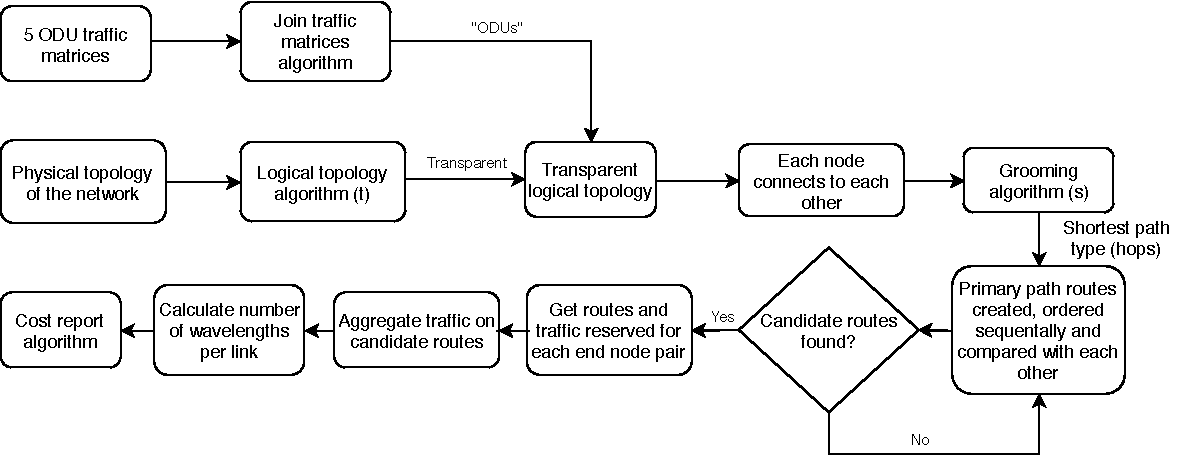
\includegraphics[width=16cm]{sdf/heuristic/transparent/figures/fluxogram_transparent_surv}
\caption{Fluxogram with the steps performed in the transparent without survivability transport mode approach.}
\label{fluxogram_transp_surv}
\end{figure}

\newpage
\subsubsection{Creation and join the traffic matrices}

\noindent
The first step is to create the traffic matrices based on the reference network \ref{Reference_Network_Topology}. In order to create the 5 traffic matrices in Net2Plan it is necessary the length of all the links and the total traffic used in this network, so later it is needed to define in Net2Plan the length in all end nodes and the total traffic depends on the value of traffic used (low traffic - 0.5 Tbit/s, medium traffic - 5 Tbit/s and high traffic - 10 Tbit/s). As you can see in the figure below, it is defined the path of the 5 ODUs and they will be aggregated in just one single ODU, making it possible to join all the demands in just one file and load it later into the network. This final resulting ODU joins the multiple traffic demands from all the traffic matrices previously created and, of course, the traffic demands will depend on the values used on the creation of the matrices (low, medium and high traffic).

\begin{figure}[H]
\centering
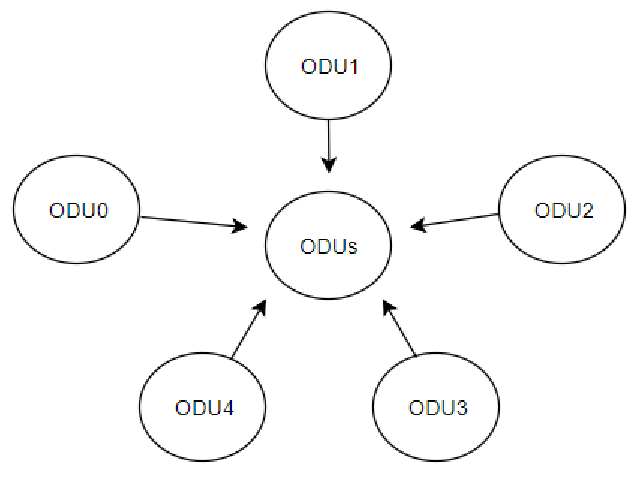
\includegraphics[width=7cm]{sdf/heuristic/transparent/figures/join_matrices_odus}
\caption{Join the 5 ODU traffic matrices into 1 single file "ODUs". The 5 traffic demands from the traffic matrices previously created are joined into 1 file to load it later on Net2Plan.}
\label{join_matrices_odus_transp_protec}
\end{figure}

\begin{figure}[H]
\centering
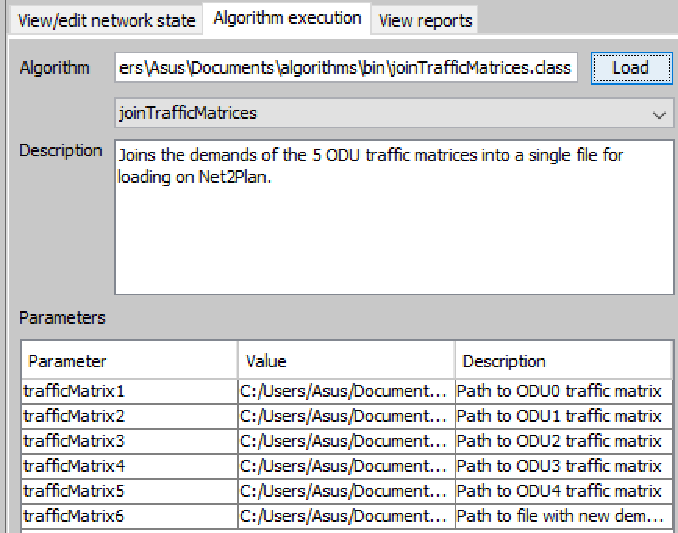
\includegraphics[width=8cm]{sdf/heuristic/transparent/figures/traffic_matrices}
\caption{Load of the join traffic matrices algorithm for the transparent transport mode on Net2Plan. It is defined the 5 paths to load the 5 ODU traffic matrices and the last path is the one where will be saved the file that joins all 5 the traffic demands.}
\label{traffic_matrices_transp_surv_ref}
\end{figure}

\newpage
\subsubsection{Creation of the physical topology}

\vspace{11pt}
The next step is to create the allowed physical topology of the network in Net2Plan. This network consists in 6 nodes and 8 bidirectional links. It is now also possible to define the length in all links. In the figure below it is shown the allowed physical topology in this transport mode.

\begin{figure}[H]
\centering
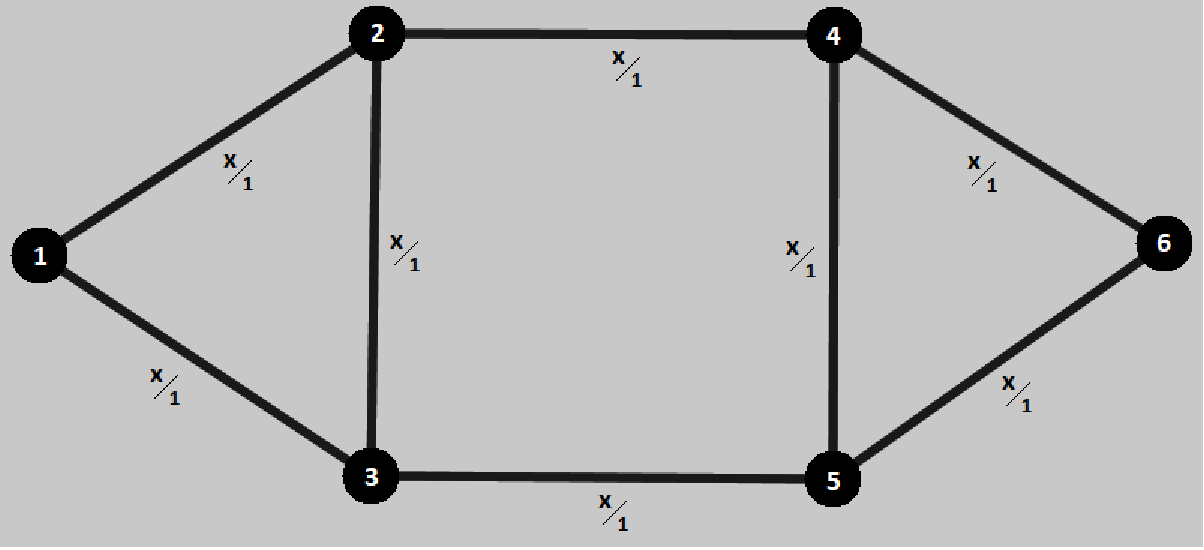
\includegraphics[width=12cm]{sdf/heuristic/transparent/figures/allowed_physical}
\caption{Allowed physical topology. The allowed physical topology is defined by the duct and sites in the field. It is assumed that each duct supports up to 1 bidirectional transmission system and each site supports up to 1 node.}
\label{allowed_physical_surv_transp}
\end{figure}

\subsubsection{Creation of the logical topology}

\vspace{11pt}
It is now time to create the allowed logical topology. A network topology represents how the links and the nodes of the network interconnect with each other and the logical topology algorithm creates the logical topology on another layer. In the transparent transport mode each node connects to each other creating direct links between all nodes in the network. Going through all nodes, if a node has a different index from other one, then creates a shortest and direct link between them. These additions of links between end nodes are made in the new upper layer of the network. The respective demands are saved in the new upper layer and those demands from the lower layer are then removed. The lower layer is the physical layer of the network and it is now created a new upper layer which is the logical layer of the network and represents the logical topology of the transparent transport mode.
The allowed physical and optical topologies, the logical topologies for all ODUs and the resulting physical topology is shown in the next section below \ref{result_description_transparent_heuristic_surv} for the three traffic scenarios. It is shown below three figures with the code in Java of the creation of the network logical topology, the load of the logical topology algorithm in Net2Plan and the resulting allowed optical topology for the transparent transport mode without survivability.

\begin{figure}[H]
\centering
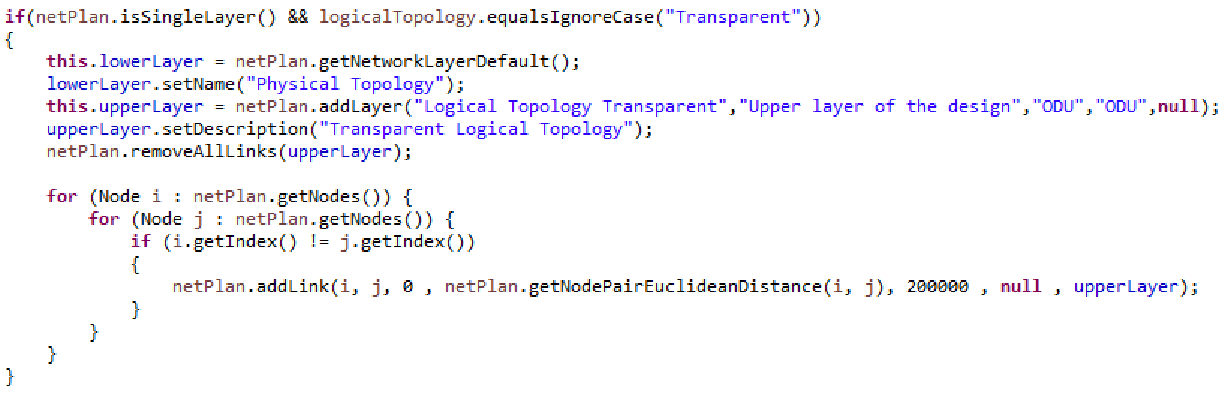
\includegraphics[width=15cm]{sdf/heuristic/transparent/figures/logical_topology_creation_transparent}
\caption{Java code of the logical topology approach for the transparent transport mode. The logical layer is created by adding direct links between all end nodes. The new layer is now the transparent logical topology of the network.}
\label{logical_topology_creation_transparent_surv}
\end{figure}

\begin{figure}[H]
\centering
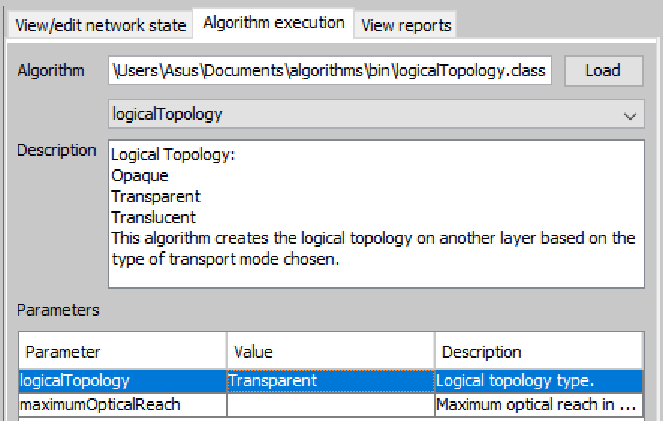
\includegraphics[width=10cm]{sdf/heuristic/transparent/figures/logical_topology_load_transparent}
\caption{Load of the logical topology algorithm for the transparent transport mode.}
\label{logical_topology_load_transparent_surv}
\end{figure}

\begin{figure}[H]
\centering
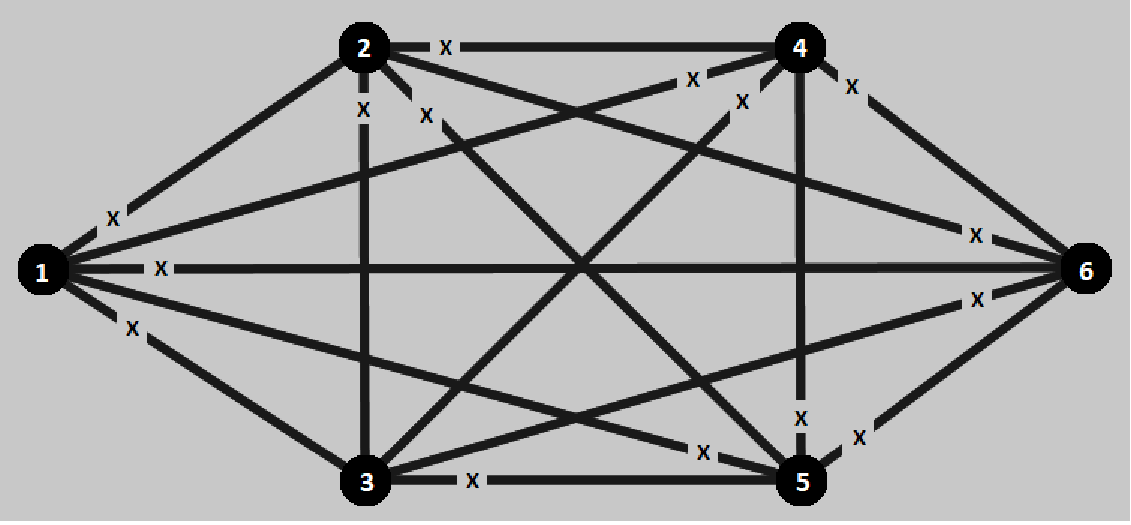
\includegraphics[width=10cm]{sdf/heuristic/transparent/figures/allowed_optical}
\caption{Allowed optical topology. It is assumed that each connections between demands supports up to 100 lightpaths.}
\label{allowed_optical_surv_transparent}
\end{figure}

\subsubsection{Creation of routes and aggregation of traffic}

\vspace{11pt}
After a network topology is created, it is now time to set the routing algorithm. In the transparent without survivability transport mode the routing algorithm is similar with the one used in opaque transport mode. It starts with going through all the demands and nodes which have different index between them (end nodes), create bidirectional routes (in this case the primary paths) based on the shortest path Dijkstra algorithm and then search the candidate routes for the respective demand. In this report it is used the shortest path type in hops. These routes are ordered sequentially and the shortest one per each demand is the primary path. The demands from the lower layer are removed and then saved in the upper layer. After this step, the routes are saved to a "Set" \ of routes and in each link of end nodes it is set the traffic demands into these routes that will integrate the whole network.

\begin{figure}[H]
\centering
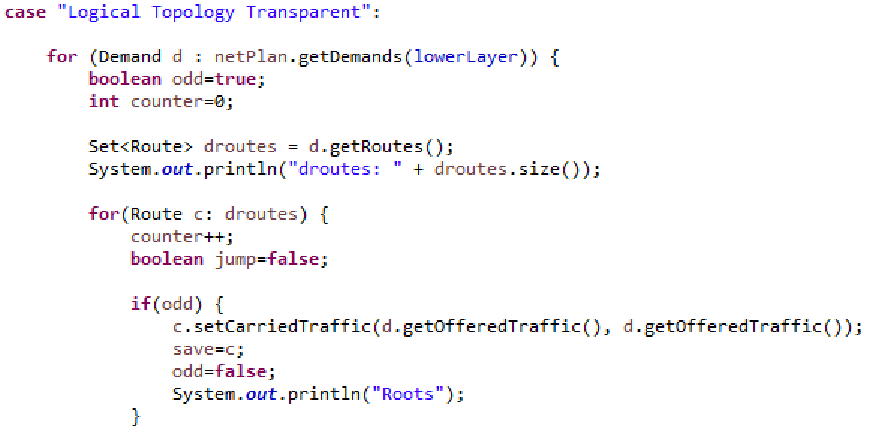
\includegraphics[width=14cm]{sdf/heuristic/transparent/figures/grooming_transparent_surv1}
\caption{Creation of routes and aggregation of traffic for the transparent without survivability transport mode. The candidate routes are searched by the shortest path type method and the offered traffic demands are set into these routes.}
\label{grooming_transparent_surv1}
\end{figure}

\begin{figure}[H]
\centering
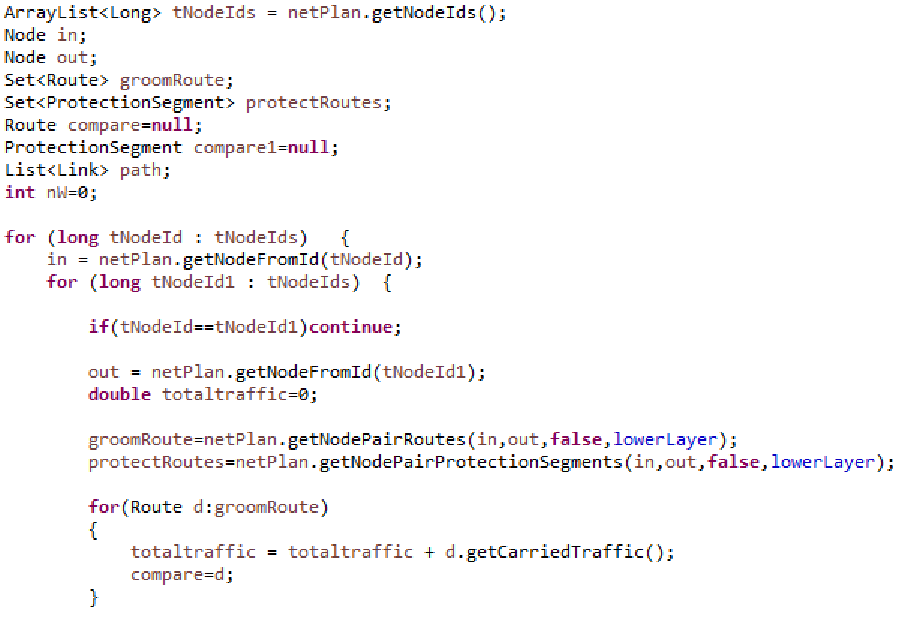
\includegraphics[width=14cm]{sdf/heuristic/transparent/figures/grooming_transparent_surv2}
\caption{Creation of routes and aggregation of traffic for the transparent without survivability transport mode. The traffic demands are set into the candidate primary path routes found earlier.}
\label{grooming_transparent_surv2}
\end{figure}

\begin{table}[H]
\centering
\begin{tabular}{|| c | c ||}
 \hline
 Function & Definition \\
 \hline\hline
 netPlan.getDemands(lowerLayer) & Returns the array of demands for the lower layer. \\
 \hline
 d.getRoutes() & Returns all the routes associated to the demand "d". \\
 \hline
 c.setCarriedTraffic() & \makecell{Sets the route carried traffic and the occupied capacity\\in the links, setting it up to be the same in all links.} \\
 \hline
 d.getOfferedTraffic() & Returns the offered traffic of the demand "d". \\
 \hline
 netPlan.getNodeIds() & Returns the array of the nodes' indexes. \\
 \hline
 netPlan.getNodeFromId(tNodeId) & Returns the node with the index "tNodeId". \\
 \hline
 \makecell{netPlan.getNodePairRoutes\\(in,out,false,lowerLayer)} &  \makecell{Returns the routes at "lowerLayer" \ \\from nodes "in" \ and "out".} \\
 \hline
\end{tabular}
\caption{Table with the description of the main functions in the creation of routes and aggregation of traffic in the grooming algorithm.}
\label{grooming_table_variables_transparent_surv}
\end{table}

\newpage
\subsubsection{Calculation of the number of wavelengths per link}

\vspace{11pt}
The final step of the routing and grooming algorithms is to calculate the number of wavelengths per link for the whole network. This is the last and an important step because with the number of wavelengths per link in the network, it is possible to calculate other network components. In the transparent transport mode, as in the figure below shows, the algorithm starts with going through all the nodes which have different index between them (end nodes) and in all the links that crosses between these pairs of nodes is reserved a link capacity based on the previous traffic aggregation. The total carried traffic in the link including protection and non-protection segments will be divided by the wavelength capacity and it is now possible to obtain the number of wavelengths per link.

\begin{figure}[H]
\centering
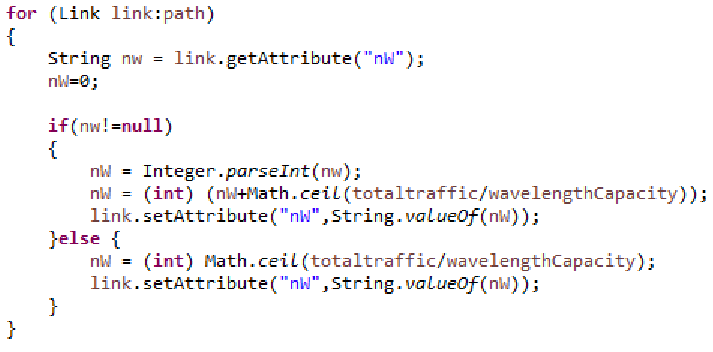
\includegraphics[width=13cm]{sdf/heuristic/transparent/figures/grooming_transparent_surv3}
\caption{Calculation of the number of wavelengths per link for the transparent transport mode. The link capacity is reserved based on the previous traffic aggregation.}
\label{grooming_transparent_surv3}
\end{figure}

\begin{figure}[H]
\centering
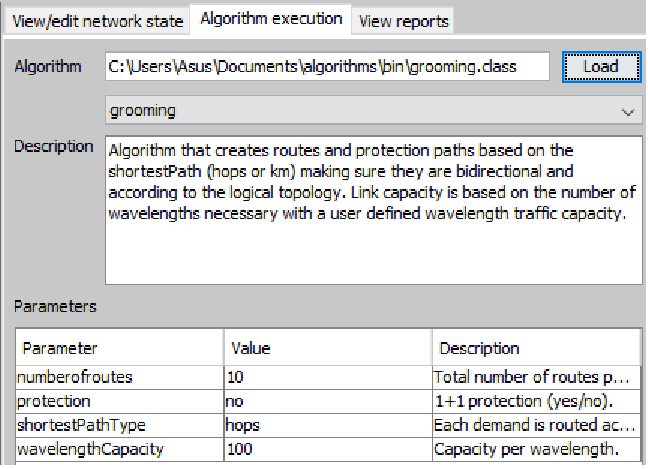
\includegraphics[width=11cm]{sdf/heuristic/transparent/figures/grooming_transparent_surv4}
\caption{Load of the grooming algorithm for the transparent without survivability transport mode. The total number of routes per demand is set to 10, the user can define if the model is with or without protection, the shortest path type is set to "hops" \ and the capacity per wavelength is used 100 optical channels.}
\label{grooming_transparent_surv4}
\end{figure}

\newpage
\subsubsection{Network cost report}

\vspace{11pt}
In order to obtain the network CAPEX results, the formulas needed to calculate the network elements and that are demonstrated previously in the beginning of this section \ref{heuristic_Transp_Survivability} were "translated" \ into Java code in a cost report algorithm. This algorithm can be loaded in Net2Plan and calculates and shows in tables the network CAPEX and also the per-link and per-node information with more details.

\begin{figure}[H]
\centering
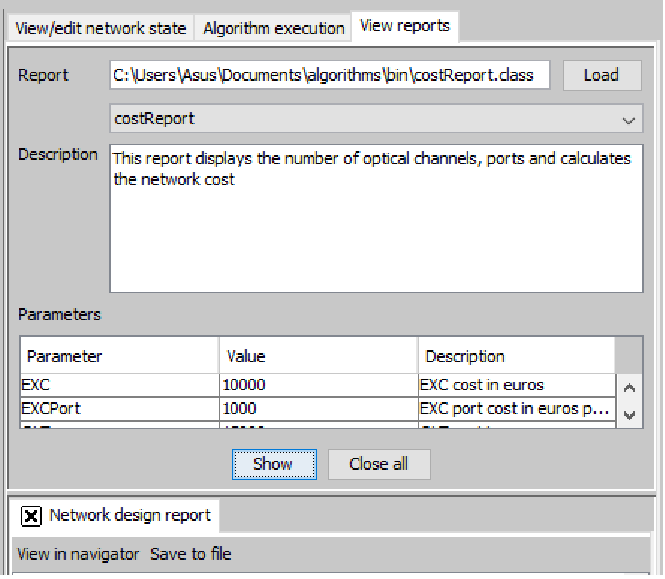
\includegraphics[width=10cm]{sdf/heuristic/transparent/figures/cost_report_transparent}
\caption{Load of the cost report algorithm on Net2Plan. The result view is an HTML page with the network optical and electrical components and their costs.}
\label{cost_report_transparent_surv}
\end{figure}

\newpage
\subsubsection{Result description}\label{result_description_transparent_heuristic_surv}

It is already known all the necessary formulas to obtain the CAPEX value for the reference network \ref{Reference_Network_Topology}. As described in the subsection of the network traffic \ref{Reference_Network_Traffic}, it is necessary to obtain three different values of CAPEX for the low (0.5 Tbit/s), medium (5 Tbit/s) and high (10 Tbit/s) traffic. It is used a network software program called Net2Plan which can design the traffic matrices, create all the network topologies, simulate the algorithms into the network implemented in the programming software called Eclipse and analyze the results obtained.\\
In this chapter will be demonstrated the results by Vasco's heuristics from 2016. In each of the three traffic scenarios, it will be shown the network topologies followed by the table with the CAPEX value of the network.\\

\noindent
\textbf{Low Traffic Scenario:}\\

In this scenario we have to take into account the traffic calculated in \ref{low_scenario}. In a first phase we will show the various existing topologies of the network. The first are the allowed topologies, physical and optical topologies, the second are the logical topology for all ODUs and finally the resulting physical topology.\\

\begin{figure}[H]
\centering
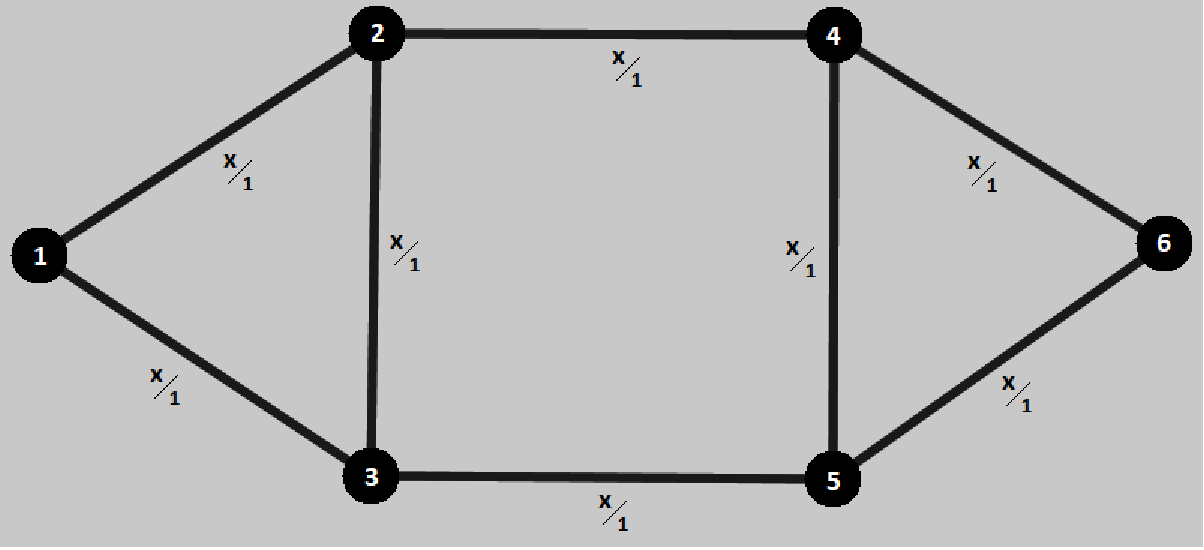
\includegraphics[width=13cm]{sdf/heuristic/transparent/figures/allowed_physical}
\caption{Allowed physical topology. The allowed physical topology is defined by the duct and sites in the field. It is assumed that each duct supports up to 1 bidirectional transmission system and each site supports up to 1 node.}
\label{allowed_physical_surv_ref_low_heuristic_transparent}
\end{figure}

\begin{figure}[H]
\centering
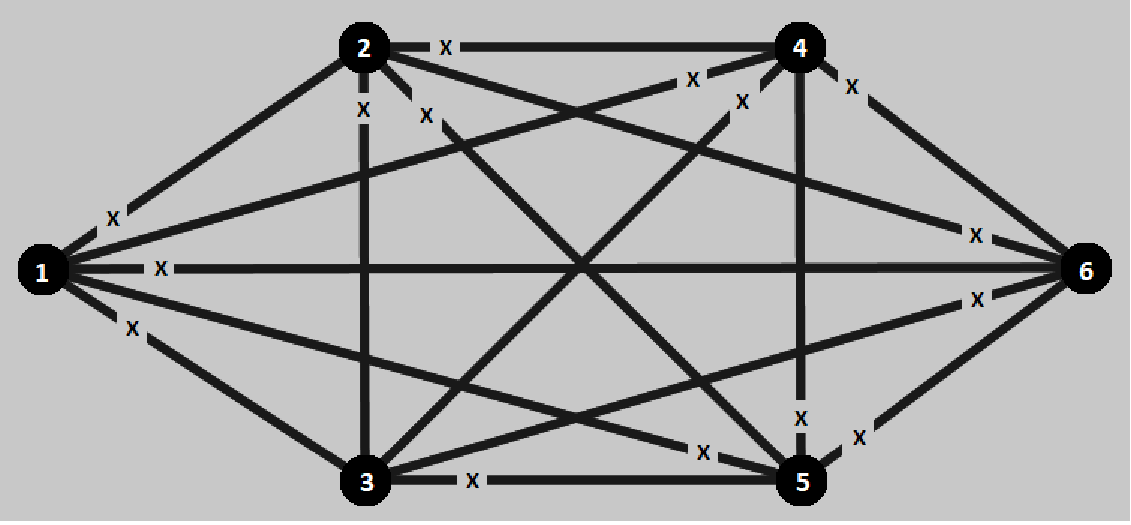
\includegraphics[width=13cm]{sdf/heuristic/transparent/figures/allowed_optical}
\caption{Allowed optical topology. The allowed optical topology is defined by the transport mode (transparent transport mode in this case). It is assumed that each connections between demands supports up to 100 lightpaths.}
\label{allowed_optical_surv_ref_low_heuristic_transparent}
\end{figure}

\begin{figure}[H]
\centering
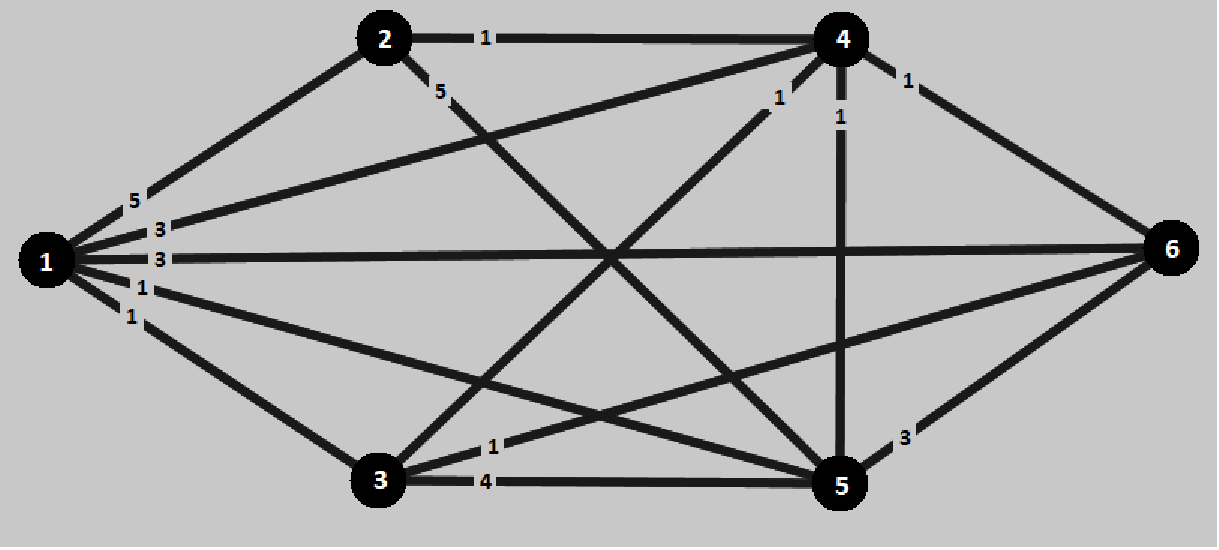
\includegraphics[width=13cm]{sdf/heuristic/transparent/figures/logical_topology_odu0_low}
\caption{ODU0 logical topology defined by the ODU0 traffic matrix.}
\label{logical_ODU0_surv_ref_low_heuristic_transparent}
\end{figure}

\begin{figure}[H]
\centering
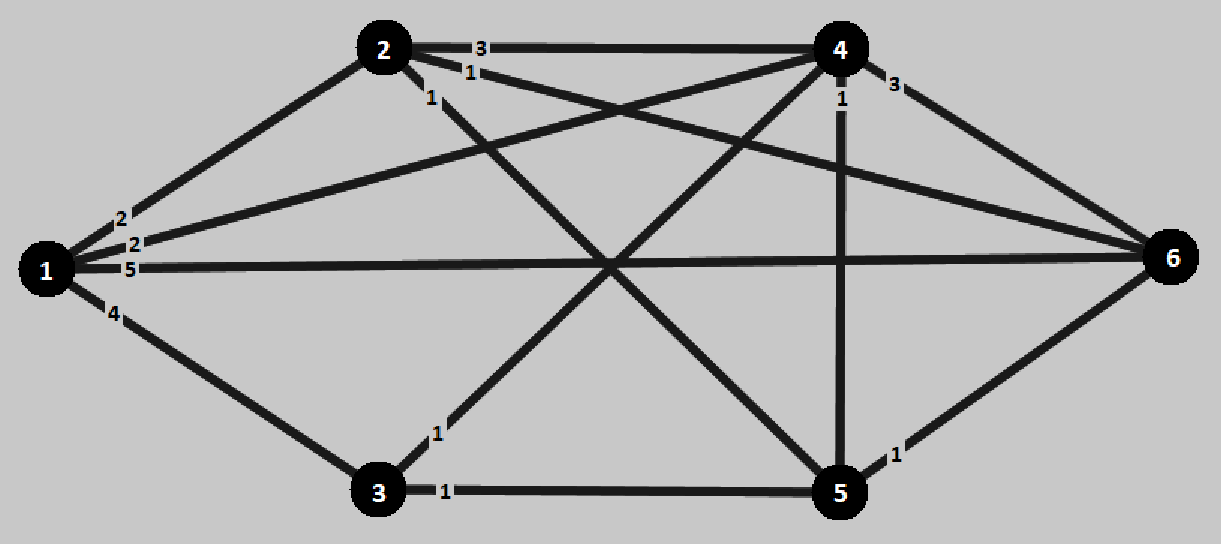
\includegraphics[width=13cm]{sdf/heuristic/transparent/figures/logical_topology_odu1_low}
\caption{ODU1 logical topology defined by the ODU1 traffic matrix.}
\label{logical_ODU1_surv_ref_low_heuristic_transparent}
\end{figure}

\begin{figure}[H]
\centering
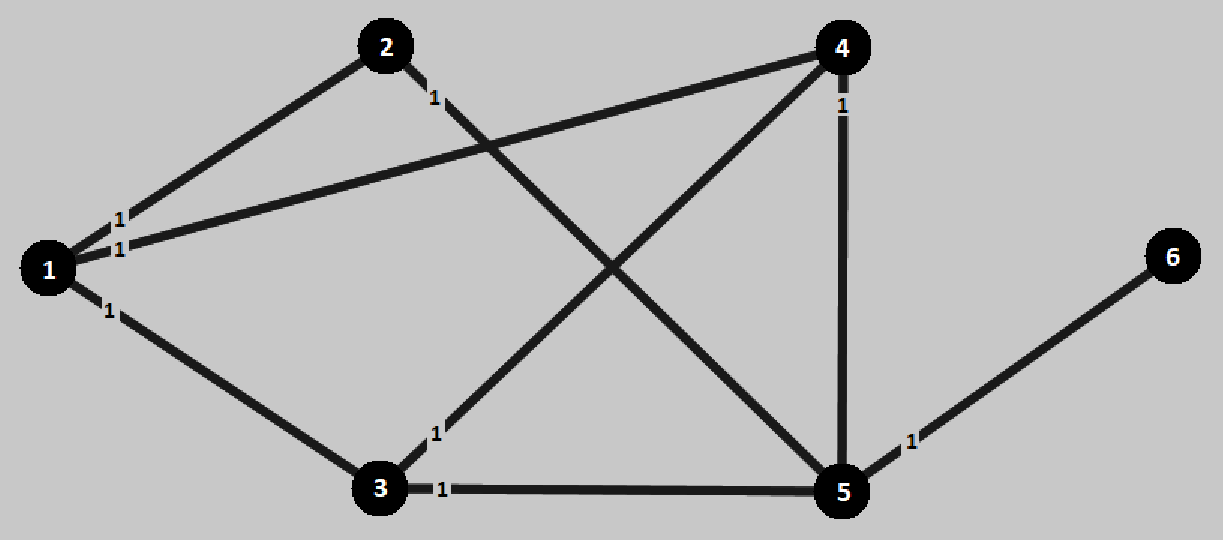
\includegraphics[width=13cm]{sdf/heuristic/transparent/figures/logical_topology_odu2_low}
\caption{ODU2 logical topology defined by the ODU2 traffic matrix.}
\label{logical_ODU2_surv_ref_low_heuristic_transparent}
\end{figure}

\begin{figure}[H]
\centering
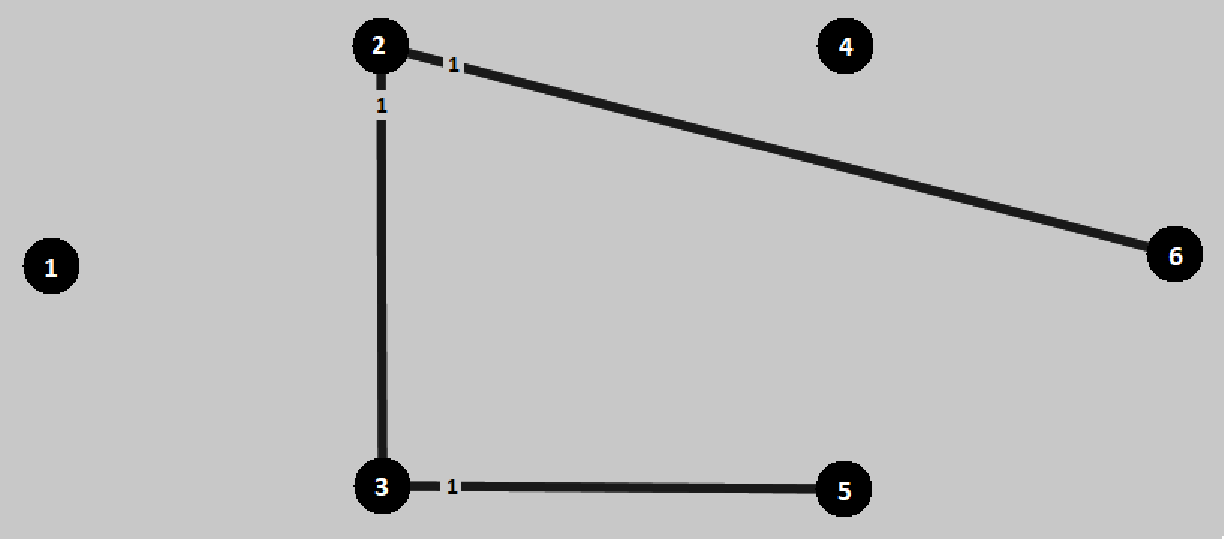
\includegraphics[width=13cm]{sdf/heuristic/transparent/figures/logical_topology_odu3_low}
\caption{ODU3 logical topology defined by the ODU3 traffic matrix.}
\label{logical_ODU3_surv_ref_low_heuristic_transparent}
\end{figure}

\begin{figure}[H]
\centering
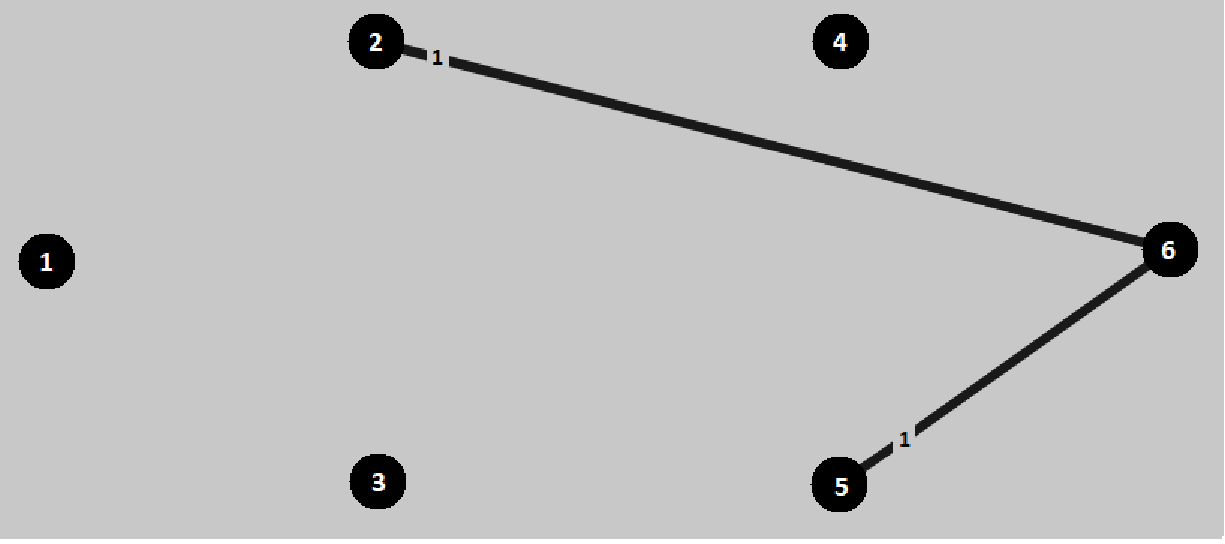
\includegraphics[width=13cm]{sdf/heuristic/transparent/figures/logical_topology_odu4_low}
\caption{ODU4 logical topology defined by the ODU4 traffic matrix.}
\label{logical_ODU4_surv_ref_low_heuristic_transparent}
\end{figure}

\begin{figure}[H]
\centering
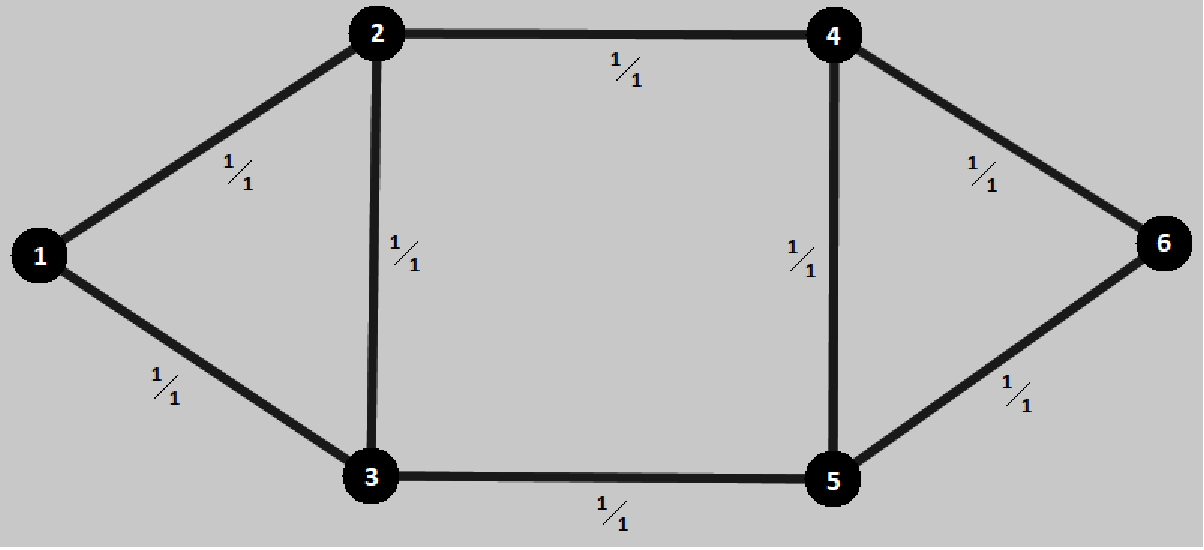
\includegraphics[width=13cm]{sdf/heuristic/transparent/figures/physical_topology}
\caption{Physical topology after dimensioning.}
\label{physical_topology_surv_ref_low_heuristic_transparent}
\end{figure}

Following all the steps mentioned in the \ref{net2plan_guide}, applying the routing and grooming heuristic algorithms in the Net2Plan software and using all the data referring to this scenario, the obtained result for the Vasco's heuristics can be consulted in the following table \ref{scripttransp_surv_ref_low_heuristic}.\\

\begin{table}[H]
\centering
\begin{tabular}{|| c | c | c | c | c | c | c ||}
 \hline
 \multicolumn{7}{|| c ||}{CAPEX of the Network} \\
 \hline
 \hline
 \multicolumn{3}{|| c |}{ } & Quantity & Unit Price & Cost & Total \\
 \hline
 \multirow{3}{*}{\makecell{Link \\ Cost}} & \multicolumn{2}{ c |}{OLTs} & 16 & 15 000 \euro & 240 000 \euro & \multirow{3}{*}{26 520 000 \euro} \\ \cline{2-6}
 & \multicolumn{2}{ c |}{100 Gbits/s Transceivers} & 52 & 5 000 \euro/Gbit/s & 26 000 000 \euro & \\ \cline{2-6}
 & \multicolumn{2}{ c |}{Amplifiers} & 70 & 4 000 \euro & 280 000 \euro & \\
 \hline
 \multirow{10}{*}{\makecell{Node \\ Cost}} & \multirow{7}{*}{Electrical} & EXCs & 6 & 10 000 \euro & 60 000 \euro & \multirow{10}{*}{3 797 590 \euro} \\ \cline{3-6}
  & & ODU0 Ports & 60 & 10 \euro/port & 600 \euro & \\ \cline{3-6}
 & & ODU1 Ports & 50 & 15 \euro/port & 750 \euro & \\ \cline{3-6}
 & & ODU2 Ports & 16 & 30 \euro/port & 480 \euro & \\ \cline{3-6}
 & & ODU3 Ports & 6 & 60 \euro/port & 360 \euro & \\ \cline{3-6}
 & & ODU4 Ports & 4 & 100 \euro/port & 400 \euro & \\ \cline{3-6}
 & & Transponders & 34 & 100 000 \euro/port & 3 400 000 \euro & \\ \cline{2-6}
 & \multirow{3}{*}{Optical} & OXCs & 6 & 20 000 \euro & 120 000 \euro & \\ \cline{3-6}
 & & Line Ports & 52 & 2 500 \euro/port & 130 000 \euro & \\ \cline{3-6}
 & & Add Ports & 34 & 2 500 \euro/port & 85 000 \euro & \\
 \hline
 \multicolumn{6}{|| c |}{Total Network Cost} & 30 317 590 \euro \\
\hline
\end{tabular}
\caption{Table with detailed description of CAPEX of Vasco's 2016 results.}
\label{scripttransp_surv_ref_low_heuristic}
\end{table}

\vspace{17pt}
All the values calculated in the previous table were obtained through the equations \ref{Capex_Link_heuristic} and \ref{Capex_Node_heuristic} referred to in section \ref{Heuristic_CAPEX}, but for a more detailed analysis we created table \ref{formulas_transp_heuristic} where we can see how all the parameters are calculated individually. \\

\begin{table}[h!]
\centering
\begin{tabular}{|| c | c ||}
 \hline
  & Equation used to calculate the cost \\ \hline
 OLTs & \(\displaystyle 2 \sum_{i=1}^{N}\sum_{j=i+1}^{N} L_{ij} \gamma_0^{OLT} \) \\ \hline
 Transceivers & \(\displaystyle 2 \sum_{i=1}^{N}\sum_{j=i+1}^{N} L_{ij} f_{ij}^{od} \gamma_1^{OLT} \tau \) \\ \hline
 Amplifiers & \(\displaystyle 2 \sum_{i=1}^{N}\sum_{j=i+1}^{N} L_{ij} N^R_{ij} c^R \) \\ \hline
 EXCs & \(\displaystyle \sum_{n=1}^N N_{exc,n} \gamma_{e0} \) \\ \hline
 ODU0 Port & \(\displaystyle \sum_{n=1}^{N} \sum_{d=1}^{N} N_{exc,n} D_{nd,0} \gamma_{e1,0} \) \\ \hline
 ODU1 Port & \(\displaystyle \sum_{n=1}^{N} \sum_{d=1}^{N} N_{exc,n} D_{nd,1} \gamma_{e1,1} \) \\ \hline
 ODU2 Port & \(\displaystyle \sum_{n=1}^{N} \sum_{d=1}^{N} N_{exc,n} D_{nd,2} \gamma_{e1,2} \)\\ \hline
 ODU3 Port & \(\displaystyle \sum_{n=1}^{N} \sum_{d=1}^{N} N_{exc,n} D_{nd,3} \gamma_{e1,3} \) \\ \hline
 ODU4 Port & \(\displaystyle \sum_{n=1}^{N} \sum_{d=1}^{N} N_{exc,n} D_{nd,4} \gamma_{e1,4} \) \\ \hline
 LR Transponders & \(\displaystyle \sum_{n=1}^{N} \sum_{j=1}^{N} N_{exc,n} \lambda_{od} \gamma_{e1,-1} \) \\ \hline
 OXCs & \(\displaystyle \sum_{n=1}^N N_{oxc,n} \gamma_{o0} \) \\ \hline
 Add Port & \(\displaystyle \sum_{n=1}^{N} \sum_{j=1}^{N} N_{oxc,n} \lambda_{od} \gamma_{o1} \) \\ \hline
 Line Port & \(\displaystyle \sum_{n=1}^{N} \sum_{j=1}^{N} N_{oxc,n} f_{ij}^{od} \gamma_{o1} \) \\ \hline
 CAPEX & The final cost is calculated by summing all previous results. \\
 \hline
 \end{tabular}
\caption{Table with description of calculation}
\label{formulas_transp_heuristic}
\end{table}

\noindent
\textbf{Medium Traffic Scenario:}\\

In this scenario we have to take into account the traffic calculated in \ref{medium_traffic_scenario}. In a first phase we will show the various existing topologies of the network. The first are the allowed topologies, physical and optical topologies, the second are the logical topology for all ODUs and finally the resulting physical topology.\\

\begin{figure}[H]
\centering
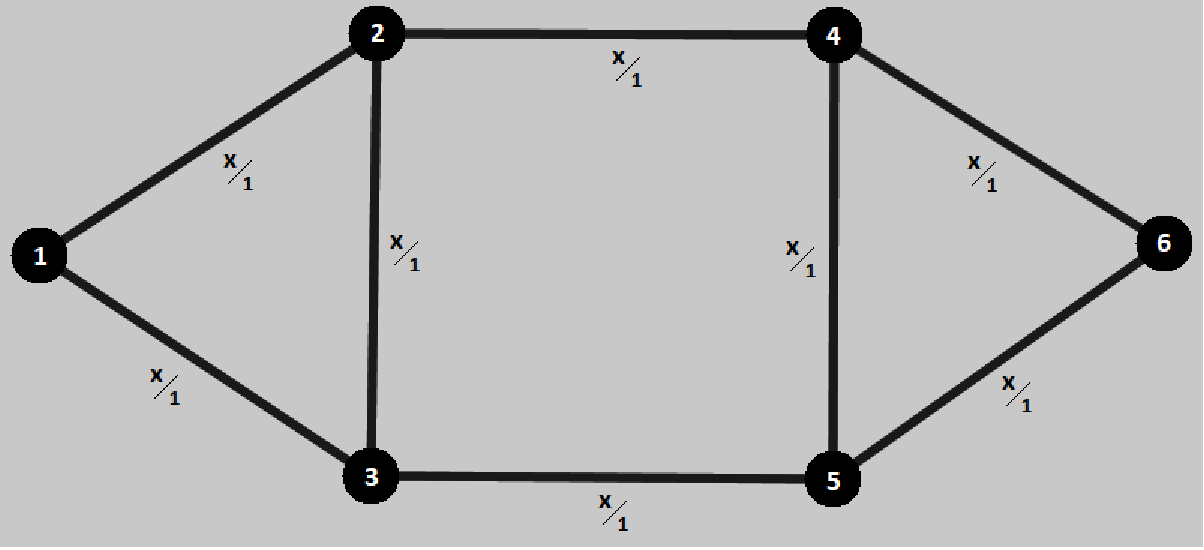
\includegraphics[width=13cm]{sdf/heuristic/transparent/figures/allowed_physical}
\caption{Allowed physical topology. The allowed physical topology is defined by the duct and sites in the field. It is assumed that each duct supports up to 1 bidirectional transmission system and each site supports up to 1 node.}
\label{allowed_physical_surv_ref_medium_heuristic_transparent}
\end{figure}

\begin{figure}[H]
\centering
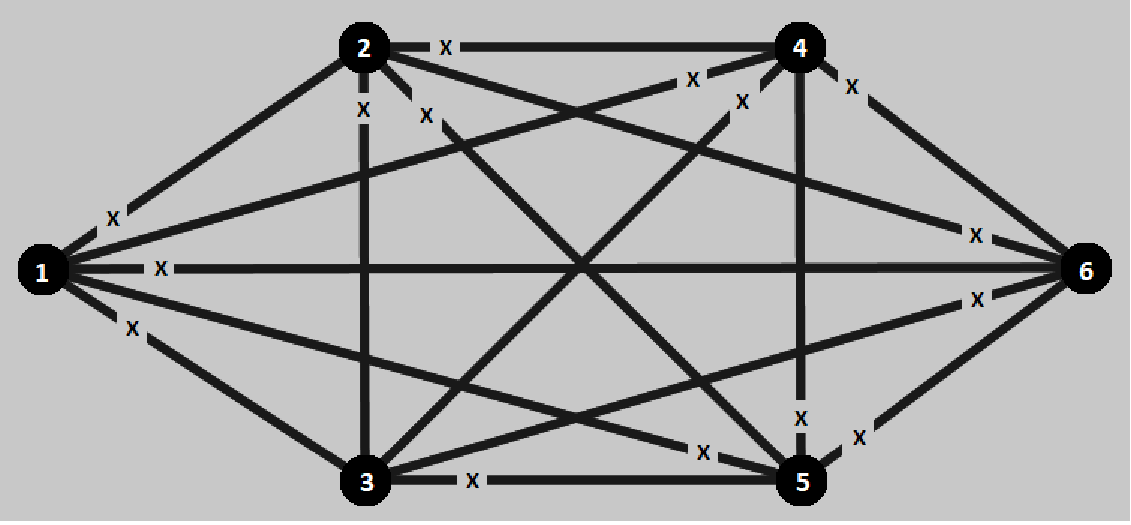
\includegraphics[width=13cm]{sdf/heuristic/transparent/figures/allowed_optical}
\caption{Allowed optical topology. The allowed optical topology is defined by the transport mode (transparent transport mode in this case). It is assumed that each connections between demands supports up to 100 lightpaths.}
\label{allowed_optical_surv_ref_medium_heuristic_transparent}
\end{figure}

\begin{figure}[H]
\centering
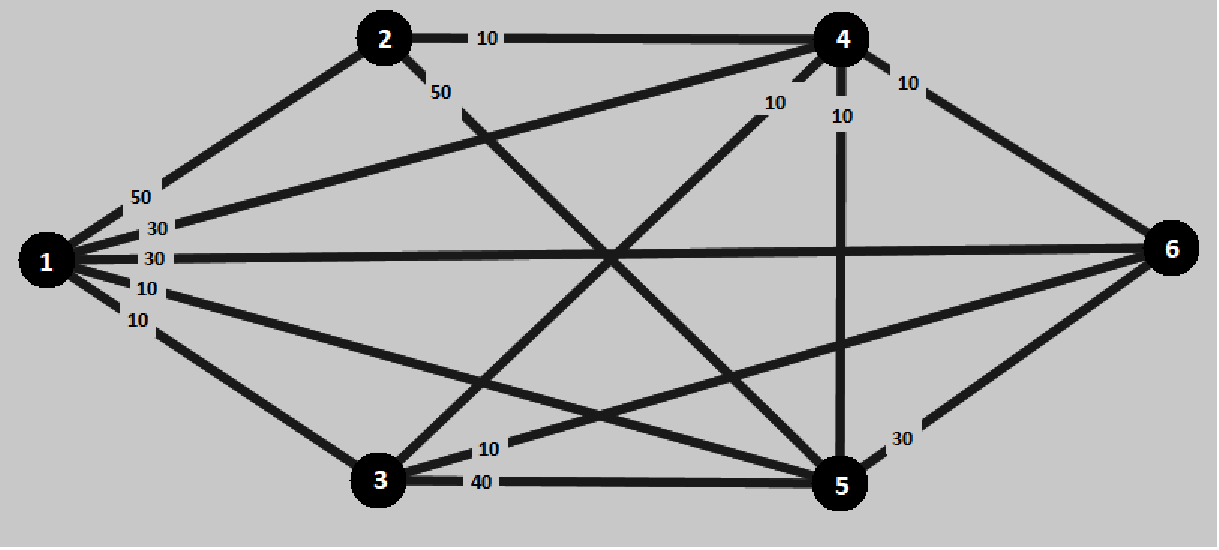
\includegraphics[width=13cm]{sdf/heuristic/transparent/figures/logical_topology_odu0_medium}
\caption{ODU0 logical topology defined by the ODU0 traffic matrix.}
\label{logical_ODU0_surv_ref_medium_heuristic_transparent}
\end{figure}

\begin{figure}[H]
\centering
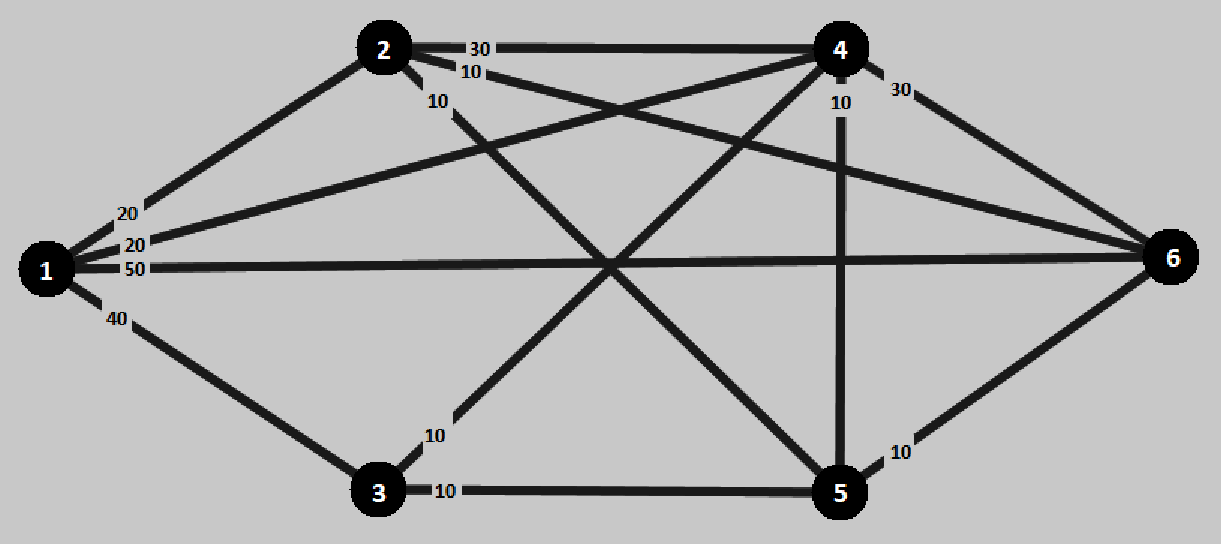
\includegraphics[width=13cm]{sdf/heuristic/transparent/figures/logical_topology_odu1_medium}
\caption{ODU1 logical topology defined by the ODU1 traffic matrix.}
\label{logical_ODU1_surv_ref_medium_heuristic_transparent}
\end{figure}

\begin{figure}[H]
\centering
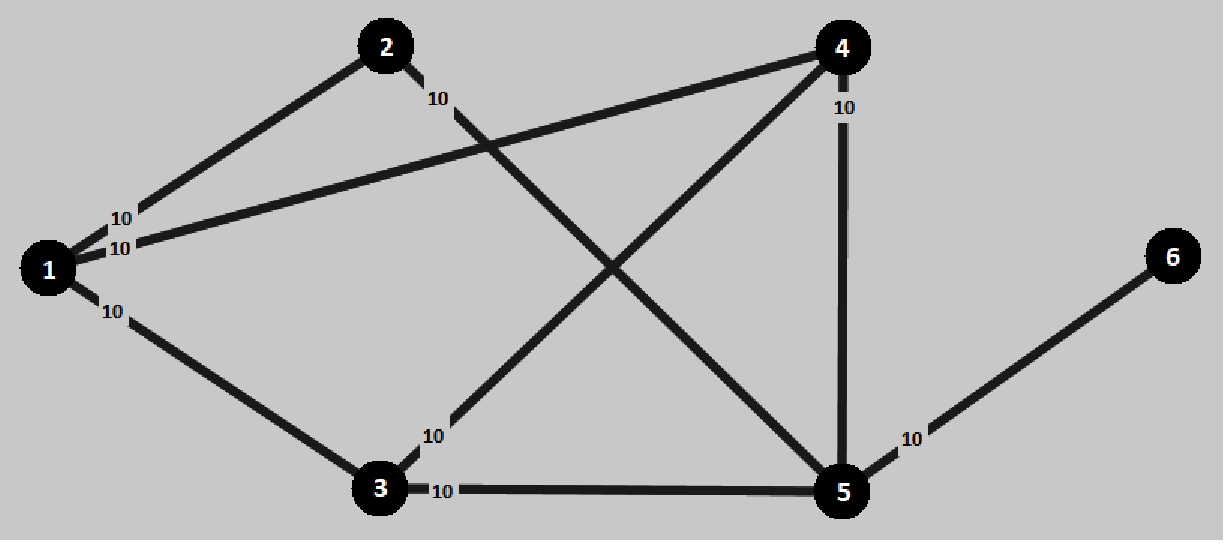
\includegraphics[width=13cm]{sdf/heuristic/transparent/figures/logical_topology_odu2_medium}
\caption{ODU2 logical topology defined by the ODU2 traffic matrix.}
\label{logical_ODU2_surv_ref_medium_heuristic_transparent}
\end{figure}

\begin{figure}[H]
\centering
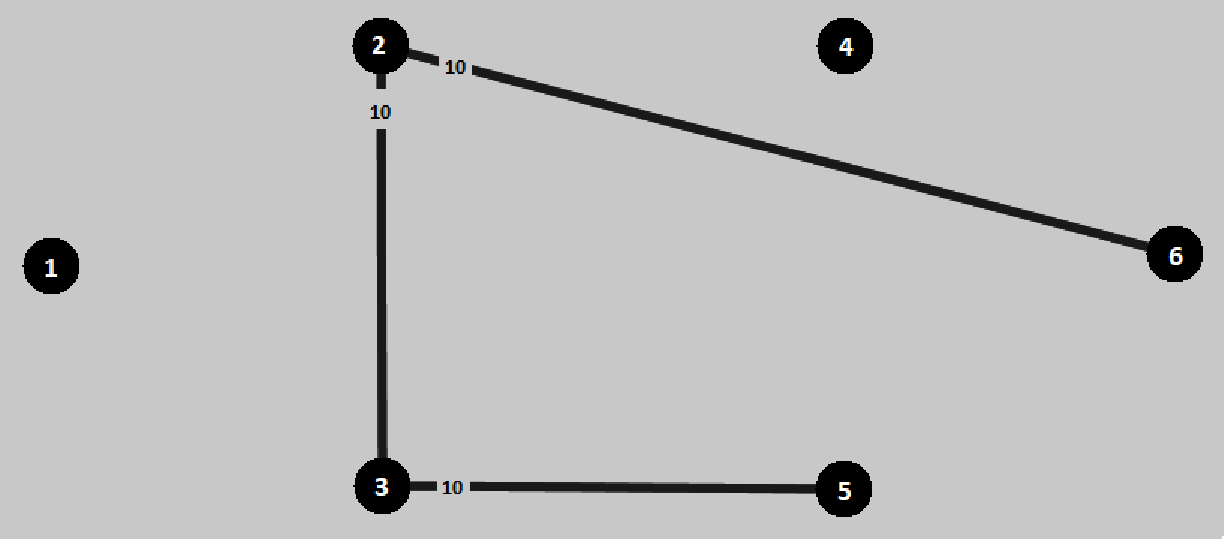
\includegraphics[width=13cm]{sdf/heuristic/transparent/figures/logical_topology_odu3_medium}
\caption{ODU3 logical topology defined by the ODU3 traffic matrix.}
\label{logical_ODU3_surv_ref_medium_heuristic_transparent}
\end{figure}

\begin{figure}[H]
\centering
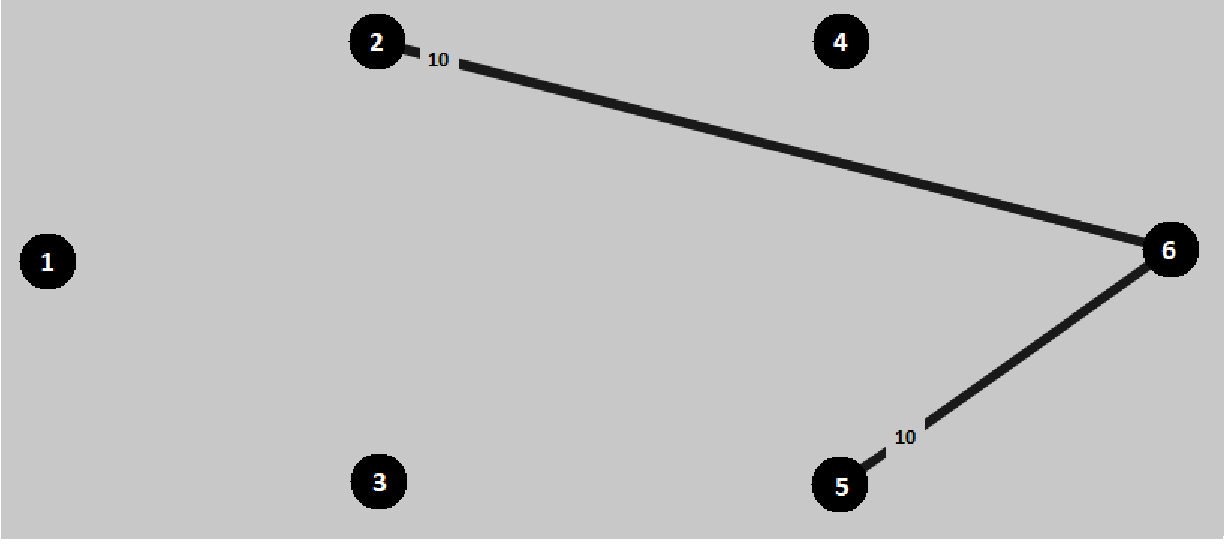
\includegraphics[width=13cm]{sdf/heuristic/transparent/figures/logical_topology_odu4_medium}
\caption{ODU4 logical topology defined by the ODU4 traffic matrix.}
\label{logical_ODU4_surv_ref_medium_heuristic_transparent}
\end{figure}

\begin{figure}[H]
\centering
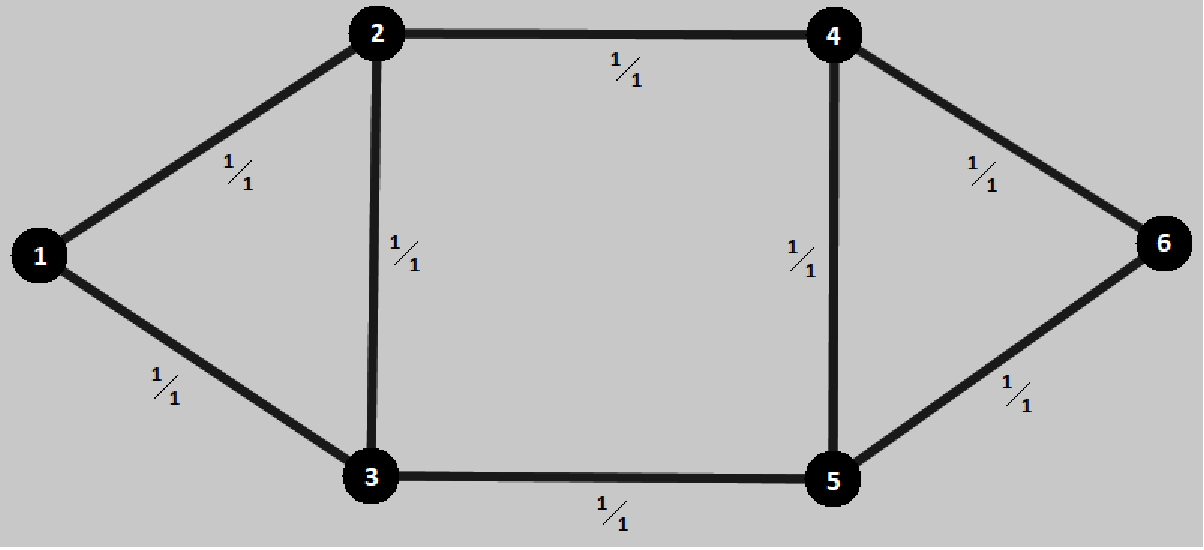
\includegraphics[width=13cm]{sdf/heuristic/transparent/figures/physical_topology}
\caption{Physical topology after dimensioning.}
\label{physical_topology_surv_ref_medium_heuristic_transparent}
\end{figure}

Following all the steps mentioned in the \ref{net2plan_guide}, applying the routing and grooming heuristic algorithms in the Net2Plan software and using all the data referring to this scenario, the obtained result for the Vasco's heuristics can be consulted in the following table \ref{scripttransp_surv_ref_medium_heuristic}. In table \ref{formulas_transp_heuristic} mentioned in previous scenario we can see how all the values were calculated. \\

\begin{table}[H]
\centering
\begin{tabular}{|| c | c | c | c | c | c | c ||}
 \hline
 \multicolumn{7}{|| c ||}{CAPEX of the Network} \\
 \hline
 \hline
 \multicolumn{3}{|| c |}{ } & Quantity & Unit Price & Cost & Total \\
 \hline
 \multirow{3}{*}{\makecell{Link \\ Cost}} & \multicolumn{2}{ c |}{OLTs} & 16 & 15 000 \euro & 240 000 \euro & \multirow{3}{*}{84 520 000 \euro} \\ \cline{2-6}
 & \multicolumn{2}{ c |}{100 Gbits/s Transceivers} & 168 & 5 000 \euro/Gbit/s & 84 000 000 \euro & \\ \cline{2-6}
 & \multicolumn{2}{ c |}{Amplifiers} & 70 & 4 000 \euro & 280 000 \euro & \\
 \hline
 \multirow{10}{*}{\makecell{Node \\ Cost}} & \multirow{7}{*}{Electrical} & EXCs & 6 & 10 000 \euro & 60 000 \euro & \multirow{10}{*}{15 180 900 \euro} \\ \cline{3-6}
 & & ODU0 Ports & 600 & 10 \euro/port & 6 000 \euro & \\ \cline{3-6}
 & & ODU1 Ports & 500 & 15 \euro/port & 7 500 \euro & \\ \cline{3-6}
 & & ODU2 Ports & 160 & 30 \euro/port & 4 800 \euro & \\ \cline{3-6}
 & & ODU3 Ports & 60 & 60 \euro/port & 3 600 \euro & \\ \cline{3-6}
 & & ODU4 Ports & 40 & 100 \euro/port & 4 000 \euro & \\ \cline{3-6}
 & & Transponders & 142 & 100 000 \euro/port & 14 200 000 \euro & \\ \cline{2-6}
 & \multirow{3}{*}{Optical} & OXCs & 6 & 20 000 \euro & 120 000 \euro & \\ \cline{3-6}
 & & Line Ports & 168 & 2 500 \euro/port & 420 000 \euro & \\ \cline{3-6}
 & & Add Ports & 142 & 2 500 \euro/port & 355 000 \euro & \\
 \hline
 \multicolumn{6}{|| c |}{Total Network Cost} & 99 700 900 \euro \\
\hline
\end{tabular}
\caption{Table with detailed description of CAPEX of Vasco's 2016 results.}
\label{scripttransp_surv_ref_medium_heuristic}
\end{table}

\noindent
\textbf{High Traffic Scenario:}\\

In this scenario we have to take into account the traffic calculated in \ref{high_traffic_scenario}. In a first phase we will show the various existing topologies of the network. The first are the allowed topologies, physical and optical topologies, the second are the logical topology for all ODUs and finally the resulting physical topology.\\

\begin{figure}[H]
\centering
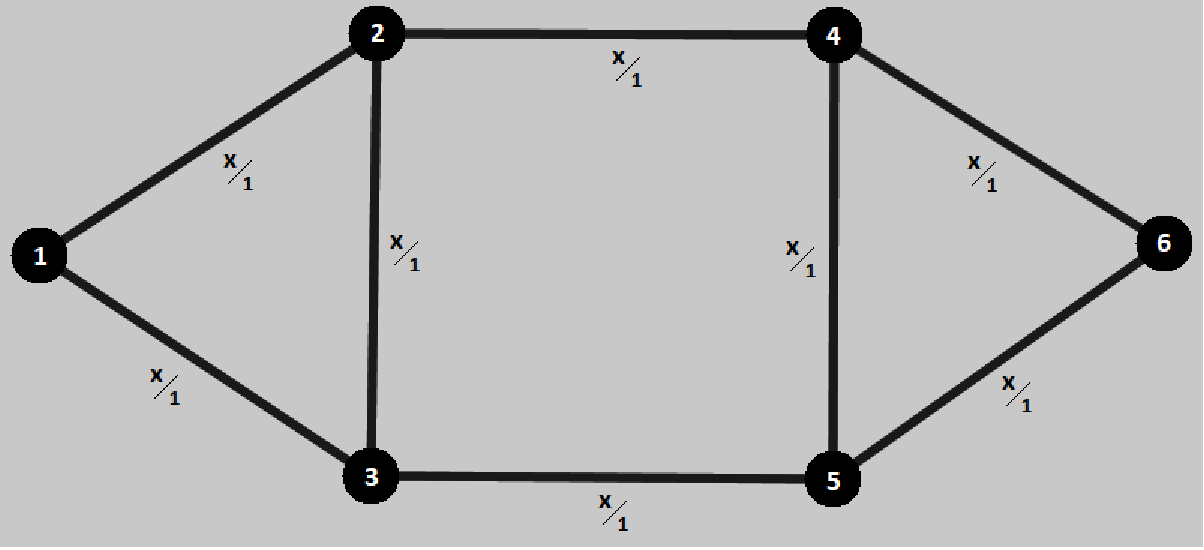
\includegraphics[width=13cm]{sdf/heuristic/transparent/figures/allowed_physical}
\caption{Allowed physical topology. The allowed physical topology is defined by the duct and sites in the field. It is assumed that each duct supports up to 1 bidirectional transmission system and each site supports up to 1 node.}
\label{allowed_physical_surv_ref_high_heuristic_transparent}
\end{figure}

\begin{figure}[H]
\centering
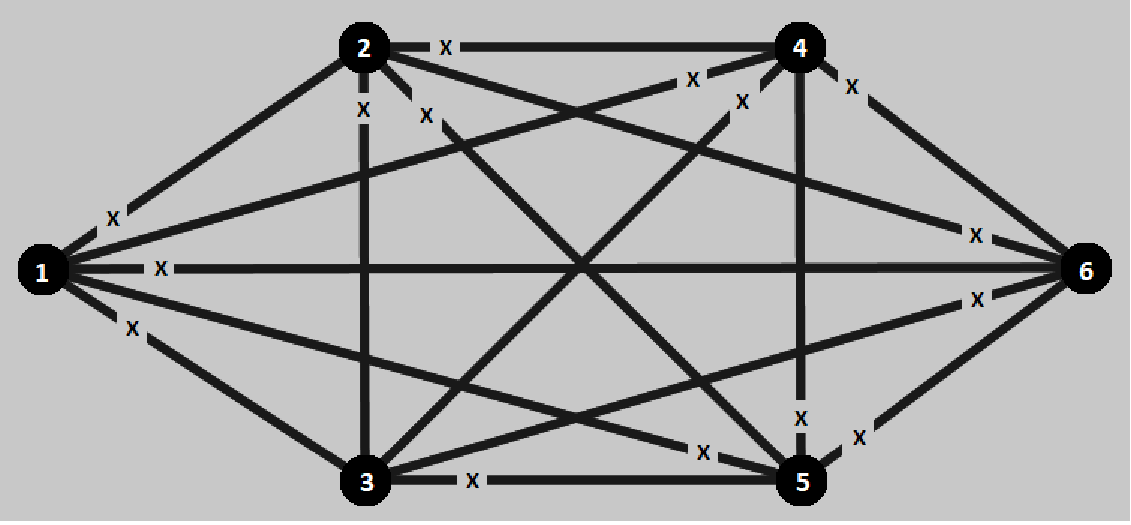
\includegraphics[width=13cm]{sdf/heuristic/transparent/figures/allowed_optical}
\caption{Allowed optical topology. The allowed optical topology is defined by the transport mode (transparent transport mode in this case). It is assumed that each connections between demands supports up to 100 lightpaths.}
\label{allowed_optical_surv_ref_high_heuristic_transparent}
\end{figure}

\begin{figure}[H]
\centering
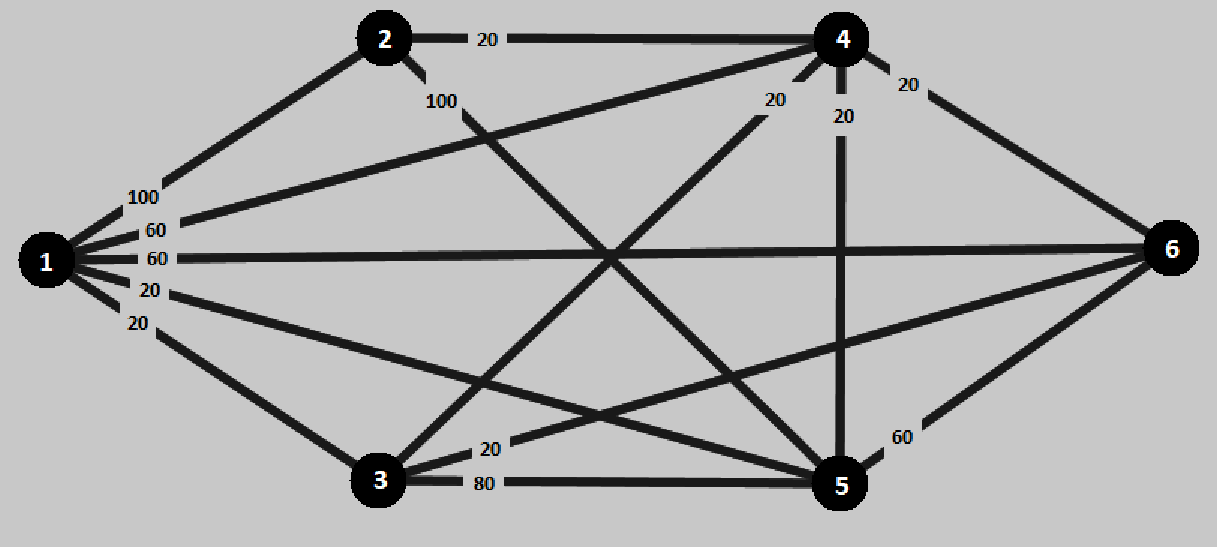
\includegraphics[width=13cm]{sdf/heuristic/transparent/figures/logical_topology_odu0_high}
\caption{ODU0 logical topology defined by the ODU0 traffic matrix.}
\label{logical_ODU0_surv_ref_high_heuristic_transparent}
\end{figure}

\begin{figure}[H]
\centering
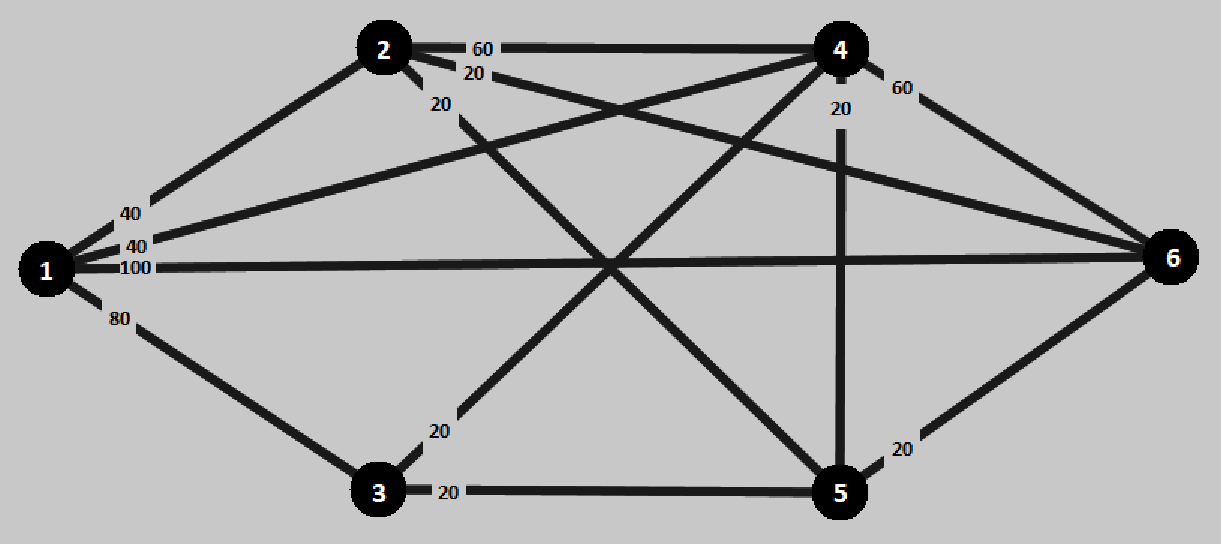
\includegraphics[width=13cm]{sdf/heuristic/transparent/figures/logical_topology_odu1_high}
\caption{ODU1 logical topology defined by the ODU1 traffic matrix.}
\label{logical_ODU1_surv_ref_high_heuristic_transparent}
\end{figure}

\begin{figure}[H]
\centering
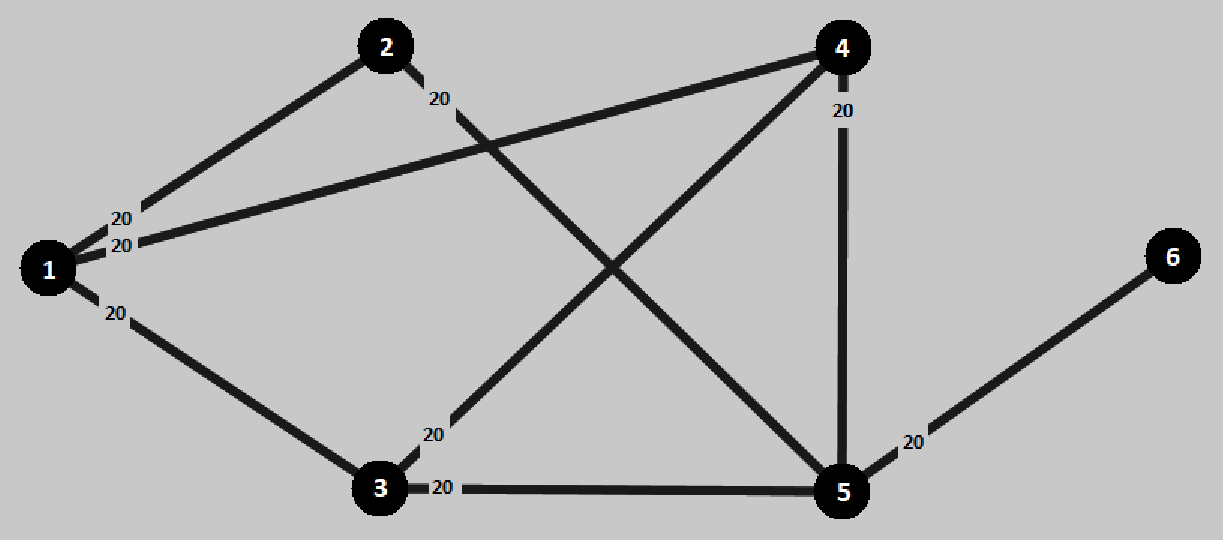
\includegraphics[width=13cm]{sdf/heuristic/transparent/figures/logical_topology_odu2_high}
\caption{ODU2 logical topology defined by the ODU2 traffic matrix.}
\label{logical_ODU2_surv_ref_high_heuristic_transparent}
\end{figure}

\begin{figure}[H]
\centering
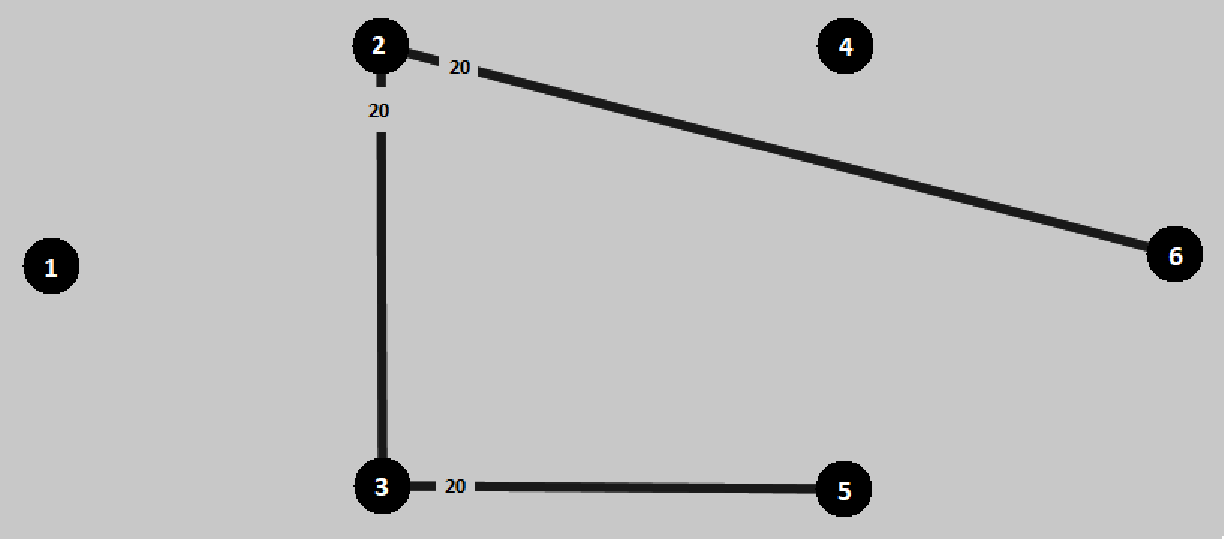
\includegraphics[width=13cm]{sdf/heuristic/transparent/figures/logical_topology_odu3_high}
\caption{ODU3 logical topology defined by the ODU3 traffic matrix.}
\label{logical_ODU3_surv_ref_high_heuristic_transparent}
\end{figure}

\begin{figure}[H]
\centering
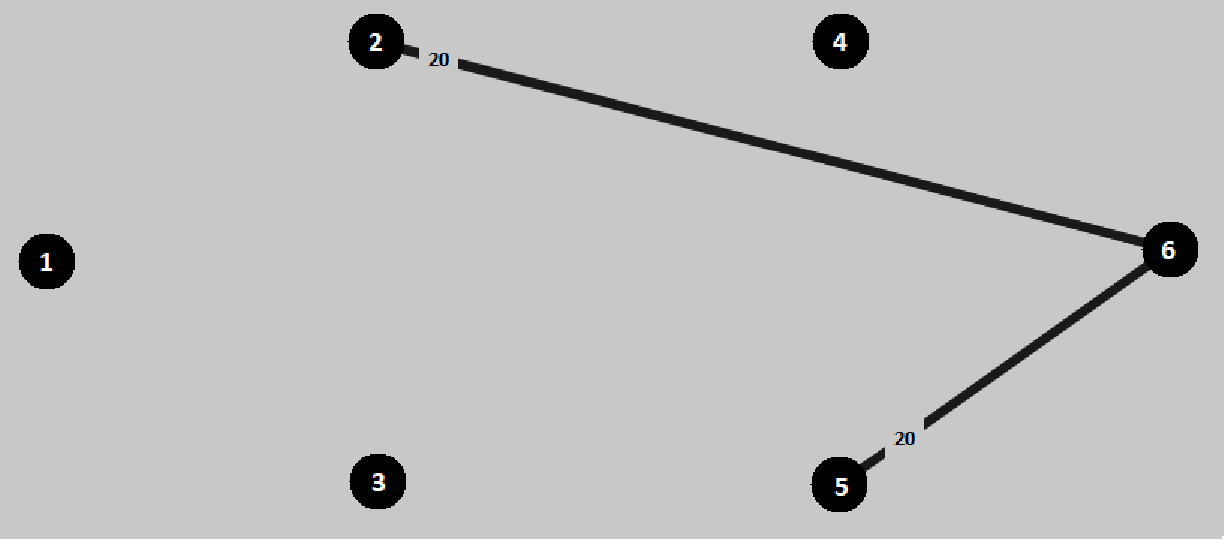
\includegraphics[width=13cm]{sdf/heuristic/transparent/figures/logical_topology_odu4_high}
\caption{ODU4 logical topology defined by the ODU4 traffic matrix.}
\label{logical_ODU4_surv_ref_high_heuristic_transparent}
\end{figure}

\begin{figure}[H]
\centering
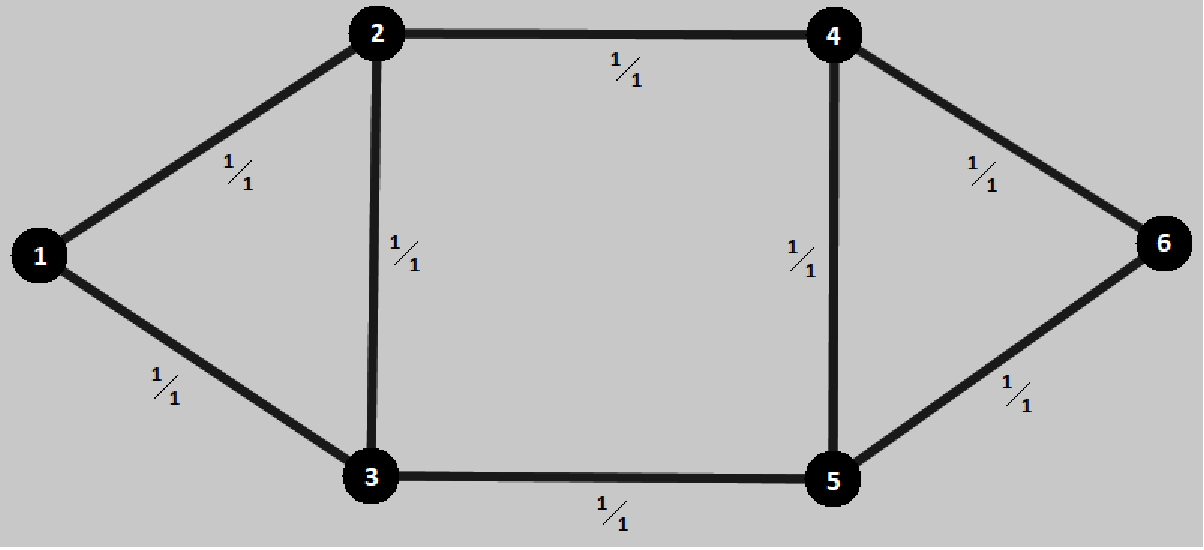
\includegraphics[width=13cm]{sdf/heuristic/transparent/figures/physical_topology}
\caption{Physical topology after dimensioning.}
\label{physical_topology_surv_ref_high_heuristic_transparent}
\end{figure}

Following all the steps mentioned in the \ref{net2plan_guide}, applying the routing and grooming heuristic algorithms in the Net2Plan software and using all the data referring to this scenario, the obtained result for the Vasco's heuristics can be consulted in the following table \ref{scripttransp_surv_ref_high_heuristic}. In table \ref{formulas_transp_heuristic} mentioned in previous scenario we can see how all the values were calculated. \\

\begin{table}[H]
\centering
\begin{tabular}{|| c | c | c | c | c | c | c ||}
 \hline
 \multicolumn{7}{|| c ||}{CAPEX of the Network} \\
 \hline
 \hline
 \multicolumn{3}{|| c |}{ } & Quantity & Unit Price & Cost & Total \\
 \hline
 \multirow{3}{*}{\makecell{Link \\ Cost}} & \multicolumn{2}{ c |}{OLTs} & 16 & 15 000 \euro & 240 000 \euro & \multirow{3}{*}{157 520 000 \euro} \\ \cline{2-6}
 & \multicolumn{2}{ c |}{100 Gbits/s Transceivers} & 314 & 5 000 \euro/Gbit/s & 157 000 000 \euro & \\ \cline{2-6}
 & \multicolumn{2}{ c |}{Amplifiers} & 70 & 4 000 \euro & 280 000 \euro & \\
 \hline
 \multirow{10}{*}{\makecell{Node \\ Cost}} & \multirow{7}{*}{Electrical} & EXCs & 6 & 10 000 \euro & 60 000 \euro & \multirow{10}{*}{28 486 800 \euro} \\ \cline{3-6}
  & & ODU0 Ports & 1 200 & 10 \euro/port & 12 000 \euro & \\ \cline{3-6}
 & & ODU1 Ports & 1 000 & 15 \euro/port & 15 000 \euro & \\ \cline{3-6}
 & & ODU2 Ports & 320 & 30 \euro/port & 9 600 \euro & \\ \cline{3-6}
 & & ODU3 Ports & 120 & 60 \euro/port & 7 200 \euro & \\ \cline{3-6}
 & & ODU4 Ports & 80 & 100 \euro/port & 8 000 \euro & \\ \cline{3-6}
 & & Transponders & 268 & 100 000 \euro/port & 26 800 000 \euro & \\ \cline{2-6}
 & \multirow{3}{*}{Optical} & OXCs & 6 & 20 000 \euro & 120 000 \euro & \\ \cline{3-6}
 & & Line Ports & 314 & 2 500 \euro/port & 785 000 \euro & \\ \cline{3-6}
 & & Add Ports & 268 & 2 500 \euro/port & 670 000 \euro & \\
 \hline
 \multicolumn{6}{|| c |}{Total Network Cost} & 186 006 800 \euro \\
\hline
\end{tabular}
\caption{Table with detailed description of CAPEX of Vasco's 2016 results.}
\label{scripttransp_surv_ref_high_heuristic}
\end{table}

\vspace{13pt}
\subsubsection{Conclusions}

Once we have obtained the results for all the scenarios we will now draw some conclusions about these results. For a better analysis of the results will be created the table \ref{table_comparative_transp_surv_heuristic} with the number of line ports, tributary ports and transceivers because they are important values for the cost of CAPEX, the cost of links, the cost of nodes and finally the cost of CAPEX.\\

\begin{table}[H]
\centering
\begin{tabular}{| c | c | c | c |}
 \hline
   & Low Traffic & Medium Traffic  & High Traffic \\
 \hline\hline
 Traffic (Gbit/s) & 500 & 5 000 & 10 000 \\ \hline
 Bidirectional Links used & 8 & 8 & 8 \\ \hline
 Number of Add ports & 34 & 142 & 268 \\ \hline
 Number of Line ports & 52 & 168 & 314 \\ \hline
 Number of Tributary ports & 136 & 1 360 & 2 720 \\ \hline
 Number of Transceivers & 52 & 168 & 314 \\ \hline
 Link Cost & 26 520 000 \euro & 84 520 000 \euro & 157 520 000 \euro \\ \hline
 Node Cost & 3 797 590 \euro & 15 180 900 \euro & 28 486 800 \euro \\ \hline
 CAPEX & \textbf{30 317 590 \euro} & \textbf{99 700 900 \euro} & \textbf{186 006 800 \euro} \\ \hline
 CAPEX/Gbit/s & \textbf{60 635 \euro/Gbit/s} & \textbf{19 940 \euro/Gbit/s} & \textbf{18 600 \euro/Gbit/s} \\ \hline
\end{tabular}
\caption{Table with different value of CAPEX for this case.}
\label{table_comparative_transp_surv_heuristic}
\end{table}

\noindent
Looking at the previous table we can make some comparisons between the several scenario:

\begin{itemize}
  \item Comparing the low traffic with the others we can see that despite having an increase of factor ten (medium traffic) and factor twenty (high traffic), the same increase does not occur in the final cost (it is lower);
  \subitem This happens because the number of the transceivers is lower than expected which leads by carrying the traffic with less network components and, consequently, the network CAPEX is lower;
  \item Comparing the medium traffic with the high traffic we can see that the increase of the factor is double and in the final cost this factor is very close but still inferior;
  \subitem This happens because the number of the transceivers is also lower but very close to the expected;
  \item Comparing the CAPEX cost per bit we can see that in the low traffic the cost is higher than the medium and high traffic, which in these two cases the value is similar, but still inferior in the higher traffic;
  \subitem This happens because the lower the traffic, the higher CAPEX/bit will be. We can see that in medium and high traffic the results tend to be one closer and lower value.
\end{itemize}

\vspace{13pt}
\subsubsection{Opens Issues}

The creation of this model for any scenario, started with some considerations and some open issues being:

\begin{itemize}
  \item Allow blocking.
  \subitem The presented model assume that the solution is possible or impossible, does not support a partial solution where some demands are not routed (are blocked);
  \item Allow multiple transmission system.
  \subitem The presented model for each link only supports one transmission system.
\end{itemize}


\newpage
\vspace{11pt}

\chapter{Transparent transport mode}

\begin{tcolorbox}	
	\begin{tabular}{p{2.75cm} p{0.2cm} p{10.5cm}} 	
		\textbf{Student Name}   &:& Eduardo Fernandes    (09/11/2018 - )\\
		\textbf{Goal}           &:& Allows blocking, i.e., creation of a model that supports a partial solution where some demands are not routed (are blocked).
	\end{tabular}
\end{tcolorbox}

 \vspace{11pt}
 In figure 1.112 a top level diagram is presented in which it is represented the heuristcs approach implemented behind the developed algorithms. %Next on figure on figure xxx2 the same diagram is presented but in a lower level approach with more detailed information related to the so called super blocks, those that perform more complex functions.

\begin{figure}[H]
	\centering
	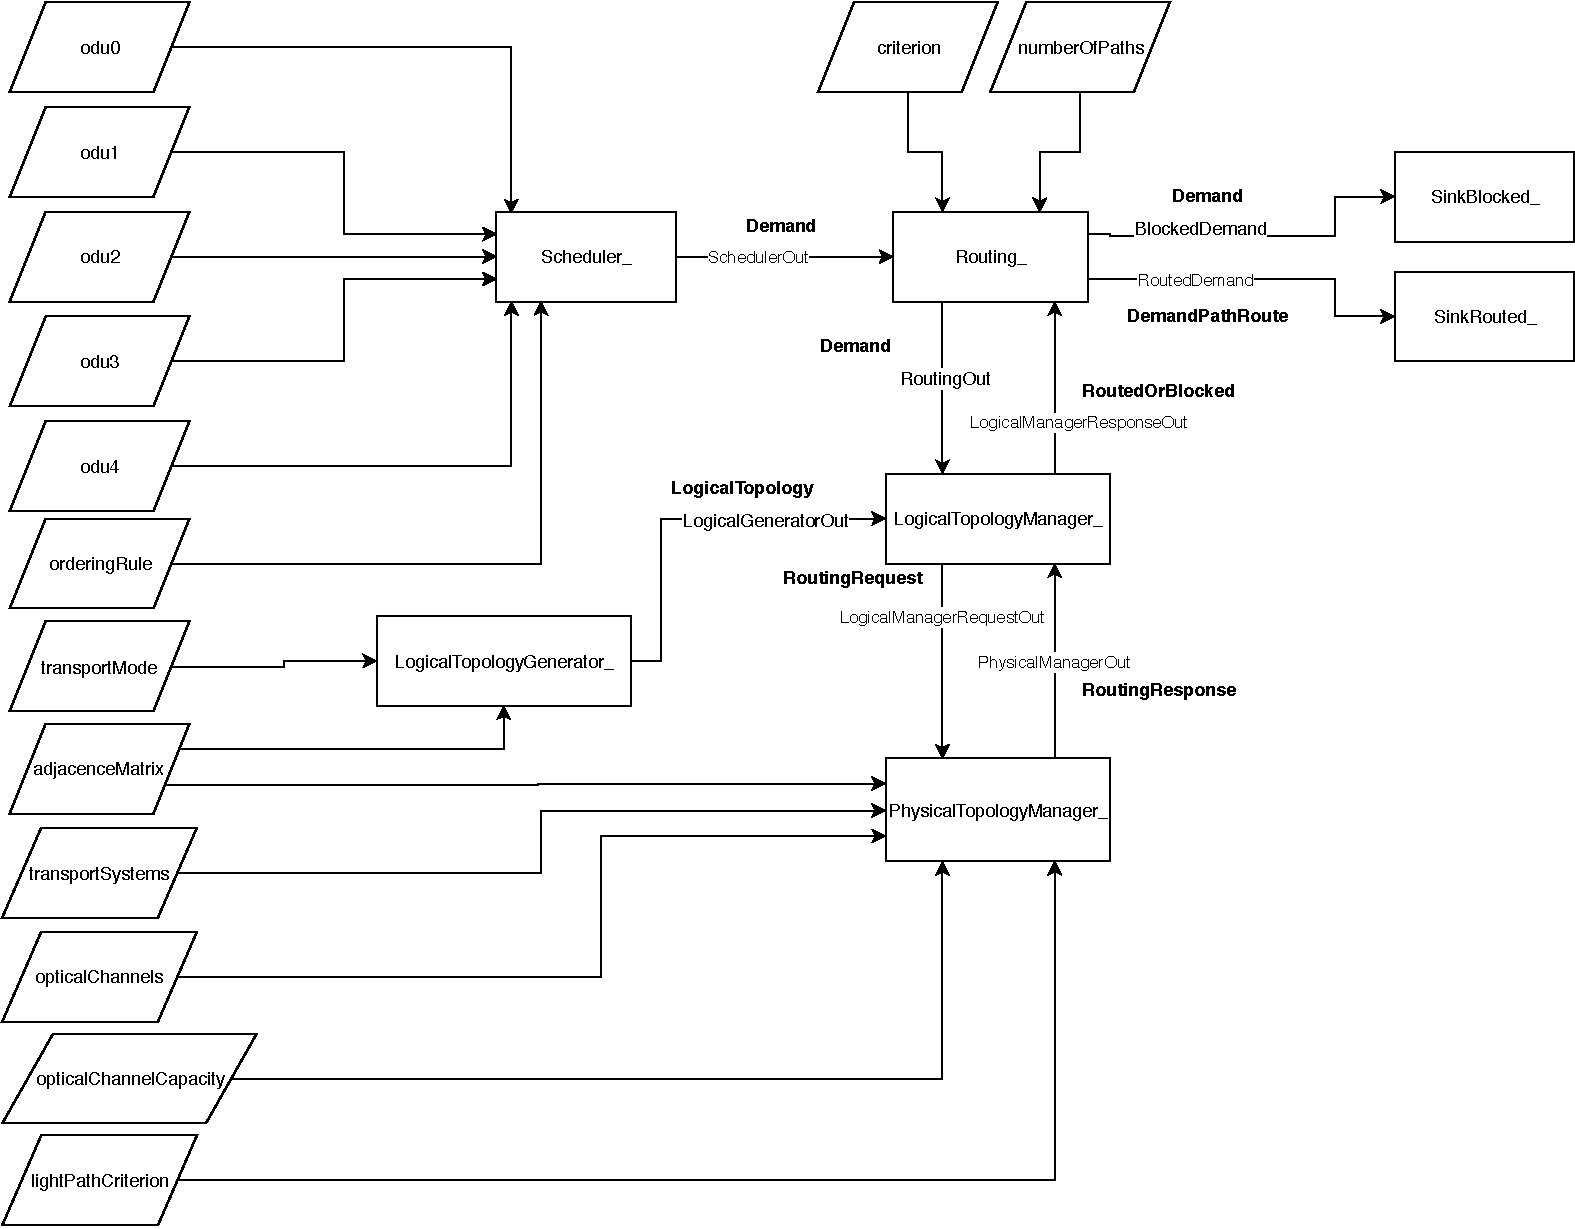
\includegraphics[width=15cm]{sdf/heuristic/transparent/figures/novoFluxograma}
	\caption{High level diagram of the heuristic algorithm performed.}
	\label{fluxogram_transparent_surv}
\end{figure}

\section{Concepts}
This section serves to introduce some of the terminology used throughout the dissertation.
\subsection{Network Nodes} 
The circles in the network graphs presented above represent nodes, these are points in the network that terminate and switch traffic.
\subsection{Network Links}
The lines connecting network nodes can be mentioned both as physical links or optical multiplexing systems and they are tipically depicted with just a single line and are formed by one fiber that carries traffic in a certain direction. 

\section{System inputs}
\begin{table}[H]
	\centering
	\begin{tabular}{|c|c|c|}
		\hline
		\textbf{Parameter} & \textbf{Default value} & \textbf{Description}                                                                                           \\ \hline
		numberOfNodes & 0 & Number of existing nodes in the network. \\ \hline
		odu0                                                                         & [0]          & N by N matrix containing ODU0 demands.                                                                                     \\ \hline
		odu1                                                                         & [0]          & N by N matrix containing ODU1 demands.                                                                                        \\ \hline
		odu2                                                                         & [0]          &N by N matrix containing ODU2 demands.                                                                                        \\ \hline
		odu3                                                                         & [0]          & N by N matrix containing ODU3 demands.                                                                                        \\ \hline
		odu4                                                                         & [0]          & N by N matrix containing ODU4 demands.                                                                                        \\ \hline
		orderingRule                                                        & descendingOrder   & \begin{tabular}[c]{@{}l@{}}descendingOrder (ODU4 to ODU0)\\ ascendingOrder (ODU0 to ODU4)\end{tabular} \\ \hline
		transportMode                                                               & transparent          & \begin{tabular}[c]{@{}c@{}}"opaque", "transparent" or "translucent".\end{tabular}                   \\ \hline
		physicalTopologyAdjacencyMatrix                                                            & [0]          & \begin{tabular}[c]{@{}c@{}}Physical connections of the\\ network.\end{tabular}                       \\ \hline
		numberOfOMSPerLink                                                            & 1             & \begin{tabular}[c]{@{}c@{}}Number of optical multiplexing systems\\ existing in each physical link.\end{tabular} \\ \hline
		numberOfOpticalChannelsPerOMS                                                             & 100           & \begin{tabular}[c]{@{}c@{}}Number of optical channels per\\ optical multiplexing system\end{tabular}                    \\ \hline
		initialWavelenght & 1550 & \begin{tabular}[c]{@{}c@{}}Initial value of the wavelenght used \\ expressed in nanometers (nm).\end{tabular} \\ \hline
		wavelenghtSpacing & 0.8 & Interval  between used wavlenghts (nm). \\ \hline
		\begin{tabular}[c]{@{}c@{}}opticalChannelCapacity\end{tabular}           & 100 Gbps      & \begin{tabular}[c]{@{}c@{}}Physical capacity of each \\ optical channel.\end{tabular}                        \\ \hline
		routingCriterionLogicalTopology                                                                    & Hops          & Shortest path type.                                                                                  \\             \hline
		routingCriterionPhysicalTopology                                                                    & Hops          & Shortest path type.                                                                                  \\             \hline
		blockingCriterionLogicalTopology                                                              & 3             & \begin{tabular}[c]{@{}c@{}}Number of attempted paths \\ before blocking a demand.\end{tabular}                      \\  \hline
		blockingCriterionPhysicalTopology                                                              & 3             & \begin{tabular}[c]{@{}c@{}}Number of attempts before\\ discarding a possible path.\end{tabular}                      \\  \hline                                                       
	\end{tabular}
	\caption{System input parameters.}
	\label{system_input}
\end{table}
%\Large Summary explanation \\ \\

%\normalsize As it is shown in \ref{fluxogram_transparent_surv}, it is needed a Scheduler\_  block which will be responsible for the creation of an ordered queue containing all the demands entering this network, in an order previously defined (based on the demands ODU type), and ready to be routed.
%In order to route those demands there will also be the necessity of a PathGenerator\_  block which as its own name implies will create a list of the shortest logical paths for each demand between its source and destination nodes, through information received by the LogicalTopologyGenerator\_  block. Next, in the PathTester\_  block the list of paths previously associated to a demand are tested in order to check their availability in terms of physical and grooming capacity in each of the necessary links that comprise the light path used. A LogicalTopologyGenerator\_  and a PhysicalTopologyGenerator\_  are then also needed, the first in order to create the matrix of possible logical connections between nodes and the structure of each of those logical links, and the other to create structures for every physical links which in turn are constituded by many optical channels. Both will further on be continuously updated in the PathTester\_  block. Finally, there are two remaining Sink blocks one to store demands that were routed (SinkRouted\_ ) and their correspondent information and the other to register blocked demands (SinkBlocking\_ ). Both are very useful to store the information that will later on be present in the final cost report.\\\\
%Knowing the list of possible shortest logical paths associated to a demand (through Dijkstra algotithm), the capacity of the physical links that constitute those logical connections have to be tested. That will occur in the next block of the diagram, the PathTester\_  block.\\ \\ \\

%If there is already an entry in the light path table and if the remaining capacity of that light path, already established, is sufficient to route the demand then our demand is added to that same light path and a demandPathRoute signal is created with information regarding to the demand/path index, route and wavelength used by that same demand. If on the other side the logical path being tested has not enough capacity to process a certain demand or if there is no light path established between that pair of source and destination nodes than an attempt to create another light path entry will be made. If it occurs successfully than a new light path is established in our network and the demand is routed through that same but if there is no possibility of creating a new light path between those nodes than our logical path will have to be ignored and cutted of, and so a next shortest logical path must be tested in the same manner. In order to in further iterations that full path not be considered a path type signal (RemovedPaths) should be created to inform the Path Generator block that those paths must not be considered, this will make the algorithm more efficient. If finally we can not route our demand though none of the logical paths selected then a blocking state occurs, the demand is not routed and a demandsBlocked signal is created. Then finally a cost report is created to obtain a detailed estimation of the network Capex based on user defined equipment costs present on table 1.28.\\ \\


%\begin{figure}[H]
%	\centering
%	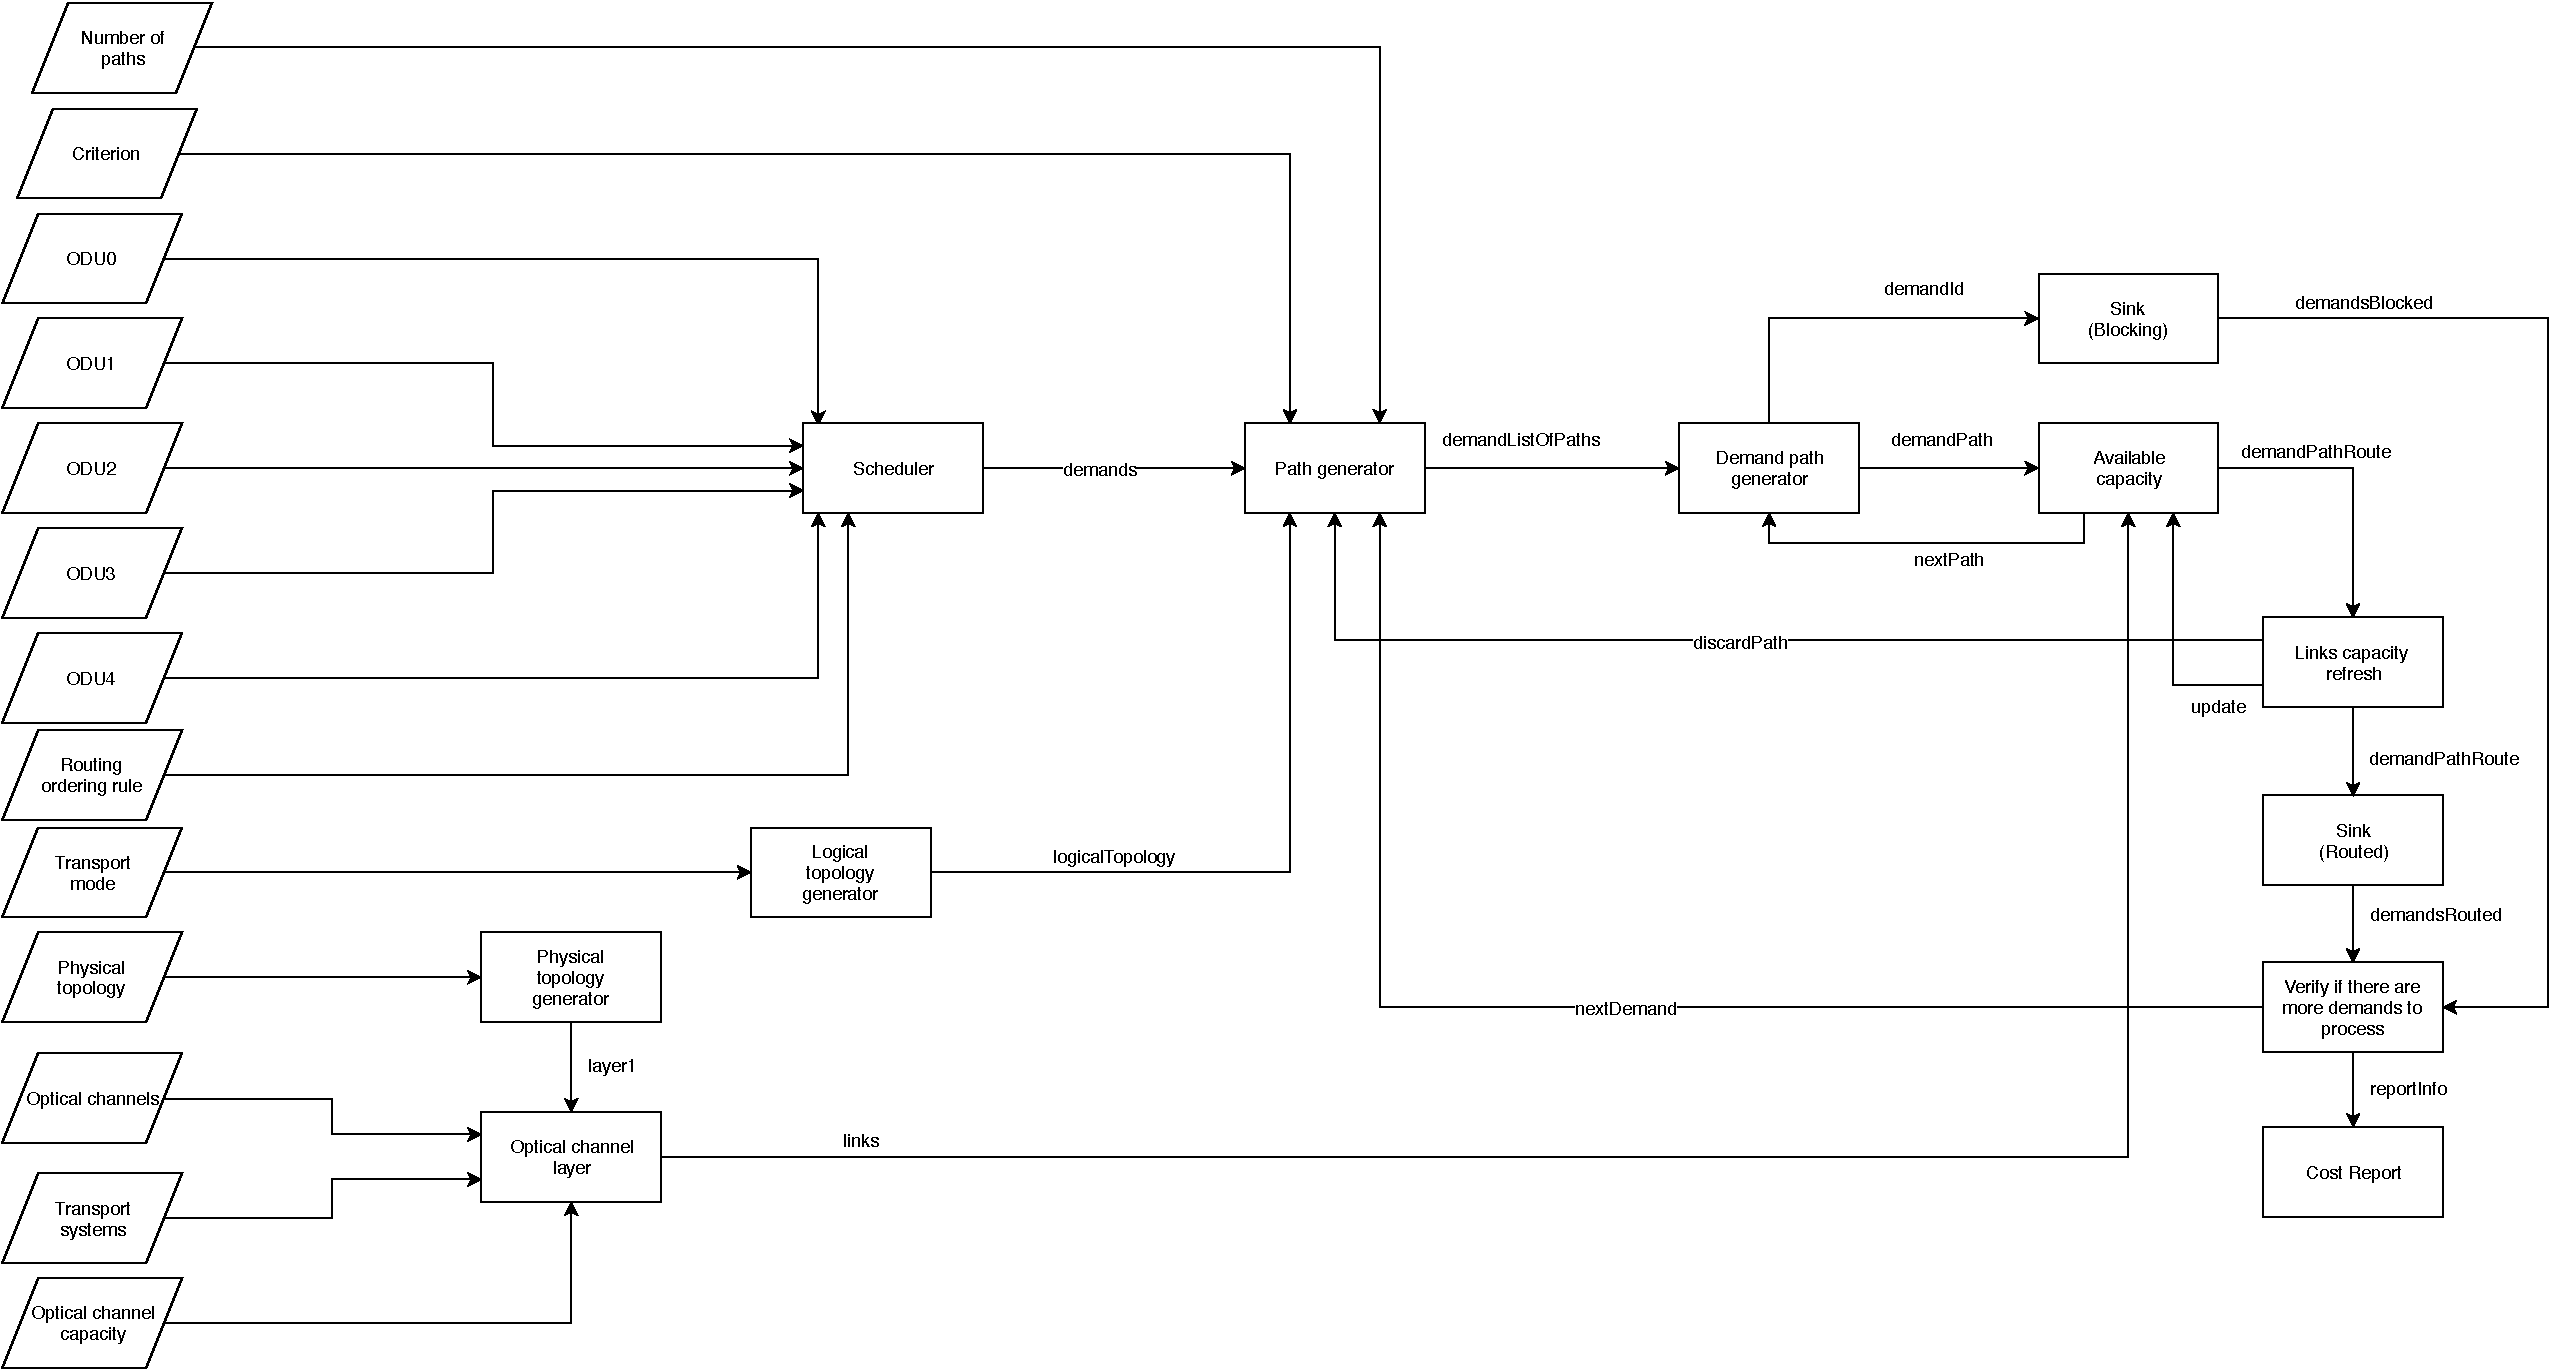
\includegraphics[width=16cm]{sdf/heuristic/transparent/figures/fluxogramaSemGrooming}
%	\caption{Low level diagram of the algorithms performed.}
%	\label{fluxogram_transparent_surv}
%\end{figure}

%Here the main difference is the decomposition of the two super blocks 'Path tester' which is divided in three sub blocks ('Demand path generator', 'Available capacity' and 'Link capacity refresh') and the 'Physical Topology generator' block, divided in two other blocks, all of this in order to better understand their exact functions.

\section{System signals}

\begin{table}[H]
	\centering
	\begin{tabular}{| c | c | c |}
		\hline
		 \textbf{Signal name} &  \textbf{Signal type} \\ % it is missing the description of the signals
		\hline
		Scheduler\_Out &  DemandRequest\\ \hline
		LogicalTopologyGenerator\_Out &  LogicalTopology\\ \hline
		PhysicalTopologyGenerator\_Out & PhysicalTopology\\ \hline
		LogicalTopologyManager\_PathRequest & PathRequest\\ \hline
		PhysicalTopologyManager\_PathRequestRouted & PathRequestRouted\\ \hline
		ProcessedDemand &  DemandRequestRouted\\ \hline
		FinalLogicalTopology & LogicalTopology\\ \hline
		FinalPhysicalTopology & PhysicalTopology\\ \hline
	\end{tabular}
	\caption{System Signals.}
	\label{system_signals}
\end{table}
	Table \ref{system_signals} presents the system signals as well as their type.\\ \\

\section{Type signals structures}

\subsection{LogicalTopology}

The logical topology of the network is an approach that defines how components are connected. Each node may be optical directly connected to each other, or only optical connected to adjacent nodes or optical connected to suitable nodes. These possibilities are demostrated below on table \ref{logical_topology}, where 0/1 indicates the possibility of establishing a logical connection between nodes.\\ 

Below are represented the variables that constitute a LogicalTopology type signal.\\ \\
\textbf{logicalTopologyMatrix}
\begin{table}[H]
	\centering	
	\begin{tabular}{|c|c|c|ccc|c|}
		\hline
		\textbf{Nodes} & 1 & 2 & \multicolumn{3}{c|}{...} & N \\ \hline
		1 & \textbf{0} & 0/1 & \multicolumn{3}{c|}{...} & 0/1 \\ \hline
		2 & 0/1 & \textbf{0} & \multicolumn{3}{c|}{...} & 0/1 \\ \hline
		\textbf{.} & \textbf{.} & \textbf{.} & \textbf{.} &  &  & \textbf{.} \\
		\textbf{.} & \textbf{.} & \textbf{.} &  & \textbf{.} &  & \textbf{.} \\
		\textbf{.} & \textbf{.} & \textbf{.} &  &  & \textbf{.} & \textbf{.} \\ \hline
		N & 0/1 & 0/1 & \multicolumn{3}{c|}{...} & \textbf{0} \\ \hline
	\end{tabular}
	\caption{Allowed logical topology for a matrix of N nodes.}
	\label{physical_topology}
\end{table}
N represents the number of nodes present in the network.\\ \\
Therefore, these shorter optical paths along the route imposed by logical topology lead to a situation of three possible transport modes: Opaque, Transparent and Translucent. During this dissertation the focus will be on transparent models, where each node connects to all others creating direct links between all nodes of the network.\\ \\


The next variables are distributed in an hierarchical mode, a Path consists in one or more Light Paths which in its turn are formed by one or more Optical Channels.\\ \\
\textbf{paths}
\begin{table}[H]
	\centering
	\begin{tabular}{|c|c|c|c|c|c|}
		\hline
		pathIndex & sourceNode & destinationNode & \begin{tabular}[c]{@{}c@{}}capacity\\ (ODU0s)\end{tabular} & numberOfLightPaths & lightPathsIndex \\ \hline
		0 or greater & 1...N & 1...N & 0...80 & 0 or greater & {[}lp\_1, lp\_2, ...{]} \\ \hline
	\end{tabular}
	\caption{Structure of a path variable.}
	\label{path}
\end{table}

\textbf{lightPaths}
\begin{table}[H]
	\centering
\begin{tabular}{|c|c|c|c|c|c|}
	\hline
	lightPathIndex & sourceNode & destinationNode & \begin{tabular}[c]{@{}c@{}}capacity\\ (ODU0s)\end{tabular} & \begin{tabular}[c]{@{}c@{}}numberOfOptical-\\ Channels\end{tabular} & \begin{tabular}[c]{@{}c@{}}opticalChannels-\\ Index\end{tabular} \\ \hline
	0 or greater & 1...N & 1...N & 0..80 & 0 or greater & {[}och\_1, och\_2,...{]} \\ \hline
\end{tabular}
	\caption{Structure of a light path variable.}
	\label{lightPath}
\end{table}

\textbf{opticalChannels}

\begin{table}[H]
	\centering
\begin{tabular}{|c|c|c|c|c|c|c|}
	\hline
	\begin{tabular}[c]{@{}c@{}}opticalChannel-\\ Index\end{tabular} & sourceNode & \begin{tabular}[c]{@{}c@{}}destination-\\ Node\end{tabular} & \begin{tabular}[c]{@{}c@{}}capacity\\ (ODU0s)\end{tabular} &  \begin{tabular}[c]{@{}c@{}}wavelenght\\ (nm)\end{tabular} & \begin{tabular}[c]{@{}c@{}}numberOf-\\ Demands\end{tabular} & \begin{tabular}[c]{@{}c@{}}demands-\\ Index\end{tabular} \\ \hline
	0 or greater & 1...N & 1...N & 0...80 & {[}to define{]} & 0 or greater & {[}d\_1, ...{]} \\ \hline
\end{tabular}
	\caption{Structure of an optical channel variable.}
	\label{opticalChannels}
\end{table}

If the network starts with no initial information or files given then these three last variables will be created and sent to the LogicalTopologyManager\_  block void, where later on will be updated. 
%\begin{table}[H]
%	\centering
%	\begin{tabular}{|c|c|c|c|c|}
%		\hline
%		Link Index & Light Path Number & Physical Links  & Wavelenght & Capacity (ODU0s) \\ \hline
%		1          & 1                 & {[}0/1...0/1{]} & 1...OC     &                  \\ \hline
%		...        & ...               & ...             & ...        &                  \\ \hline
%		LO         & LP                & {[}0/1...0/1{]} & 1...OC     &                  \\ \hline
%	\end{tabular}
%	\caption{Light path variable.}
%	\label{lightpath_example}
%\end{table}
%LP represents the number of light paths established in the network.\\
%OC represents the number optical channels existent in each physical link.\\
%The Physical Links variable inside of the light paths represents the links existent in our network, in this case they can assume two different values, 0 or 1, depending on whether they are used or not to route a demand through a certain light path.\\ \\
\subsection{PhysicalTopology}

The physical topology can be seen as a layout of a real optical network. The allowed physical topology is defined by the duct and sites in the field. It is assumed that each duct supports up to 2 unidirectional  optical multiplexing systems, that will behave like a bidirectional connection between a pair of nodes, and each site supports up to 1 node.\\ \\

Below are represented the variables that constitute a PhysicalTopology type signal.\\ \\
\textbf{physicalTopologyMatrix}
\begin{table}[H]
	\centering	
	\begin{tabular}{|c|c|c|ccc|c|}
		\hline
		\textbf{Nodes} & 1 & 2 & \multicolumn{3}{c|}{...} & N \\ \hline
		1 & \textbf{0} & 0/1 & \multicolumn{3}{c|}{...} & 0/1 \\ \hline
		2 & 0/1 & \textbf{0} & \multicolumn{3}{c|}{...} & 0/1 \\ \hline
		\textbf{.} & \textbf{.} & \textbf{.} & \textbf{.} &  &  & \textbf{.} \\
		\textbf{.} & \textbf{.} & \textbf{.} &  & \textbf{.} &  & \textbf{.} \\
		\textbf{.} & \textbf{.} & \textbf{.} &  &  & \textbf{.} & \textbf{.} \\ \hline
		N & 0/1 & 0/1 & \multicolumn{3}{c|}{...} & \textbf{0} \\ \hline
	\end{tabular}
	\caption{Allowed physical topology for a matrix of N nodes.}
	\label{physical_topology}
\end{table}
0/1 indicates the possibility of existing a physical connection between nodes.\\ \\

Based on the previous adjacence matrix a data structure is created for each of the unidirectional optical multiplexing systems interconnecting nodes.\\ \\
\textbf{opticalMultiplexingSystems}\\
\begin{table}[H]
	\centering
	\begin{tabular}{|c|c|c|c|c|c|}
		\hline
		\begin{tabular}[c]{@{}c@{}}opticalMultiplexing-\\ SystemIndex\end{tabular} & sourceNode & \begin{tabular}[c]{@{}c@{}}destination-\\ Node\end{tabular} & \begin{tabular}[c]{@{}c@{}}numberOf-\\ Wavelenghts\end{tabular} & wavelenghts & \begin{tabular}[c]{@{}c@{}}available-\\ Wavelenghts\end{tabular} \\ \hline
		0 & 1...N & 1...N & OC & {[}w\_1, w\_2, ...{]} & {[}0/1 ... 0/1{]} \\ \hline
		... & ... & ... & ... & ... & ... \\ \hline
		L-1 & 1...N & 1...N & OC & {[}w\_1, w\_2, ...{]} & {[}0/1 ... 0/1{]} \\ \hline
	\end{tabular}
	\caption{Structure of the opticalMultiplexingSystems variables.}
	\label{PhysicalGeneratorOut}
\end{table}

OC represents the number of optical channels present in a physical link.\\
L represent the total number of existent unidirectional physical links in the network.\\
w\_1 and w\_2 represent values of possible wavelengths to be used.\\
In the availableWavelenghts array 0/1 dictates if the corresponding wavelenght value of wavelenghts array is available or not to be used, 1 and 0 respectively.\\ \\

All Optical Multiplexing Systems existent in the network are created in the PhysicalTopologyGenerator\_  block. They all contain an index in order to be identified all the time, source and destination nodes, numberOfWavelenghts which translates in capacity in terms of quantity of available wavelenghts, and finally the actual values of wavelenghts and a matrix wich specifies which of them are still available to be used, initially all.

\subsection{DemandRequest}

\begin{table}[H]
	\begin{tabular}{|c|c|c|c|l|}
		\hline
		\textbf{demandIndex} & \textbf{sourceNode} & \textbf{destinationNode} &  \textbf{oduType} & \multicolumn{1}{c|}{\textbf{survivabilityMethod}}                                                 \\ \hline
		0...D-1       & 1...N       & 1...N            & 0...4    & \begin{tabular}[c]{@{}l@{}} none\\ protection\_1\_plus\_1\\ restoration\end{tabular} \\ \hline
	\end{tabular}
	\caption{Constitution of a DemandRequest type signal.}
	\label{DemandRequest_variable}
\end{table}
D represents the total number of demand requests entering the network. It is possible to know this value for the fact that we are dealing with static traffic and so all the traffic requests are known. In the situation where all requests for traffic are not known, this traffic is said to be dynamic.\\
%This is the output signal of the LogicalTopologyGenerator\_  block, it has a matrix NxN where every logical connection existent between nodes in the network is displayed. In this particular case we are studying the transparent trasnport node so our logical toplogy will be the one presented in table \ref{Transparentlogical_topology}. In addition here will occur the creation structures corresponding to our network logtical links.\\

\subsection{PathRequest}

\begin{table}[H]
	\centering
	\begin{tabular}{|c|c|c|c|c|c|}
		\hline
		requestIndex & demandIndex & oduType & sourceNode & intermediateNodes & destinationNode\\ \hline
		0 or greater & & & 1...N      & 1...N             & 1...N          \\ \hline
	\end{tabular}
	\caption{PathRequest type signal.}
	\label{PathRequest}
\end{table}

The PathRequest type signal will be sent from the LogicalTopologyManager\_  block into the PhysicalTopologyManager\_  block asking for a path to be created between source and destination nodes of a certain demand. In order establish that path one or more light paths are required. In this specific case, transparent transport mode, only direct logical connections will be taken into account, because the information has to travel only in the optical domain from source to destination, and so all paths created will be formed by only one direct light path. This means that there will be no intermediate nodes. %The numberOfPaths variable will establish the number of possible conversions of each lightPath in a set of physical links in Dijkstra algorithm applied in the PhysicalTopologyManager\_  block. If none of those conversions enables the formation of a lightpath then that logical connection is cutted off of the logical topology matrix of our network.



\subsection{PathRequestRouted}

A PathRequestRouted type signal is formed the following two structures, pathInformation and lightPathsTable, that will inform the LogicalTopologyManager\_  block about the possibility of establishing the path requested.\\ \\
\textbf{pathInformation}  
\begin{table}[H]
	\centering
	\begin{tabular}{|c|c|c|c|c|}
		\hline
		requestIndex & demandIndex & oduType & routed & numberOfLightPaths \\ \hline
		0 or greater & & & true/false & 0 or greater \\ \hline
	\end{tabular}
	\caption{pathInformation variable structure.}
	\label{pathInformation}
\end{table}

\textbf{lightPathsTable}
\begin{table}[H]
	\centering
	\begin{tabular}{|c|c|c|c|c|}
		\hline
		sourceNode & destinationNode & numberOfIntermidiateNodes & intermediateNodes & wavelenght \\ \hline
		1...N & 1...N & 0...N-2 & {[}1...N ... 1...N{]} & W \\ \hline
		... & ... & ... & ... & ... \\ \hline
	\end{tabular}
\caption{lightPathsTable variable structure.}
\end{table}
The lightPathsTable structure will numberOfLightPaths-1 elements.\\ \\
This signal represents the response that the PhysicalTopologyManager\_  block sends back to the LogicalTopologyManager\_ block when asked to establish a path. There is an requestIndex variable that identifies this signal as a reponse to the pathRequest signal with the same requestIndex. It is also formed by one boolean variable "routed"  which will return true in the case a demand is routed correctly through the network, validating the remaining information on the lighPathsTable, or false in the case it is not, which means no path is possible to be created to route the demand and so the other fields of this signal will be void or fill with invalid information. Furthermore, this signal contains, in the lightPathsTable, various information about each of the light paths needed to establish the path required in the case it is possible to do so.

\subsection{DemandRequestRouted}

\begin{table}[H]
	\centering
\begin{tabular}{|c|c|c|}
	\hline
	demandIndex & routed & pathIndex \\ \hline
	0...D-1 & true/false & 0 or greater \\ \hline
\end{tabular}
	\caption{DemandRequestRouted type signal.}
\label{DemandRequestRouted}
\end{table}

This signal contains information regarding one demand and whether it was routed or not. In the case variable "routed" assumes a true value it is presented in the final block (SinkRoutedOrBlocked\_ ) of the diagram of figure \ref{fluxogram_transparent_surv} information about the path used. In the case where variable "routed" assumes value false only the information about the demandIndex is presented meaning that that demand was blocked. In the case a demand is routed combining the information of the DemandRequestRouted signal with the one present in the LogicalTopologyManager\_  block it is possible to know every piece of information about the route taken by the demand, lighPaths and opticalChannels used as well as waveleghts. 

%\underline{Path}\\

%\begin{table}[H]
%	\centering
%	\begin{tabular}{|c|c|c|c|c|}
%		\hline
%		pathIndex & sourceNode & destinationNode & logicalLinks & hops\\ \hline
%		0...$\infty$& 1...N       & 1...N  & [0/1...0/1]  &    \\ \hline
%	\end{tabular}
%	\caption{Path type signal.}
%	\label{path_signal}
%\end{table}
%The Logical links variable represents the logical links existent in our network, in this case they can assume two different values, 0 or 1, depending on whether they are used or not to route a demand through a certain path.\\ \\



%\begin{table}[H]
%	\centering
%	\begin{tabular}{|c|c|}
%		\hline
%		Equipment         & Costs      \\ \hline
%		OLT               & 15000\euro     \\ \hline
%		Transponder       & 5000\euro/GB   \\ \hline
%		Optical Amplifier & 4000\euro      \\ \hline
%		EXC               & 10000\euro     \\ \hline
%		OXC               & 20000\euro     \\ \hline
%		EXC Port          & 1000\euro/GB/s \\ \hline
%		OXC Port          & 2500\euro/port \\ \hline
%	\end{tabular}
%	\caption{Equipment costs.}
%	\label{equipment_costs}
%\end{table}

\section{Blocks input parameters and signals}

\begin{table}[H]
	\centering
	\begin{tabular}{|c|c|c|}
		\hline
		\textbf{Block}              & \textbf{Input Parameters}                                                                                     & \textbf{Input Signals}                                                                            \\ \hline
		Scheduler\_                 & \begin{tabular}[c]{@{}c@{}}odu0, odu1, odu2, odu3,\\ odu4, orderingRule\end{tabular}                          & None                                                                                              \\ \hline
		LogicalTopologyGenerator\_  & \begin{tabular}[c]{@{}c@{}}transportMode,\\ adjacenceMatrix\end{tabular}                                      & None                                                                                              \\ \hline
		PhysicalTopologyGenerator\_ & \begin{tabular}[c]{@{}c@{}}transportSystems,\\ opticalChannels,\\ opticalChannelCapacity\end{tabular}         & None                                                                                              \\ \hline
		LogicalTopologyManager\_    & \begin{tabular}[c]{@{}c@{}}routingCriterionLogicalTopology,\\ blockingCriterionLogicalTopology\end{tabular}   & \begin{tabular}[c]{@{}c@{}}Scheduler\_Out,\\ LogicalTopologyGenerator\_Out,\\ PhysicalTopologyManagerOut\end{tabular} \\ \hline
		PhysicalTopologyManager\_   & \begin{tabular}[c]{@{}c@{}}routingCriterionPhysicalTopology,\\ blockingCriterionPhysicalTopology\end{tabular} & \begin{tabular}[c]{@{}c@{}}PhysicalGeneratorOut,\\ LogicalManagerRequest\end{tabular}             \\ \hline
		SinkRoutedOrBlocked\_       & None                                                                                                          & LogicalManagerOut                                                                                 \\ \hline
		SinkLogicalTopology\_       & None                                                                                                          & currentLogicalTopology                                                                            \\ \hline
		SinkPhysicalTopology\_      & None                                                                                                          & currentPhysicalTopology                                                                           \\ \hline
	\end{tabular}
	\caption{Blocks input parameters and signals.}
	\label{blocks_input}
\end{table}


\section{Blocks state variables and output signals}
\begin{table}[H]
	\centering
	\begin{tabular}{|c|c|c|}
	\hline
	\textbf{Block }                                                                & \textbf{State Variables}                                                                             & \textbf{Output Signals}                                                          \\ \hline
	Scheduler\_                                                               & \begin{tabular}[c]{@{}c@{}}odu0, odu1, odu2, odu3, odu4, \\ demandIndex, \\numberOfDemands\end{tabular}        & SchedulerOut                                                            \\ \hline
	\begin{tabular}[c]{@{}c@{}}LogicalTopologyGenerator\_  \end{tabular}  &  generate                                                                      & LogicalTopologyOut                                                         \\ \hline
	\begin{tabular}[c]{@{}c@{}}PhysicalTopologyGenerator\_  \end{tabular}  &  generate                                                                      & PhysicalTopologyOut                                                         \\ \hline
	\begin{tabular}[c]{@{}c@{}}LogicalTopologyManager\_  \end{tabular} & 	\begin{tabular}[c]{@{}c@{}}paths, lightPaths,\\ opticalChannels \end{tabular}                                                                  & \begin{tabular}[c]{@{}c@{}}LogicalManagerRequest,\\    LogicalManagerOut \end{tabular}                                                   \\ \hline
	PhysicalTopologyManager\_                                                          & \begin{tabular}[c]{@{}c@{}}opticalMultiplexingSystems\end{tabular} & PhysicalManagerOut                                                       \\ \hline
	SinkRoutedOrBlocked\_                                                             & None   & None \\ \hline
\end{tabular}
	\caption{Blocks state variables and output signals.}
	\label{blocks_input}
\end{table}

\clearpage
\section{Network example}
%
\subsection{Physical topology matrix}
Considering a network with the following adjacence matrix represented on table \ref{Adjacence_Matrix}, it becomes evident that our test network consists in 6 nodes and 16 unidirectional optical multiplexing systems.\\ \\
\begin{table}[H]
	\centering
	\begin{tabular}{|c|c|c|c|c|c|c|}
		\hline
		\textbf{Nodes} & 1 & 2 & 3 & 4 & 5 & 6 \\ \hline
		1     & \textbf{0} & 1 & 0 & 0 & 0 & 1 \\ \hline
		2     & 1 & \textbf{0} & 1 & 0 & 0 & 1 \\ \hline
		3     & 0 & 1 & \textbf{0} & 1 & 1 & 0 \\ \hline
		4     & 0 & 0 & 1 & \textbf{0} & 1 & 0 \\ \hline
		5     & 0 & 0 & 1 & 1 & \textbf{0} & 1 \\ \hline
		6     & 1 & 1 & 0 & 0 & 1 & \textbf{0} \\ \hline
	\end{tabular}
	\caption{Allowed physical topology matrix.}
	\label{Adjacence_Matrix}
\end{table}

Below we have a graphical representation of the same network physical topology. Each arrow represents an optical multiplexing system connecting two nodes in a certain direction and all of them have a number which reprents its own index for further identification purposes. \\
\begin{figure}[H]
	\centering
	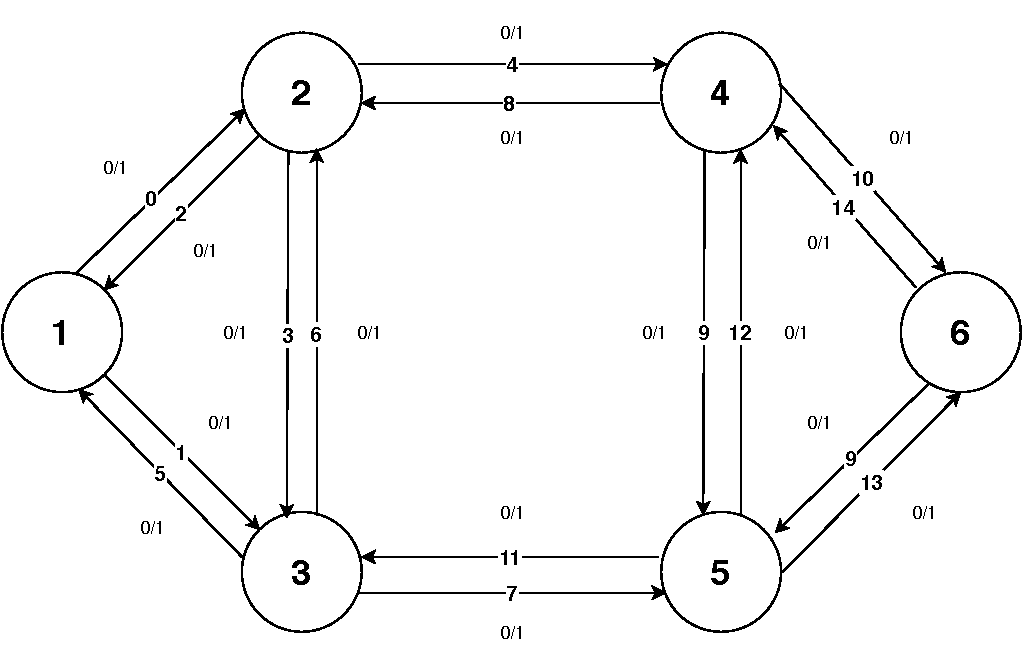
\includegraphics[width=12cm]{sdf/heuristic/transparent/figures/physicalTopology}
	\caption{Allowed physical topology.}
	\label{allowed_physical_surv_transp}
\end{figure}

\subsection{Logical topology matrix}
The network logical topology represents how the links and the nodes may interconnect with each other. In this particular case it is considered the transparent transport mode, and so each of the nodes will connect to others creating direct links between all nodes of the network. The same can be seen below represented in a matrix in table \ref{Transparentlogical_topology} and graphically in figure \ref{allowed_optical_surv_transparent2}.
\begin{table}[H]
	\centering	
	\begin{tabular}{|c|c|c|c|c|c|c|}
		\hline
		\multicolumn{1}{|l|}{\textbf{Nodes}} & 1   & 2   & 3   & 4   & 5   & 6  \\ \hline
		1                           & \textbf{0}   & 1 & 1 & 1 & 1 & 1 \\ \hline
		2                           & 1 & \textbf{0}   & 1 & 1 & 1 & 1 \\ \hline
		3                           & 1 & 1 & \textbf{0}   & 1 & 1 & 1 \\ \hline
		4                           & 1 & 1 & 1 & \textbf{0}   & 1 & 1 \\ \hline
		5                           & 1 & 1 & 1 & 1 & \textbf{0}   & 1 \\ \hline
		6                           & 1 & 1 & 1 & 1 & 1 & \textbf{0}   \\ \hline
	\end{tabular}
	\caption{Allowed logical topology matrix for transparent transport mode.}
	\label{Transparentlogical_topology}
\end{table}
\begin{figure}[H]
	\centering
	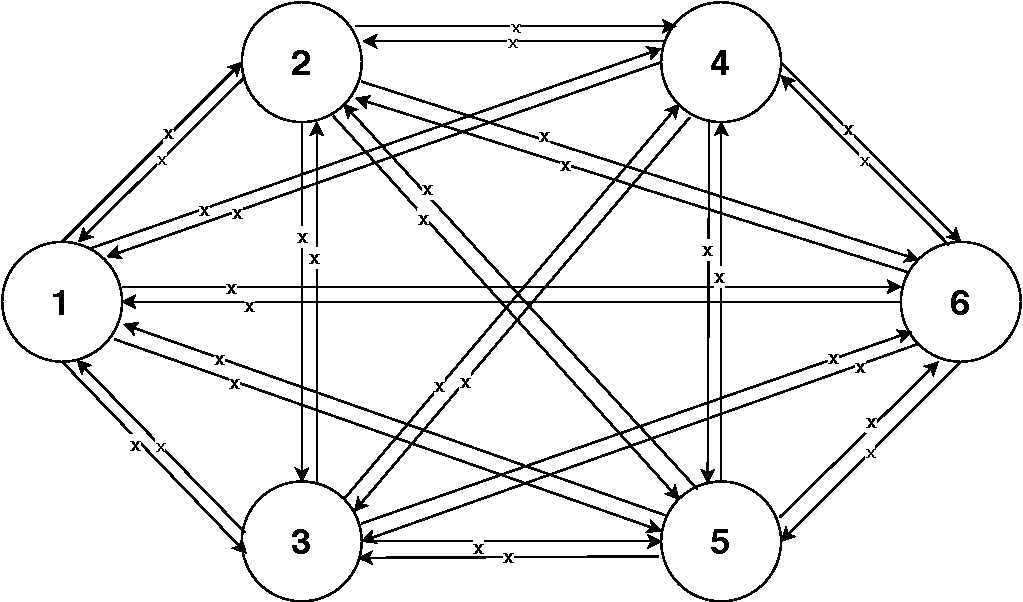
\includegraphics[width=10cm]{sdf/heuristic/transparent/figures/logicalTopology}
	\caption{Allowed logical topology graph.}
	\label{allowed_optical_surv_transparent2}
\end{figure}

\subsection{Traffic scenario}
The traffic matrices below are represented by ODU0, ODU1, ODU2, ODU3 and ODU4 where each one has a certain bit rate. The ODU0 corresponds to 1.25 Gbits/s, the ODU1 corresponds to 2.5 Gbits/s, the ODU2 corresponds to 10 Gbits/s, the ODU3 corresponds to 40 Gbits/s and finally the ODU4 corresponds to 100 Gbits/s.\\ \\
%As we can see below, these arrays are bi-directional because they are symmetric arrays and as such, the traffic sent in a certain direction must be the same traffic sent in that opposite direction.
Considering just 2 optical channels per opticalMultiplexingSystem, each with a capacity of 100 Gbps (80 ODU0s), and the following set of demands.\\ \\

\[
ODU0=
\begin{bmatrix}
0 & 0 & 0 & 0 & 0 & 0 \\
0 & 0 & 0 & 0 & 0 & 0 \\
0 & 0 & 0 & 0 & 0 & 0 \\
0 & 0 & 0 & 0 & 0 & 0 \\
0 & 0 & 0 & 0 & 0 & 0 \\
0 & 0 & 0 & 0 & 0 & 0
\end{bmatrix}
\qquad ODU1=
\begin{bmatrix}
0 & 0 & 0 & 0 & 0 & 0 \\
0 & 0 & 0 & 0 & 0 & 0 \\
0 & 0 & 0 & 0 & 0 & 0 \\
0 & 0 & 0 & 0 & 0 & 0 \\
0 & 0 & 0 & 0 & 0 & 0 \\
0 & 0 & 0 & 0 & 0 & 0
\end{bmatrix}
\]
\[
ODU2=
\begin{bmatrix}
0 & 0 & 0 & 0 & 0 & 0 \\
0 & 0 & 0 & 0 & 0 & 0 \\
0 & 0 & 0 & 0 & 0 & 0 \\
0 & 0 & 0 & 0 & 0 & 0 \\
0 & 0 & 0 & 0 & 0 & 0 \\
0 & 0 & 0 & 0 & 0 & 0
\end{bmatrix}
\qquad ODU3=
\begin{bmatrix}
0 & 0 & 0 & 0 & 0 & 0 \\
0 & 0 & 0 & 0 & 0 & 0 \\
0 & 0 & 0 & 0 & 2 & 0 \\
0 & 0 & 0 & 0 & 0 & 0 \\
0 & 0 & 0 & 0 & 0 & 0 \\
0 & 0 & 0 & 0 & 0 & 0
\end{bmatrix}
\]
\[
ODU4=
\begin{bmatrix}
0 & 0 & 0 & 0 & 5 & 0 \\
0 & 0 & 0 & 0 & 0 & 0 \\
0 & 0 & 0 & 0 & 0 & 0 \\
0 & 0 & 0 & 0 & 0 & 0 \\
0 & 0 & 0 & 0 & 0 & 0 \\
0 & 0 & 0 & 0 & 0 & 0
\end{bmatrix}
\]
\subsection{Theorectical resolution}
\vspace{17pt}
Through these ODU's we can calculate the total network traffic for this specific scenario:\\

$T_1^0$ = 0x1.25 = 0 Gbits/s \qquad
$T_1^1$ = 0x2.5 = 0 Gbits/s \qquad
$T_1^2$ = 0x10 = 0 Gbits/s \\

$T_1^3$ = 2x40 = 80 Gbits/s \quad
$T_1^4$ = 5x100 = 500 Gbits/s \\

$T_{1}$ = 0 + 0 + 0 + 80 + 500 = 580 Gbits/s \qquad \\
%$T$ = 1660/2 = \textbf{580 Gbits/s}\\

Where the variable $T_1^x$ represents the unidirectional traffic of the ODUx, for example, $T_1^0$ represents the unidirectional traffic of the ODU0 and $T_1^1$ represents the unidirectional traffic of the ODU1. The variable $T_{1}$ represents the total of unidirectional traffic that is injected into the network.\\

\textbf{Ordering demands}\\ \\
The demands are first ordered in the Scheduler\_   block considering the entry variable, orderingRule, in a single queue. It is assumed orderingRule to be equal to its default value descendingOrder, which will organize demand requests from ODU4 type demands to ODU0 type. These demands will constitute the Scheduler\_Out signal, which is a DemandRequest type signal.\\ 

\begin{table}[H]
	\centering
	\begin{tabular}{|c|c|c|c|c|}
		\hline
		demandIndex & sourceNode & destinationNode & oduType & survivabilityMethod \\ \hline
		0           & 1          & 5               & 4       & none                   \\ \hline
		1           & 1          & 5               & 4       & none                   \\ \hline
		2           & 1          & 5               & 4       & none                  \\ \hline
		3           & 1          & 5               & 4       & none                \\ \hline
		4           & 1          & 5               & 4       & none                \\ \hline
		5           & 3          & 5               & 3       & none                \\ \hline
		6           & 3          & 5               & 3       & none                \\ \hline
	\end{tabular}
	\caption{Demands ordered by Scheduler\_  block.}
	\label{scheduler_example}
\end{table}

\subsubsection{Demand 0}
\textbf{Generate a DemandRequest type signal}\\ \\
Demand 0 is sent in a DemandRequest type signal from the Scheduler\_  block to the LogicalTopologyManager\_  block.
\begin{table}[H]
	\centering
	\begin{tabular}{|c|c|c|c|c|}
		\hline
		demandIndex & sourceNode & destinationNode & oduType & survivabilityMethod \\ \hline
		0           & 1          & 5               & 4       & none                   \\ \hline
	\end{tabular}
	\caption{DemandRequest sent by Scheduler\_  block for demand 0.}
\end{table}
 
There, a search is made by an available path from source to destination node, in this case nodes 1 and 5, respectively.\\ \\

\textbf{Search for an availabe path}
\begin{table}[H]
	\centering
	\begin{tabular}{|c|c|c|c|c|}
		\hline
		pathIndex & sourceNode & destinationNode & \begin{tabular}[c]{@{}c@{}}capacity\\ (ODU0s)\end{tabular} & lightPathsIndex \\ \hline
		&            &                 &                                                            &                 \\ \hline
	\end{tabular}
	\caption{Paths state variable from LogicalTopologyManager\_  block.}
\end{table}
As initially no path exists, one must be created in order to route this demand and so a pathRequest type signal is sent from the LogicalTopologyManager\_  to to the PhysicalTopologyManager\_  block.\\ \\

\textbf{Apply Dijkstra algorithm to discover shortest logical paths}\\ \\

The logical topology matrix of table \ref{Transparentlogical_topology} is applied as an entry parameter to the Dijkstra algorithm. Considering the entry variables routingCriterionLogicalTopology as "Hops" (gives the shortest paths in terms of hops) and blockingCriterionLogicalTopology equal to 3, once in transparent transport mode only direct logical connections will concerne us, the output gives only the possibility of the direct logical connection (1->5) to establish a path between source and destination nodes, 1 and 5 respectively.\\ \\

\textbf{Generate a pathRequest signal}\\ \\

\begin{table}[H]
	\centering
	\begin{tabular}{|c|c|c|c|}
		\hline
		requestIndex & sourceNode & intermidiateNodes & destinationNode \\ \hline
		0            & 1          & -1                 & 5               \\ \hline
	\end{tabular}
	\caption{pathRequest signal for demand 0.}
\end{table} 

As the transport mode assumed is the transparent, only direct logical connections are used to route demands, and consequently there are no intermidiate nodes.\\ \\

\textbf{Apply Dijkstra algorithm to discover shortest physical paths}\\ \\
The physical topology matrix of table \ref{Adjacence_Matrix} is applied as an entry parameter to the Dijkstra algorithm. Here it is intended to convert the required light path (1->5) into a restricted variety of sets of physical connections, in this specific case 3. Considering blockingCriterionPhysicalTopology equal to 3 (number of paths to be tested before declaring a possible blocked state) and routingCriterionPhysicalTopology to be "Hops", then the final result of Dijkstra algorithm will be the one presented below.



\begin{table}[H]
	\centering
	\begin{tabular}{c|c|c|c|c|}
		\cline{2-5}
		& \multicolumn{4}{c|}{lightPath from nodes 1 to 5} \\ \cline{2-5} 
		& \multirow{2}{*}{sourceNode} & \multirow{2}{*}{destinationNode} & \multicolumn{2}{c|}{opticalChannels} \\ \cline{4-5} 
		&  &  & sourceNode & destinationNode \\ \cline{2-5} 
		\multirow{2}{*}{Shortest path 1} & \multirow{2}{*}{1} & \multirow{2}{*}{5} & 1 & 6 \\ \cline{4-5} 
		&  &  & 6 & 5 \\ \cline{2-5} 
		\multirow{3}{*}{Shortest path 2} & \multirow{3}{*}{1} & \multirow{3}{*}{5} & 1 & 2 \\ \cline{4-5} 
		&  &  & 2 & 3 \\ \cline{4-5} 
		&  &  & 3 & 5 \\ \cline{2-5} 
		\multirow{3}{*}{Shortest path 3} & \multirow{3}{*}{1} & \multirow{3}{*}{5} & 1 & 2 \\ \cline{4-5} 
		&  &  & 2 & 6 \\ \cline{4-5} 
		&  &  & 6 & 5 \\ \cline{2-5} 
	\end{tabular}
	\caption{Result of Dijkstra algorithm applied to the ajacence matrix.}
\end{table}

\textbf{Test shortest path 1}\\ 

\begin{table}[H]
	\centering
	\begin{tabular}{|c|c|c|c|c|c|}
		\hline
		\begin{tabular}[c]{@{}c@{}}opticalMultiplexing-\\ SystemIndex\end{tabular} & sourceNode & \begin{tabular}[c]{@{}c@{}}destination-\\ Node\end{tabular} & \begin{tabular}[c]{@{}c@{}}numberOf-\\ Wavelenghts\end{tabular} & \begin{tabular}[c]{@{}c@{}}wavelenghts\\ (nm)\end{tabular} & \begin{tabular}[c]{@{}c@{}}available-\\ Wavelenghts\end{tabular} \\ \hline
		1 & 1 & 6 & 2 & {[}1310 1550{]} & {[}1 1{]} \\ \hline
		15 & 6 & 5 & 2 & {[}1310 1550{]} & {[}1 1{]} \\ \hline
	\end{tabular}
	\caption{Initial values of opticalMultiplexingSystems going from node 1 to 6 and 6 to 5.}
\end{table}

As both opticalMultiplexingSystems have the required capacity and wavelenghts a PathRequestRouted signal will be generated informing the LogicalTopologyManager\_  block that it is possible to establish a path to route demand 0 through a lightPath using the opticalChannels above, and the physical capacity of the opticalMultiplexingSystems of the network will be updated.\\ 

\begin{table}[H]
	\centering
	\begin{tabular}{|c|c|c|c|c|c|}
		\hline
		\begin{tabular}[c]{@{}c@{}}opticalMultiplexing-\\ SystemIndex\end{tabular} & sourceNode & \begin{tabular}[c]{@{}c@{}}destination-\\ Node\end{tabular} & \begin{tabular}[c]{@{}c@{}}numberOf-\\ Wavelenghts\end{tabular} & \begin{tabular}[c]{@{}c@{}}wavelenghts\\ (nm)\end{tabular} & \begin{tabular}[c]{@{}c@{}}available-\\ Wavelenghts\end{tabular} \\ \hline
		1 & 1 & 6 & 2 & {[}1310 1550{]} & {[}0 1{]} \\ \hline
		15 & 6 & 5 & 2 & {[}1310 1550{]} & {[}0 1{]} \\ \hline
	\end{tabular}
	\caption{After values of opticalMultiplexingSystems going from node 1 to 6 and 6 to 5.}
\end{table}

In both Optical Multiplexing Systems an Optical Channel is going to be used in the creation of a Light Path in order to route demand 0. In this specific case the wavelenght used is 1310 nm which will remain unavailable for other demands that will not use this Light Path.\\ \\ 

\textbf{Generate a PathRequestRouted type signal}\\ 
\begin{table}[H]
	\centering
	\begin{tabular}{|c|c|c|}
		\hline
		requestIndex & routed & numberOfLightPaths \\ \hline
		0 & true & 1 \\ \hline
	\end{tabular}
	\caption{pathInformation variable from PathRequestRouted signal.}
\end{table}

\begin{table}[H]
	\centering
\begin{tabular}{|c|c|c|c|c|}
	\hline
	sourceNode & destinationNode & numberOfIntermediateNodes & intermediateNodes & \begin{tabular}[c]{@{}c@{}}wavelenght\\ (nm)\end{tabular} \\ \hline
	1 & 5 & 1 & {[}6{]} & 1310 \\ \hline
\end{tabular}
\caption{lightPathsTable variable from PathRequestRouted signal.}
\end{table}

\textbf{Update LogicalTopologyManager\_  block state variables} \\

\begin{table}[H]
	\centering
\begin{tabular}{|c|c|c|c|c|c|}
	\hline
	pathIndex & sourceNode & destinationNodes & \begin{tabular}[c]{@{}c@{}}capacity\\ (ODU0s)\end{tabular} & numberOfLightPaths & lightPathsIndex \\ \hline
	0 & 1 & 5 & 0 & 1 & 0 \\ \hline
\end{tabular}
	\caption{Paths variable updated.}
\end{table}

\begin{table}[H]
	\centering
\begin{tabular}{|c|c|c|c|c|c|}
	\hline
	lightPathIndex & sourceNode & destinationNode & \begin{tabular}[c]{@{}c@{}}capacity\\ (ODU0s)\end{tabular} & \begin{tabular}[c]{@{}c@{}}numberOfOptical-\\ Channels\end{tabular} & \begin{tabular}[c]{@{}c@{}}opticalChannles-\\ Index\end{tabular} \\ \hline
	0 & 1 & 5 & 0 & 2 & {[}0,1{]} \\ \hline
\end{tabular}
	\caption{LightPaths variable updated.}
\end{table}

\begin{table}[H]
	\centering
	\begin{tabular}{|c|c|c|c|c|c|c|}
		\hline
		\begin{tabular}[c]{@{}c@{}}opticalChannel-\\ Index\end{tabular} & sourceNode & \begin{tabular}[c]{@{}c@{}}destination-\\ Node\end{tabular} & \begin{tabular}[c]{@{}c@{}}capacity\\ (ODU0s)\end{tabular} & \begin{tabular}[c]{@{}c@{}}wavelenght\\ (nm)\end{tabular} & \begin{tabular}[c]{@{}c@{}}numberOf-\\ Demands\end{tabular} & \begin{tabular}[c]{@{}c@{}}demands-\\ Index\end{tabular} \\ \hline
		0 & 1 & 6 & 0 & 1310 & 1 & {[}0{]} \\ \hline
		1 & 6 & 5 & 0 & 1310 & 1 & {[}0{]} \\ \hline
	\end{tabular}
	\caption{OpticalChannels variable updated.}
\end{table}

\begin{table}[H]
	\centering	
	\begin{tabular}{|c|c|c|c|c|c|c|}
		\hline
		\multicolumn{1}{|l|}{\textbf{Nodes}} & 1   & 2   & 3   & 4   & 5   & 6  \\ \hline
		1                           & \textbf{0}   & 1 & 1 & 1 & 1 & 1 \\ \hline
		2                           & 1 & \textbf{0}   & 1 & 1 & 1 & 1 \\ \hline
		3                           & 1 & 1 & \textbf{0}   & 1 & 1 & 1 \\ \hline
		4                           & 1 & 1 & 1 & \textbf{0}   & 1 & 1 \\ \hline
		5                           & 1 & 1 & 1 & 1 & \textbf{0}   & 1 \\ \hline
		6                           & 1 & 1 & 1 & 1 & 1 & \textbf{0}   \\ \hline
	\end{tabular}
	\caption{logicalTopologyMatrix variable updated.}
	\label{Transparentlogical_topology_updated}
\end{table}

\textbf{Generate a DemandRequestRouted type signal}\\ \\

\begin{table}[H]
	\centering
\begin{tabular}{|c|c|c|}
	\hline
	demandIndex & routed & pathsIndex \\ \hline
	0 & true & 0 \\ \hline
\end{tabular}
	\caption{DemandRequestRouted signal.}
\end{table}

Finally this signal is sent to the last block of the diagram, SinkRoutedOrBlocked\_.
\subsection{Demand 1}
\textbf{Generate a DemandRequest type signal}\\ \\
Demand 1 is sent in a DemandRequest type signal from the Scheduler\_  block to the LogicalTopologyManager\_  block.
\begin{table}[H]
	\centering
	\begin{tabular}{|c|c|c|c|c|}
		\hline
		demandIndex & sourceNode & destinationNode & oduType & survivabilityMethod \\ \hline
		1           & 1          & 5               & 4       & none                   \\ \hline
	\end{tabular}
	\caption{DemandRequest sent by Scheduler\_  block for demand 1.}
\end{table}

There, a search is made by an available path from source to destination node, in this case nodes 1 and 5, respectively.\\ \\

\textbf{Search for an availabe path}
\begin{table}[H]
	\centering
	\begin{tabular}{|c|c|c|c|c|c|}
		\hline
		pathIndex & sourceNode & destinationNodes & \begin{tabular}[c]{@{}c@{}}capacity\\ (ODU0s)\end{tabular} & numberOfLightPaths & lightPathsIndex \\ \hline
		0 & 1 & 5 & 0 & 1 & 0 \\ \hline
	\end{tabular}
	\caption{Paths state variable from LogicalTopologyManager\_  block.}
\end{table}
As there is no path available with remaning capacity to route an ODU4 demand, one must be created in order to route this demand 1 and so a pathRequest type signal is sent from the LogicalTopologyManager\_  to to the PhysicalTopologyManager\_  block.\\ \\

\textbf{Apply Dijkstra algorithm to discover shortest logical paths}\\ \\

The logical topology matrix of table \ref{Transparentlogical_topology_updated} is applied as an entry parameter to the Dijkstra algorithm. Considering the entry variables routingCriterionLogicalTopology as "Hops" (gives the shortest paths in terms of hops) and blockingCriterionLogicalTopology equal to 3, once in transparent transport mode only direct logical connections will concerne us, the output gives only the possibility of the direct logical connection (1->5) to establish a path between source and destination nodes, 1 and 5 respectively.\\ \\

\textbf{Generate a pathRequest signal}\\ \\

\begin{table}[H]
	\centering
	\begin{tabular}{|c|c|c|c|}
		\hline
		requestIndex & sourceNode & intermidiateNodes & destinationNode \\ \hline
		1            & 1          & -1                 & 5               \\ \hline
	\end{tabular}
	\caption{pathRequest signal for demand 0.}
\end{table} 

As the transport mode assumed is the transparent, only direct logical connections are used to route demands, and consequently there are no intermidiate nodes.\\ \\

\textbf{Apply Dijkstra algorithm to discover shortest physical paths}\\ \\
The physical topology matrix of table \ref{Adjacence_Matrix} is applied as an entry parameter to the Dijkstra algorithm. Here it is intended to convert the required light path (1->5) into a restricted variety of sets of physical connections, in this specific case 3. Considering blockingCriterionPhysicalTopology equal to 3 (number of paths to be tested before declaring a possible blocked state) and routingCriterionPhysicalTopology to be "Hops", then the final result of Dijkstra algorithm will be the one presented below.



\begin{table}[H]
	\centering
	\begin{tabular}{c|c|c|c|c|}
		\cline{2-5}
		& \multicolumn{4}{c|}{lightPath from nodes 1 to 5} \\ \cline{2-5} 
		& \multirow{2}{*}{sourceNode} & \multirow{2}{*}{destinationNode} & \multicolumn{2}{c|}{opticalChannels} \\ \cline{4-5} 
		&  &  & sourceNode & destinationNode \\ \cline{2-5} 
		\multirow{2}{*}{Shortest path 1} & \multirow{2}{*}{1} & \multirow{2}{*}{5} & 1 & 6 \\ \cline{4-5} 
		&  &  & 6 & 5 \\ \cline{2-5} 
		\multirow{3}{*}{Shortest path 2} & \multirow{3}{*}{1} & \multirow{3}{*}{5} & 1 & 2 \\ \cline{4-5} 
		&  &  & 2 & 3 \\ \cline{4-5} 
		&  &  & 3 & 5 \\ \cline{2-5} 
		\multirow{3}{*}{Shortest path 3} & \multirow{3}{*}{1} & \multirow{3}{*}{5} & 1 & 2 \\ \cline{4-5} 
		&  &  & 2 & 6 \\ \cline{4-5} 
		&  &  & 6 & 5 \\ \cline{2-5} 
	\end{tabular}
	\caption{Result of Dijkstra algorithm applied to the ajacence matrix.}
\end{table}

\textbf{Test shortest path 1}\\ 

\begin{table}[H]
	\centering
	\begin{tabular}{|c|c|c|c|c|c|}
		\hline
		\begin{tabular}[c]{@{}c@{}}opticalMultiplexing-\\ SystemIndex\end{tabular} & sourceNode & \begin{tabular}[c]{@{}c@{}}destination-\\ Node\end{tabular} & \begin{tabular}[c]{@{}c@{}}numberOf-\\ Wavelenghts\end{tabular} & \begin{tabular}[c]{@{}c@{}}wavelenghts\\ (nm)\end{tabular} & \begin{tabular}[c]{@{}c@{}}available-\\ Wavelenghts\end{tabular} \\ \hline
		1 & 1 & 6 & 2 & {[}1310 1550{]} & {[}0 1{]} \\ \hline
		15 & 6 & 5 & 2 & {[}1310 1550{]} & {[}0 1{]} \\ \hline
	\end{tabular}
	\caption{Initial values of opticalMultiplexingSystems going from node 1 to 6 and 6 to 5.}
\end{table}

As both opticalMultiplexingSystems have the required capacity and wavelenghts a PathRequestRouted signal will be generated informing the LogicalTopologyManager\_  block that it is possible to establish a path to route demand 1 through a lightPath using the opticalChannels above, and the physical capacity of the opticalMultiplexingSystems of the network will be updated.\\ 

\begin{table}[H]
	\centering
	\begin{tabular}{|c|c|c|c|c|c|}
		\hline
		\begin{tabular}[c]{@{}c@{}}opticalMultiplexing-\\ SystemIndex\end{tabular} & sourceNode & \begin{tabular}[c]{@{}c@{}}destination-\\ Node\end{tabular} & \begin{tabular}[c]{@{}c@{}}numberOf-\\ Wavelenghts\end{tabular} & \begin{tabular}[c]{@{}c@{}}wavelenghts\\ (nm)\end{tabular} & \begin{tabular}[c]{@{}c@{}}available-\\ Wavelenghts\end{tabular} \\ \hline
		1 & 1 & 6 & 2 & {[}1310 1550{]} & {[}0 0{]} \\ \hline
		15 & 6 & 5 & 2 & {[}1310 1550{]} & {[}0 0{]} \\ \hline
	\end{tabular}
	\caption{After values of opticalMultiplexingSystems going from node 1 to 6 and 6 to 5.}
\end{table}

In both Optical Multiplexing Systems an Optical Channel is going to be used in the creation of a Light Path in order to route demand 1. In this specific case the wavelenght used is 1550 nm which will remain unavailable for other demands that will not use this Light Path.\\


\textbf{Generate a PathRequestRouted type signal}\\ 
\begin{table}[H]
	\centering
	\begin{tabular}{|c|c|c|}
		\hline
		requestIndex & routed & numberOfLightPaths \\ \hline
		1 & true & 1 \\ \hline
	\end{tabular}
	\caption{pathInformation variable from PathRequestRouted signal.}
\end{table}

\begin{table}[H]
	\centering
	\begin{tabular}{|c|c|c|c|c|}
		\hline
		sourceNode & destinationNode & numberOfIntermediateNodes & intermediateNodes & \begin{tabular}[c]{@{}c@{}}wavelenght\\ (nm)\end{tabular} \\ \hline
		1 & 5 & 1 & {[}6{]} & 1550 \\ \hline
	\end{tabular}
	\caption{lightPathsTable variable from PathRequestRouted signal.}
\end{table}

\textbf{Update LogicalTopologyManager\_  block state variables} \\

\begin{table}[H]
	\centering
	\begin{tabular}{|c|c|c|c|c|c|}
		\hline
		pathIndex & sourceNode & destinationNodes & \begin{tabular}[c]{@{}c@{}}capacity\\ (ODU0s)\end{tabular} & numberOfLightPaths & lightPathsIndex \\ \hline
		0 & 1 & 5 & 0 & 1 & 0 \\ \hline
		1 & 1 & 5 & 0 & 1 & 1 \\ \hline
	\end{tabular}
	\caption{Paths variable updated.}
\end{table}

\begin{table}[H]
	\centering
	\begin{tabular}{|c|c|c|c|c|c|}
		\hline
		lightPathIndex & sourceNode & destinationNode & \begin{tabular}[c]{@{}c@{}}capacity\\ (ODU0s)\end{tabular} & \begin{tabular}[c]{@{}c@{}}numberOfOptical-\\ Channels\end{tabular} & \begin{tabular}[c]{@{}c@{}}opticalChannles-\\ Index\end{tabular} \\ \hline
		0 & 1 & 5 & 0 & 2 & {[}0,1{]} \\ \hline
		1 & 1 & 5 & 0 & 2 & {[}2,3{]} \\ \hline
	\end{tabular}
	\caption{LightPaths variable updated.}
\end{table}

\begin{table}[H]
	\centering
	\begin{tabular}{|c|c|c|c|c|c|c|}
		\hline
		\begin{tabular}[c]{@{}c@{}}opticalChannel-\\ Index\end{tabular} & sourceNode & \begin{tabular}[c]{@{}c@{}}destination-\\ Node\end{tabular} & \begin{tabular}[c]{@{}c@{}}capacity\\ (ODU0s)\end{tabular} & \begin{tabular}[c]{@{}c@{}}wavelenght\\ (nm)\end{tabular} & \begin{tabular}[c]{@{}c@{}}numberOf-\\ Demands\end{tabular} & \begin{tabular}[c]{@{}c@{}}demands-\\ Index\end{tabular} \\ \hline
		0 & 1 & 6 & 0 & 1310 & 1 & {[}0{]} \\ \hline
		1 & 6 & 5 & 0 & 1310 & 1 & {[}0{]} \\ \hline
		2 & 1 & 6 & 0 & 1550 & 1 & {[}1{]} \\ \hline
		3 & 6 & 5 & 0 & 1550 & 1 & {[}1{]} \\ \hline
	\end{tabular}
	\caption{OpticalChannels variable updated.}
\end{table}

\begin{table}[H]
	\centering	
	\begin{tabular}{|c|c|c|c|c|c|c|}
		\hline
		\multicolumn{1}{|l|}{\textbf{Nodes}} & 1   & 2   & 3   & 4   & 5   & 6  \\ \hline
		1                           & \textbf{0}   & 1 & 1 & 1 & 1 & 1 \\ \hline
		2                           & 1 & \textbf{0}   & 1 & 1 & 1 & 1 \\ \hline
		3                           & 1 & 1 & \textbf{0}   & 1 & 1 & 1 \\ \hline
		4                           & 1 & 1 & 1 & \textbf{0}   & 1 & 1 \\ \hline
		5                           & 1 & 1 & 1 & 1 & \textbf{0}   & 1 \\ \hline
		6                           & 1 & 1 & 1 & 1 & 1 & \textbf{0}   \\ \hline
	\end{tabular}
	\caption{logicalTopologyMatrix variable updated.}
	\label{Transparentlogical_topology_updated}
\end{table}

\textbf{Generate a DemandRequestRouted type signal}\\ \\

\begin{table}[H]
	\centering
	\begin{tabular}{|c|c|c|}
		\hline
		demandIndex & routed & pathsIndex \\ \hline
		1 & true & 1 \\ \hline
	\end{tabular}
	\caption{DemandRequestRouted signal.}
\end{table}

Finally this signal is sent to the last block of the diagram, SinkRoutedOrBlocked\_.
\subsection{Demand 2}
\textbf{Generate a DemandRequest type signal}\\ \\
Demand 2 is sent in a DemandRequest type signal from the Scheduler\_  block to the LogicalTopologyManager\_  block.
\begin{table}[H]
	\centering
	\begin{tabular}{|c|c|c|c|c|}
		\hline
		demandIndex & sourceNode & destinationNode & oduType & survivabilityMethod \\ \hline
		2           & 1          & 5               & 4       & none                   \\ \hline
	\end{tabular}
	\caption{DemandRequest sent by Scheduler\_  block for demand 2.}
\end{table}

There, a search is made by an available path from source to destination node, in this case nodes 1 and 5, respectively.\\ \\

\textbf{Search for an availabe path}
\begin{table}[H]
	\centering
	\begin{tabular}{|c|c|c|c|c|c|}
		\hline
		pathIndex & sourceNode & destinationNodes & \begin{tabular}[c]{@{}c@{}}capacity\\ (ODU0s)\end{tabular} & numberOfLightPaths & lightPathsIndex \\ \hline
		0 & 1 & 5 & 0 & 1 & 0 \\ \hline
		1 & 1 & 5 & 0 & 1 & 1 \\ \hline
	\end{tabular}
	\caption{Paths state variable from LogicalTopologyManager\_  block.}
\end{table}
As there is no path available with remaning capacity to route an ODU4 demand, one must be created in order to route this demand 2 and so a pathRequest type signal is sent from the LogicalTopologyManager\_  to to the PhysicalTopologyManager\_  block.\\ \\

\textbf{Apply Dijkstra algorithm to discover shortest logical paths}\\ \\

The logical topology matrix of table \ref{Transparentlogical_topology_updated} is applied as an entry parameter to the Dijkstra algorithm. Considering the entry variables routingCriterionLogicalTopology as "Hops" (gives the shortest paths in terms of hops) and blockingCriterionLogicalTopology equal to 3, once in transparent transport mode only direct logical connections will concerne us, the output gives only the possibility of the direct logical connection (1->5) to establish a path between source and destination nodes, 1 and 5 respectively.\\ \\

\textbf{Generate a pathRequest signal}\\ \\

\begin{table}[H]
	\centering
	\begin{tabular}{|c|c|c|c|}
		\hline
		requestIndex & sourceNode & intermidiateNodes & destinationNode \\ \hline
		2            & 1          & -1                 & 5               \\ \hline
	\end{tabular}  
	\caption{pathRequest signal for demand 0.}
\end{table} 

As the transport mode assumed is the transparent, only direct logical connections are used to route demands, and consequently there are no intermidiate nodes.\\ \\

\textbf{Apply Dijkstra algorithm to discover shortest physical paths}\\ \\
The physical topology matrix of table \ref{Adjacence_Matrix} is applied as an entry parameter to the Dijkstra algorithm. Here it is intended to convert the required light path (1->5) into a restricted variety of sets of physical connections, in this specific case 3. Considering blockingCriterionPhysicalTopology equal to 3 (number of paths to be tested before declaring a possible blocked state) and routingCriterionPhysicalTopology to be "Hops", then the final result of Dijkstra algorithm will be the one presented below.



\begin{table}[H]
	\centering
	\begin{tabular}{c|c|c|c|c|}
		\cline{2-5}
		& \multicolumn{4}{c|}{lightPath from nodes 1 to 5} \\ \cline{2-5} 
		& \multirow{2}{*}{sourceNode} & \multirow{2}{*}{destinationNode} & \multicolumn{2}{c|}{opticalChannels} \\ \cline{4-5} 
		&  &  & sourceNode & destinationNode \\ \cline{2-5} 
		\multirow{2}{*}{Shortest path 1} & \multirow{2}{*}{1} & \multirow{2}{*}{5} & 1 & 6 \\ \cline{4-5} 
		&  &  & 6 & 5 \\ \cline{2-5} 
		\multirow{3}{*}{Shortest path 2} & \multirow{3}{*}{1} & \multirow{3}{*}{5} & 1 & 2 \\ \cline{4-5} 
		&  &  & 2 & 3 \\ \cline{4-5} 
		&  &  & 3 & 5 \\ \cline{2-5} 
		\multirow{3}{*}{Shortest path 3} & \multirow{3}{*}{1} & \multirow{3}{*}{5} & 1 & 2 \\ \cline{4-5} 
		&  &  & 2 & 6 \\ \cline{4-5} 
		&  &  & 6 & 5 \\ \cline{2-5} 
	\end{tabular}
	\caption{Result of Dijkstra algorithm applied to the ajacence matrix.}
\end{table}

\textbf{Test shortest path 1}\\ 

\begin{table}[H]
	\centering
	\begin{tabular}{|c|c|c|c|c|c|}
		\hline
		\begin{tabular}[c]{@{}c@{}}opticalMultiplexing-\\ SystemIndex\end{tabular} & sourceNode & \begin{tabular}[c]{@{}c@{}}destination-\\ Node\end{tabular} & \begin{tabular}[c]{@{}c@{}}numberOf-\\ Wavelenghts\end{tabular} & \begin{tabular}[c]{@{}c@{}}wavelenghts\\ (nm)\end{tabular} & \begin{tabular}[c]{@{}c@{}}available-\\ Wavelenghts\end{tabular} \\ \hline
		1 & 1 & 6 & 2 & {[}1310 1550{]} & {[}0 0{]} \\ \hline
		15 & 6 & 5 & 2 & {[}1310 1550{]} & {[}0 0{]} \\ \hline
	\end{tabular}
	\caption{Initial values of opticalMultiplexingSystems going from node 1 to 6 and 6 to 5.}
\end{table}

As both opticalMultiplexingSystems are already completely full then they will remain unavailable for demands to use and so the physical topology must be updated so that Dijkstra algorithm does not take into account this Optical Multiplexing Systems for shortest path creating processes in further iterations.\\ \\

\textbf{Update physical topology matrix}\\ 
\begin{table}[H]
	\centering
	\begin{tabular}{|c|c|c|c|c|c|c|}
		\hline
		\textbf{Nodes} & 1 & 2 & 3 & 4 & 5 & 6 \\ \hline
		1     & \textbf{0} & 1 & 0 & 0 & 0 & 0 \\ \hline
		2     & 1 & \textbf{0} & 1 & 0 & 0 & 1 \\ \hline
		3     & 0 & 1 & \textbf{0} & 1 & 1 & 0 \\ \hline
		4     & 0 & 0 & 1 & \textbf{0} & 1 & 0 \\ \hline
		5     & 0 & 0 & 1 & 1 & \textbf{0} & 1 \\ \hline
		6     & 1 & 1 & 0 & 0 & 0 & \textbf{0} \\ \hline
	\end{tabular}
	\caption{Updated physical topology matrix.}
	\label{Adjacence_Matrix}
\end{table}


\textbf{Test shortest path 2}\\ 
\begin{table}[H]
	\centering
\begin{tabular}{|c|c|c|c|c|c|}
	\hline
	\begin{tabular}[c]{@{}c@{}}opticalMultiplexing-\\ SystemIndex\end{tabular} & sourceNode & \begin{tabular}[c]{@{}c@{}}destination-\\ Node\end{tabular} & \begin{tabular}[c]{@{}c@{}}numberOf-\\ Wavelenghts\end{tabular} & \begin{tabular}[c]{@{}c@{}}wavelenghts\\ (nm)\end{tabular} & \begin{tabular}[c]{@{}c@{}}available-\\ Wavelenghts\end{tabular} \\ \hline
	0 & 1 & 2 & 2 & {[}1310 1550{]} & {[}1 1{]} \\ \hline
	3 & 2 & 3 & 2 & {[}1310 1550{]} & {[}1 1{]} \\ \hline
	7 & 3 & 5 & 2 & {[}1310 1550{]} & {[}1 1{]} \\ \hline
\end{tabular}
	\caption{Initial values of opticalMultiplexingSystems going from nodes 1 to 2, 2 to 3 and 3 to 5.}
\end{table}

\begin{table}[H]
	\centering
\begin{tabular}{|c|c|c|c|c|c|}
	\hline
	\begin{tabular}[c]{@{}c@{}}opticalMultiplexing-\\ SystemIndex\end{tabular} & sourceNode & \begin{tabular}[c]{@{}c@{}}destination-\\ Node\end{tabular} & \begin{tabular}[c]{@{}c@{}}numberOf-\\ Wavelenghts\end{tabular} & \begin{tabular}[c]{@{}c@{}}wavelenghts\\ (nm)\end{tabular} & \begin{tabular}[c]{@{}c@{}}available-\\ Wavelenghts\end{tabular} \\ \hline
	0 & 1 & 2 & 2 & {[}1310 1550{]} & {[}0 1{]} \\ \hline
	3 & 2 & 3 & 2 & {[}1310 1550{]} & {[}0 1{]} \\ \hline
	7 & 3 & 5 & 2 & {[}1310 1550{]} & {[}0 1{]} \\ \hline
\end{tabular}
	\caption{After values of opticalMultiplexingSystems going from nodes 1 to 2, 2 to 3 and 3 to 5.}
\end{table}

In both Optical Multiplexing Systems an Optical Channel is going to be used in the creation of a Light Path in order to route demand 2. In this specific case the wavelenght used is 1310 nm which will remain unavailable for other demands that will not use this Light Path.\\


\textbf{Generate a PathRequestRouted type signal}\\ 
\begin{table}[H]
	\centering
	\begin{tabular}{|c|c|c|}
		\hline
		requestIndex & routed & numberOfLightPaths \\ \hline
		2 & true & 1 \\ \hline
	\end{tabular}
	\caption{pathInformation variable from PathRequestRouted signal.}
\end{table}

\begin{table}[H]
	\centering
	\begin{tabular}{|c|c|c|c|c|}
		\hline
		sourceNode & destinationNode & numberOfIntermediateNodes & intermediateNodes & \begin{tabular}[c]{@{}c@{}}wavelenght\\ (nm)\end{tabular} \\ \hline
		1 & 5 & 2 & {[}2 3{]} & 1310 \\ \hline
	\end{tabular}
	\caption{lightPathsTable variable from PathRequestRouted signal.}
\end{table}

\textbf{Update LogicalTopologyManager\_  block state variables} \\

\begin{table}[H]
	\centering
	\begin{tabular}{|c|c|c|c|c|c|}
		\hline
		pathIndex & sourceNode & destinationNodes & \begin{tabular}[c]{@{}c@{}}capacity\\ (ODU0s)\end{tabular} & numberOfLightPaths & lightPathsIndex \\ \hline
		0 & 1 & 5 & 0 & 1 & 0 \\ \hline
		1 & 1 & 5 & 0 & 1 & 1 \\ \hline
		2 & 1 & 5 & 0 & 1 & 2 \\ \hline
	\end{tabular}
	\caption{Paths variable updated.}
\end{table}

\begin{table}[H]
	\centering
	\begin{tabular}{|c|c|c|c|c|c|}
		\hline
		lightPathIndex & sourceNode & destinationNode & \begin{tabular}[c]{@{}c@{}}capacity\\ (ODU0s)\end{tabular} & \begin{tabular}[c]{@{}c@{}}numberOfOptical-\\ Channels\end{tabular} & \begin{tabular}[c]{@{}c@{}}opticalChannles-\\ Index\end{tabular} \\ \hline
		0 & 1 & 5 & 0 & 2 & {[}0,1{]} \\ \hline
		1 & 1 & 5 & 0 & 2 & {[}2,3{]} \\ \hline
		2 & 1 & 5 & 0 & 3 & {[}4,5,6{]} \\ \hline
	\end{tabular}
	\caption{LightPaths variable updated.}
\end{table}

\begin{table}[H]
	\centering
	\begin{tabular}{|c|c|c|c|c|c|c|}
		\hline
		\begin{tabular}[c]{@{}c@{}}opticalChannel-\\ Index\end{tabular} & sourceNode & \begin{tabular}[c]{@{}c@{}}destination-\\ Node\end{tabular} & \begin{tabular}[c]{@{}c@{}}capacity\\ (ODU0s)\end{tabular} & \begin{tabular}[c]{@{}c@{}}wavelenght\\ (nm)\end{tabular} & \begin{tabular}[c]{@{}c@{}}numberOf-\\ Demands\end{tabular} & \begin{tabular}[c]{@{}c@{}}demands-\\ Index\end{tabular} \\ \hline
		0 & 1 & 6 & 0 & 1310 & 1 & {[}0{]} \\ \hline
		1 & 6 & 5 & 0 & 1310 & 1 & {[}0{]} \\ \hline
		2 & 1 & 6 & 0 & 1550 & 1 & {[}1{]} \\ \hline
		3 & 6 & 5 & 0 & 1550 & 1 & {[}1{]} \\ \hline
		4 & 1 & 2 & 0 & 1310 & 1 & {[}2{]} \\ \hline
		5 & 2 & 3 & 0 & 1310 & 1 & {[}2{]} \\ \hline
		6 & 3 & 5 & 0 & 1310 & 1 & {[}2{]} \\ \hline
	\end{tabular}
	\caption{OpticalChannels variable updated.}
\end{table}

\begin{table}[H]
	\centering	
	\begin{tabular}{|c|c|c|c|c|c|c|}
		\hline
		\multicolumn{1}{|l|}{\textbf{Nodes}} & 1   & 2   & 3   & 4   & 5   & 6  \\ \hline
		1                           & \textbf{0}   & 1 & 1 & 1 & 1 & 1 \\ \hline
		2                           & 1 & \textbf{0}   & 1 & 1 & 1 & 1 \\ \hline
		3                           & 1 & 1 & \textbf{0}   & 1 & 1 & 1 \\ \hline
		4                           & 1 & 1 & 1 & \textbf{0}   & 1 & 1 \\ \hline
		5                           & 1 & 1 & 1 & 1 & \textbf{0}   & 1 \\ \hline
		6                           & 1 & 1 & 1 & 1 & 1 & \textbf{0}   \\ \hline
	\end{tabular}
	\caption{logicalTopologyMatrix variable updated.}
	\label{Transparentlogical_topology_updated}
\end{table}

\textbf{Generate a DemandRequestRouted type signal}\\ \\

\begin{table}[H]
	\centering
	\begin{tabular}{|c|c|c|}
		\hline
		demandIndex & routed & pathsIndex \\ \hline
		2 & true & 2 \\ \hline
	\end{tabular}
	\caption{DemandRequestRouted signal.}
\end{table}

Finally this signal is sent to the last block of the diagram, SinkRoutedOrBlocked\_.
\subsection{Demand 3}
\textbf{Generate a DemandRequest type signal}\\ \\
Demand 3 is sent in a DemandRequest type signal from the Scheduler\_  block to the LogicalTopologyManager\_  block.
\begin{table}[H]
	\centering
	\begin{tabular}{|c|c|c|c|c|}
		\hline
		demandIndex & sourceNode & destinationNode & oduType & survivabilityMethod \\ \hline
		3           & 1          & 5               & 4       & none                   \\ \hline
	\end{tabular}
	\caption{DemandRequest sent by Scheduler\_  block for demand 3.}
\end{table}

There, a search is made by an available path from source to destination node, in this case nodes 1 and 5, respectively.\\ \\

\textbf{Search for an availabe path}
\begin{table}[H]
	\centering
	\begin{tabular}{|c|c|c|c|c|c|}
		\hline
		pathIndex & sourceNode & destinationNodes & \begin{tabular}[c]{@{}c@{}}capacity\\ (ODU0s)\end{tabular} & numberOfLightPaths & lightPathsIndex \\ \hline
		0 & 1 & 5 & 0 & 1 & 0 \\ \hline
		1 & 1 & 5 & 0 & 1 & 1 \\ \hline
		2 & 1 & 5 & 0 & 1 & 2 \\ \hline
	\end{tabular}
	\caption{Paths state variable from LogicalTopologyManager\_  block.}
\end{table}
As there is no path available with remaning capacity to route an ODU4 demand, one must be created in order to route this demand 1 and so a pathRequest type signal is sent from the LogicalTopologyManager\_  to to the PhysicalTopologyManager\_  block.\\ \\

\textbf{Apply Dijkstra algorithm to discover shortest logical paths}\\ \\

The logical topology matrix of table \ref{Transparentlogical_topology_updated} is applied as an entry parameter to the Dijkstra algorithm. Considering the entry variables routingCriterionLogicalTopology as "Hops" (gives the shortest paths in terms of hops) and blockingCriterionLogicalTopology equal to 3, once in transparent transport mode only direct logical connections will concerne us, the output gives only the possibility of the direct logical connection (1->5) to establish a path between source and destination nodes, 1 and 5 respectively.\\ \\

\textbf{Generate a pathRequest signal}\\ \\

\begin{table}[H]
	\centering
	\begin{tabular}{|c|c|c|c|}
		\hline
		requestIndex & sourceNode & intermidiateNodes & destinationNode \\ \hline
		3            & 1          & -1                 & 5               \\ \hline
	\end{tabular}
	\caption{pathRequest signal for demand 0.}
\end{table} 

As the transport mode assumed is the transparent, only direct logical connections are used to route demands, and consequently there are no intermidiate nodes.\\ \\

\textbf{Apply Dijkstra algorithm to discover shortest physical paths}\\ \\
The physical topology matrix already updated before of table xxx is applied as an entry parameter to the Dijkstra algorithm. Here it is intended to convert the required light path (1->5) into a restricted variety of sets of physical connections, in this specific case 3. Considering blockingCriterionPhysicalTopology equal to 3 (number of paths to be tested before declaring a possible blocked state) and routingCriterionPhysicalTopology to be "Hops", then the final result of Dijkstra algorithm will be the one presented below. Notice that once our entry physical topology is now different then the final output of Dijkstra algorithm will also differ.



\begin{table}[H]
	\centering
	\begin{tabular}{c|c|c|c|c|}
		\cline{2-5}
		& \multicolumn{4}{c|}{lightPath from nodes 1 to 5} \\ \cline{2-5} 
		& \multirow{2}{*}{sourceNode} & \multirow{2}{*}{destinationNode} & \multicolumn{2}{c|}{opticalChannels} \\ \cline{4-5} 
		&  &  & sourceNode & destinationNode \\ \cline{2-5} 
		\multirow{3}{*}{Shortest path 1} & \multirow{3}{*}{1} & \multirow{3}{*}{5} & 1 & 2 \\ \cline{4-5} 
		&  &  & 2 & 3 \\ \cline{4-5} 
		&  &  & 3 & 5 \\ \cline{2-5} 
		\multirow{3}{*}{Shortest path 2} & \multirow{3}{*}{1} & \multirow{3}{*}{5} & 1 & 2 \\ \cline{4-5} 
		&  &  & 2 & 6 \\ \cline{4-5} 
		&  &  & 6 & 5 \\ \cline{2-5} 
		\multirow{4}{*}{Shortest path 3} & \multirow{4}{*}{1} & \multirow{4}{*}{5} & 1 & 2 \\ \cline{4-5} 
		&  &  & 2 & 3 \\ \cline{4-5} 
		&  &  & 3 & 4 \\ \cline{4-5} 
		&  &  & 4 & 5 \\ \cline{2-5} 
	\end{tabular}
	\caption{Result of Dijkstra algorithm applied to the ajacence matrix.}
\end{table}

\textbf{Test shortest path 1}\\ 

\begin{table}[H]
	\centering
\begin{tabular}{|c|c|c|c|c|c|}
	\hline
	\begin{tabular}[c]{@{}c@{}}opticalMultiplexing-\\ SystemIndex\end{tabular} & sourceNode & \begin{tabular}[c]{@{}c@{}}destination-\\ Node\end{tabular} & \begin{tabular}[c]{@{}c@{}}numberOf-\\ Wavelenghts\end{tabular} & \begin{tabular}[c]{@{}c@{}}wavelenghts\\ (nm)\end{tabular} & \begin{tabular}[c]{@{}c@{}}available-\\ Wavelenghts\end{tabular} \\ \hline
	0 & 1 & 2 & 2 & {[}1310 1550{]} & {[}0 1{]} \\ \hline
	3 & 2 & 3 & 2 & {[}1310 1550{]} & {[}0 1{]} \\ \hline
	7 & 3 & 5 & 2 & {[}1310 1550{]} & {[}0 1{]} \\ \hline
\end{tabular}
	\caption{Initial values of opticalMultiplexingSystems going from node 1 to 2, 2 to 3 and 3 to 5.}
\end{table}

As both opticalMultiplexingSystems have the required capacity and wavelenghts a PathRequestRouted signal will be generated informing the LogicalTopologyManager\_  block that it is possible to establish a path to route demand 1 through a lightPath using the opticalChannels above, and the physical capacity of the opticalMultiplexingSystems of the network will be updated.\\ 

\begin{table}[H]
	\centering
\begin{tabular}{|c|c|c|c|c|c|}
	\hline
	\begin{tabular}[c]{@{}c@{}}opticalMultiplexing-\\ SystemIndex\end{tabular} & sourceNode & \begin{tabular}[c]{@{}c@{}}destination-\\ Node\end{tabular} & \begin{tabular}[c]{@{}c@{}}numberOf-\\ Wavelenghts\end{tabular} & \begin{tabular}[c]{@{}c@{}}wavelenghts\\ (nm)\end{tabular} & \begin{tabular}[c]{@{}c@{}}available-\\ Wavelenghts\end{tabular} \\ \hline
	0 & 1 & 2 & 2 & {[}1310 1550{]} & {[}0 0{]} \\ \hline
	3 & 2 & 3 & 2 & {[}1310 1550{]} & {[}0 0{]} \\ \hline
	7 & 3 & 5 & 2 & {[}1310 1550{]} & {[}0 0{]} \\ \hline
\end{tabular}
	\caption{After values of opticalMultiplexingSystems going from node 1 to 2, 2 to 3 and 3 to 5.}
\end{table}

In both Optical Multiplexing Systems an Optical Channel is going to be used in the creation of a Light Path in order to route demand 3. In this specific case the wavelenght used is 1550 nm which will remain unavailable for other demands that will not use this Light Path.\\


\textbf{Generate a PathRequestRouted type signal}\\ 
\begin{table}[H]
	\centering
	\begin{tabular}{|c|c|c|}
		\hline
		requestIndex & routed & numberOfLightPaths \\ \hline
		3 & true & 1 \\ \hline
	\end{tabular}
	\caption{pathInformation variable from PathRequestRouted signal.}
\end{table}

\begin{table}[H]
	\centering
	\begin{tabular}{|c|c|c|c|c|}
		\hline
		sourceNode & destinationNode & numberOfIntermediateNodes & intermediateNodes & \begin{tabular}[c]{@{}c@{}}wavelenght\\ (nm)\end{tabular} \\ \hline
		1 & 5 & 2 & {[}2 3{]} & 1550 \\ \hline
	\end{tabular}
	\caption{lightPathsTable variable from PathRequestRouted signal.}
\end{table}

\textbf{Update LogicalTopologyManager\_  block state variables} \\

\begin{table}[H]
	\centering
	\begin{tabular}{|c|c|c|c|c|c|}
		\hline
		pathIndex & sourceNode & destinationNodes & \begin{tabular}[c]{@{}c@{}}capacity\\ (ODU0s)\end{tabular} & numberOfLightPaths & lightPathsIndex \\ \hline
		0 & 1 & 5 & 0 & 1 & 0 \\ \hline
		1 & 1 & 5 & 0 & 1 & 1 \\ \hline
		2 & 1 & 5 & 0 & 1 & 2 \\ \hline
		3 & 1 & 5 & 0 & 1 & 3 \\ \hline
	\end{tabular}
	\caption{Paths variable updated.}
\end{table}

\begin{table}[H]
	\centering
	\begin{tabular}{|c|c|c|c|c|c|}
		\hline
		lightPathIndex & sourceNode & destinationNode & \begin{tabular}[c]{@{}c@{}}capacity\\ (ODU0s)\end{tabular} & \begin{tabular}[c]{@{}c@{}}numberOfOptical-\\ Channels\end{tabular} & \begin{tabular}[c]{@{}c@{}}opticalChannles-\\ Index\end{tabular} \\ \hline
		0 & 1 & 5 & 0 & 2 & {[}0,1{]} \\ \hline
		1 & 1 & 5 & 0 & 2 & {[}2,3{]} \\ \hline
		2 & 1 & 5 & 0 & 3 & {[}4,5,6{]} \\ \hline
		3 & 1 & 5 & 0 & 3 & {[}7,8,9{]} \\ \hline
	\end{tabular}
	\caption{LightPaths variable updated.}
\end{table}

\begin{table}[H]
	\centering
	\begin{tabular}{|c|c|c|c|c|c|c|}
		\hline
		\begin{tabular}[c]{@{}c@{}}opticalChannel-\\ Index\end{tabular} & sourceNode & \begin{tabular}[c]{@{}c@{}}destination-\\ Node\end{tabular} & \begin{tabular}[c]{@{}c@{}}capacity\\ (ODU0s)\end{tabular} & \begin{tabular}[c]{@{}c@{}}wavelenght\\ (nm)\end{tabular} & \begin{tabular}[c]{@{}c@{}}numberOf-\\ Demands\end{tabular} & \begin{tabular}[c]{@{}c@{}}demands-\\ Index\end{tabular} \\ \hline
		0 & 1 & 6 & 0 & 1310 & 1 & {[}0{]} \\ \hline
		1 & 6 & 5 & 0 & 1310 & 1 & {[}0{]} \\ \hline
		2 & 1 & 6 & 0 & 1550 & 1 & {[}1{]} \\ \hline
		3 & 6 & 5 & 0 & 1550 & 1 & {[}1{]} \\ \hline
		4 & 1 & 2 & 0 & 1310 & 1 & {[}2{]} \\ \hline
		5 & 2 & 3 & 0 & 1310 & 1 & {[}2{]} \\ \hline
		6 & 3 & 5 & 0 & 1310 & 1 & {[}2{]} \\ \hline
		7 & 1 & 2 & 0 & 1550 & 1 & {[}3{]} \\ \hline
		8 & 2 & 3 & 0 & 1550 & 1 & {[}3{]} \\ \hline
		9 & 3 & 5 & 0 & 1550 & 1 & {[}3{]} \\ \hline
	\end{tabular}
	\caption{OpticalChannels variable updated.}
\end{table}

\begin{table}[H]
	\centering	
	\begin{tabular}{|c|c|c|c|c|c|c|}
		\hline
		\multicolumn{1}{|l|}{\textbf{Nodes}} & 1   & 2   & 3   & 4   & 5   & 6  \\ \hline
		1                           & \textbf{0}   & 1 & 1 & 1 & 1 & 1 \\ \hline
		2                           & 1 & \textbf{0}   & 1 & 1 & 1 & 1 \\ \hline
		3                           & 1 & 1 & \textbf{0}   & 1 & 1 & 1 \\ \hline
		4                           & 1 & 1 & 1 & \textbf{0}   & 1 & 1 \\ \hline
		5                           & 1 & 1 & 1 & 1 & \textbf{0}   & 1 \\ \hline
		6                           & 1 & 1 & 1 & 1 & 1 & \textbf{0}   \\ \hline
	\end{tabular}
	\caption{logicalTopologyMatrix variable updated.}
	\label{Transparentlogical_topology_updated}
\end{table}

\textbf{Generate a DemandRequestRouted type signal}\\ \\

\begin{table}[H]
	\centering
	\begin{tabular}{|c|c|c|}
		\hline
		demandIndex & routed & pathsIndex \\ \hline
		3 & true & 3 \\ \hline
	\end{tabular}
	\caption{DemandRequestRouted signal.}
\end{table}

Finally this signal is sent to the last block of the diagram, SinkRoutedOrBlocked\_.

\subsection{Demand 4}
\textbf{Generate a DemandRequest type signal}\\ \\
Demand 3 is sent in a DemandRequest type signal from the Scheduler\_  block to the LogicalTopologyManager\_  block.
\begin{table}[H]
	\centering
	\begin{tabular}{|c|c|c|c|c|}
		\hline
		demandIndex & sourceNode & destinationNode & oduType & survivabilityMethod \\ \hline
		4           & 1          & 5               & 4       & none                   \\ \hline
	\end{tabular}
	\caption{DemandRequest sent by Scheduler\_  block for demand 4.}
\end{table}

There, a search is made by an available path from source to destination node, in this case nodes 1 and 5, respectively.\\ \\

\textbf{Search for an availabe path}
\begin{table}[H]
	\centering
	\begin{tabular}{|c|c|c|c|c|c|}
		\hline
		pathIndex & sourceNode & destinationNodes & \begin{tabular}[c]{@{}c@{}}capacity\\ (ODU0s)\end{tabular} & numberOfLightPaths & lightPathsIndex \\ \hline
		0 & 1 & 5 & 0 & 1 & 0 \\ \hline
		1 & 1 & 5 & 0 & 1 & 1 \\ \hline
		2 & 1 & 5 & 0 & 1 & 2 \\ \hline
		3 & 1 & 5 & 0 & 1 & 3 \\ \hline
	\end{tabular}
	\caption{Paths state variable from LogicalTopologyManager\_  block.}
\end{table}
As there is no path available with remaning capacity to route an ODU4 demand, one must be created in order to route this demand 4 and so a pathRequest type signal is sent from the LogicalTopologyManager\_  to to the PhysicalTopologyManager\_  block.\\ \\

\textbf{Apply Dijkstra algorithm to discover shortest logical paths}\\ \\

The logical topology matrix of table \ref{Transparentlogical_topology_updated} is applied as an entry parameter to the Dijkstra algorithm. Considering the entry variables routingCriterionLogicalTopology as "Hops" (gives the shortest paths in terms of hops) and blockingCriterionLogicalTopology equal to 3, once in transparent transport mode only direct logical connections will concerne us, the output gives only the possibility of the direct logical connection (1->5) to establish a path between source and destination nodes, 1 and 5 respectively.\\ \\

\textbf{Generate a pathRequest signal}\\ \\

\begin{table}[H]
	\centering
	\begin{tabular}{|c|c|c|c|}
		\hline
		requestIndex & sourceNode & intermidiateNodes & destinationNode \\ \hline
		4            & 1          & -1                 & 5               \\ \hline
	\end{tabular}
	\caption{pathRequest signal for demand 4.}
\end{table} 

As the transport mode assumed is the transparent, only direct logical connections are used to route demands, and consequently there are no intermidiate nodes.\\ \\

\textbf{Apply Dijkstra algorithm to discover shortest physical paths}\\ \\
The physical topology matrix already updated before of table xxx is applied as an entry parameter to the Dijkstra algorithm. Here it is intended to convert the required light path (1->5) into a restricted variety of sets of physical connections, in this specific case 3. Considering blockingCriterionPhysicalTopology equal to 3 (number of paths to be tested before declaring a possible blocked state) and routingCriterionPhysicalTopology to be "Hops", then the final result of Dijkstra algorithm will be the one presented below. Notice that once our entry physical topology is now different then the final output of Dijkstra algorithm will also differ.



\begin{table}[H]
	\centering
	\begin{tabular}{c|c|c|c|c|}
		\cline{2-5}
		& \multicolumn{4}{c|}{lightPath from nodes 1 to 5} \\ \cline{2-5} 
		& \multirow{2}{*}{sourceNode} & \multirow{2}{*}{destinationNode} & \multicolumn{2}{c|}{opticalChannels} \\ \cline{4-5} 
		&  &  & sourceNode & destinationNode \\ \cline{2-5} 
		\multirow{3}{*}{Shortest path 1} & \multirow{3}{*}{1} & \multirow{3}{*}{5} & 1 & 2 \\ \cline{4-5} 
		&  &  & 2 & 3 \\ \cline{4-5} 
		&  &  & 3 & 5 \\ \cline{2-5} 
		\multirow{3}{*}{Shortest path 2} & \multirow{3}{*}{1} & \multirow{3}{*}{5} & 1 & 2 \\ \cline{4-5} 
		&  &  & 2 & 6 \\ \cline{4-5} 
		&  &  & 6 & 5 \\ \cline{2-5} 
		\multirow{4}{*}{Shortest path 3} & \multirow{4}{*}{1} & \multirow{4}{*}{5} & 1 & 2 \\ \cline{4-5} 
		&  &  & 2 & 3 \\ \cline{4-5} 
		&  &  & 3 & 4 \\ \cline{4-5} 
		&  &  & 4 & 5 \\ \cline{2-5} 
	\end{tabular}
	\caption{Result of Dijkstra algorithm applied to the ajacence matrix.}
\end{table}

\textbf{Test shortest path 1}\\ 

\begin{table}[H]
	\centering
	\begin{tabular}{|c|c|c|c|c|c|}
		\hline
		\begin{tabular}[c]{@{}c@{}}opticalMultiplexing-\\ SystemIndex\end{tabular} & sourceNode & \begin{tabular}[c]{@{}c@{}}destination-\\ Node\end{tabular} & \begin{tabular}[c]{@{}c@{}}numberOf-\\ Wavelenghts\end{tabular} & \begin{tabular}[c]{@{}c@{}}wavelenghts\\ (nm)\end{tabular} & \begin{tabular}[c]{@{}c@{}}available-\\ Wavelenghts\end{tabular} \\ \hline
		0 & 1 & 2 & 2 & {[}1310 1550{]} & {[}0 0{]} \\ \hline
		3 & 2 & 3 & 2 & {[}1310 1550{]} & {[}0 0{]} \\ \hline
		7 & 3 & 5 & 2 & {[}1310 1550{]} & {[}0 0{]} \\ \hline
	\end{tabular}
	\caption{Initial values of opticalMultiplexingSystems going from node 1 to 2, 2 to 3 and 3 to 5.}
\end{table}

As all opticalMultiplexingSystems are already completely full then they will remain unavailable for other demands to use and so the physical topology matrix must be updated so that Dijkstra algorithm does not take into account this Optical Multiplexing Systems for shortest path creating processes in further iterations.\\ \\

\textbf{Update physical topology matrix}\\ 
\begin{table}[H]
	\centering
	\begin{tabular}{|c|c|c|c|c|c|c|}
		\hline
		\textbf{Nodes} & 1 & 2 & 3 & 4 & 5 & 6 \\ \hline
		1     & \textbf{0} & 0 & 0 & 0 & 0 & 0 \\ \hline
		2     & 1 & \textbf{0} & 0 & 0 & 0 & 1 \\ \hline
		3     & 0 & 1 & \textbf{0} & 1 & 0 & 0 \\ \hline
		4     & 0 & 0 & 1 & \textbf{0} & 1 & 0 \\ \hline
		5     & 0 & 0 & 1 & 1 & \textbf{0} & 1 \\ \hline
		6     & 1 & 1 & 0 & 0 & 0 & \textbf{0} \\ \hline
	\end{tabular}
	\caption{Updated physical topology matrix.}
\end{table}

\textbf{Test shortest paths 2 and 3}\\

As both shortest paths share commom Optical Multiplexing Systems with the first then all of them will be discarded and so it will not be possible to create a path between nodes 1 and 5 to route demand 4. \\ \\


\textbf{Generate a PathRequestRouted type signal}\\ 
\begin{table}[H]
	\centering
	\begin{tabular}{|c|c|c|}
		\hline
		requestIndex & routed & numberOfLightPaths \\ \hline
		4 & false & 0 \\ \hline
	\end{tabular}
	\caption{pathInformation variable from PathRequestRouted signal.}
\end{table}

\begin{table}[H]
	\centering
	\begin{tabular}{|c|c|c|c|c|}
		\hline
		sourceNode & destinationNode & numberOfIntermediateNodes & intermediateNodes & \begin{tabular}[c]{@{}c@{}}wavelenght\\ (nm)\end{tabular} \\ \hline
		 &  &  & {[} {]} &  \\ \hline
	\end{tabular}
	\caption{lightPathsTable variable from PathRequestRouted signal.}
\end{table}

\textbf{Update LogicalTopologyManager\_  block state variables} \\

\begin{table}[H]
	\centering
	\begin{tabular}{|c|c|c|c|c|c|}
		\hline
		pathIndex & sourceNode & destinationNodes & \begin{tabular}[c]{@{}c@{}}capacity\\ (ODU0s)\end{tabular} & numberOfLightPaths & lightPathsIndex \\ \hline
		0 & 1 & 5 & 0 & 1 & 0 \\ \hline
		1 & 1 & 5 & 0 & 1 & 1 \\ \hline
		2 & 1 & 5 & 0 & 1 & 2 \\ \hline
		3 & 1 & 5 & 0 & 1 & 3 \\ \hline
	\end{tabular}
	\caption{Paths variable updated.}
\end{table}

\begin{table}[H]
	\centering
	\begin{tabular}{|c|c|c|c|c|c|}
		\hline
		lightPathIndex & sourceNode & destinationNode & \begin{tabular}[c]{@{}c@{}}capacity\\ (ODU0s)\end{tabular} & \begin{tabular}[c]{@{}c@{}}numberOfOptical-\\ Channels\end{tabular} & \begin{tabular}[c]{@{}c@{}}opticalChannles-\\ Index\end{tabular} \\ \hline
		0 & 1 & 5 & 0 & 2 & {[}0,1{]} \\ \hline
		1 & 1 & 5 & 0 & 2 & {[}2,3{]} \\ \hline
		2 & 1 & 5 & 0 & 3 & {[}4,5,6{]} \\ \hline
		3 & 1 & 5 & 0 & 3 & {[}7,8,9{]} \\ \hline
	\end{tabular}
	\caption{LightPaths variable updated.}
\end{table}

\begin{table}[H]
	\centering
	\begin{tabular}{|c|c|c|c|c|c|c|}
		\hline
		\begin{tabular}[c]{@{}c@{}}opticalChannel-\\ Index\end{tabular} & sourceNode & \begin{tabular}[c]{@{}c@{}}destination-\\ Node\end{tabular} & \begin{tabular}[c]{@{}c@{}}capacity\\ (ODU0s)\end{tabular} & \begin{tabular}[c]{@{}c@{}}wavelenght\\ (nm)\end{tabular} & \begin{tabular}[c]{@{}c@{}}numberOf-\\ Demands\end{tabular} & \begin{tabular}[c]{@{}c@{}}demands-\\ Index\end{tabular} \\ \hline
		0 & 1 & 6 & 0 & 1310 & 1 & {[}0{]} \\ \hline
		1 & 6 & 5 & 0 & 1310 & 1 & {[}0{]} \\ \hline
		2 & 1 & 6 & 0 & 1550 & 1 & {[}1{]} \\ \hline
		3 & 6 & 5 & 0 & 1550 & 1 & {[}1{]} \\ \hline
		4 & 1 & 2 & 0 & 1310 & 1 & {[}2{]} \\ \hline
		5 & 2 & 3 & 0 & 1310 & 1 & {[}2{]} \\ \hline
		6 & 3 & 5 & 0 & 1310 & 1 & {[}2{]} \\ \hline
		7 & 1 & 2 & 0 & 1550 & 1 & {[}3{]} \\ \hline
		8 & 2 & 3 & 0 & 1550 & 1 & {[}3{]} \\ \hline
		9 & 3 & 5 & 0 & 1550 & 1 & {[}3{]} \\ \hline
	\end{tabular}
	\caption{OpticalChannels variable updated.}
\end{table}

\begin{table}[H]
	\centering	
	\begin{tabular}{|c|c|c|c|c|c|c|}
		\hline
		\multicolumn{1}{|l|}{\textbf{Nodes}} & 1   & 2   & 3   & 4   & 5   & 6  \\ \hline
		1                           & \textbf{0}   & 1 & 1 & 1 & 0 & 1 \\ \hline
		2                           & 1 & \textbf{0}   & 1 & 1 & 1 & 1 \\ \hline
		3                           & 1 & 1 & \textbf{0}   & 1 & 1 & 1 \\ \hline
		4                           & 1 & 1 & 1 & \textbf{0}   & 1 & 1 \\ \hline
		5                           & 1 & 1 & 1 & 1 & \textbf{0}   & 1 \\ \hline
		6                           & 1 & 1 & 1 & 1 & 1 & \textbf{0}   \\ \hline
	\end{tabular}
	\caption{logicalTopologyMatrix variable updated.}
	\label{Transparentlogical_topology_updated}
\end{table}

\textbf{Generate a DemandRequestRouted type signal}\\ \\

\begin{table}[H]
	\centering
	\begin{tabular}{|c|c|c|}
		\hline
		demandIndex & routed & pathsIndex \\ \hline
		4 & false &  \\ \hline
	\end{tabular}
	\caption{DemandRequestRouted signal.}
\end{table}

Finally this signal is sent to the last block of the diagram, SinkRoutedOrBlocked\_.

\subsection{Demand 5}
\textbf{Generate a DemandRequest type signal}\\ \\
Demand 5 is sent in a DemandRequest type signal from the Scheduler\_  block to the LogicalTopologyManager\_  block.
\begin{table}[H]
	\centering
	\begin{tabular}{|c|c|c|c|c|}
		\hline
		demandIndex & sourceNode & destinationNode & oduType & survivabilityMethod \\ \hline
		5           & 3          & 5               & 3       & none                   \\ \hline
	\end{tabular}
	\caption{DemandRequest sent by Scheduler\_  block for demand 5.}
\end{table}

There, a search is made by an available path from source to destination node, in this case nodes 3 and 5, respectively.\\ \\

\textbf{Search for an availabe path}
\begin{table}[H]
	\centering
	\begin{tabular}{|c|c|c|c|c|c|}
		\hline
		pathIndex & sourceNode & destinationNodes & \begin{tabular}[c]{@{}c@{}}capacity\\ (ODU0s)\end{tabular} & numberOfLightPaths & lightPathsIndex \\ \hline
		0 & 1 & 5 & 0 & 1 & 0 \\ \hline
		1 & 1 & 5 & 0 & 1 & 1 \\ \hline
		2 & 1 & 5 & 0 & 1 & 2 \\ \hline
		3 & 1 & 5 & 0 & 1 & 3 \\ \hline
	\end{tabular}
	\caption{Paths state variable from LogicalTopologyManager\_  block.}
\end{table}
As there is no path available to route demand 5 from nodes 3 to 5 one must be created and so a pathRequest type signal is sent from the LogicalTopologyManager\_  to to the PhysicalTopologyManager\_  block.\\ \\

\textbf{Apply Dijkstra algorithm to discover shortest logical paths}\\ \\

The logical topology matrix of table \ref{Transparentlogical_topology_updated} is applied as an entry parameter to the Dijkstra algorithm. Considering the entry variables routingCriterionLogicalTopology as "Hops" (gives the shortest paths in terms of hops) and blockingCriterionLogicalTopology equal to 3, once in transparent transport mode only direct logical connections will concerne us, the output gives only the possibility of the direct logical connection (3->5) to establish a path between source and destination nodes, 3 and 5 respectively.\\ \\

\textbf{Generate a pathRequest signal}\\ \\

\begin{table}[H]
	\centering
	\begin{tabular}{|c|c|c|c|}
		\hline
		requestIndex & sourceNode & intermidiateNodes & destinationNode \\ \hline
		5            & 3          & -1                 & 5               \\ \hline
	\end{tabular}
	\caption{pathRequest signal for demand 5.}
\end{table} 

As the transport mode assumed is the transparent, only direct logical connections are used to route demands, and consequently there are no intermidiate nodes.\\ \\

\textbf{Apply Dijkstra algorithm to discover shortest physical paths}\\ \\
The physical topology matrix already updated before of table xxx is applied as an entry parameter to the Dijkstra algorithm. Here it is intended to convert the required light path (3->5) into a restricted variety of sets of physical connections, in this specific case 3. Considering blockingCriterionPhysicalTopology equal to 3 (number of paths to be tested before declaring a possible blocked state) and routingCriterionPhysicalTopology to be "Hops", then the final result of Dijkstra algorithm will be the one presented below.


\begin{table}[H]
	\centering
\begin{tabular}{c|c|c|c|c|}
	\cline{2-5}
	& \multicolumn{4}{c|}{lightPath from nodes 1 to 5} \\ \cline{2-5} 
	& \multirow{2}{*}{sourceNode} & \multirow{2}{*}{destinationNode} & \multicolumn{2}{c|}{opticalChannels} \\ \cline{4-5} 
	&  &  & sourceNode & destinationNode \\ \cline{2-5} 
	\multirow{2}{*}{Shortest path 1} & \multirow{2}{*}{3} & \multirow{2}{*}{5} & 3 & 4 \\ \cline{4-5} 
	&  &  & 4 & 5 \\ \cline{2-5} 
\end{tabular}
	\caption{Result of Dijkstra algorithm applied to the physical topology matrix.}
\end{table}

Based on our current physical topology matrix only one path is possible to be established between nodes 3 and 5.\\ \\

\textbf{Test shortest path 1}\\ 

\begin{table}[H]
	\centering
	\begin{tabular}{|c|c|c|c|c|c|}
		\hline
		\begin{tabular}[c]{@{}c@{}}opticalMultiplexing-\\ SystemIndex\end{tabular} & sourceNode & \begin{tabular}[c]{@{}c@{}}destination-\\ Node\end{tabular} & \begin{tabular}[c]{@{}c@{}}numberOf-\\ Wavelenghts\end{tabular} & \begin{tabular}[c]{@{}c@{}}wavelenghts\\ (nm)\end{tabular} & \begin{tabular}[c]{@{}c@{}}available-\\ Wavelenghts\end{tabular} \\ \hline
		6 & 3 & 4 & 2 & {[}1310 1550{]} & {[}1 1{]} \\ \hline
		9 & 4 & 5 & 2 & {[}1310 1550{]} & {[}1 1{]} \\ \hline
	\end{tabular}
	\caption{Initial values of opticalMultiplexingSystems going from node 3 to 4 and 4 to 5.}
\end{table}

As both opticalMultiplexingSystems have the required capacity and wavelenghts a PathRequestRouted signal will be generated informing the LogicalTopologyManager\_  block that it is possible to establish a path to route demand 5 through a lightPath using the opticalChannels above, and the physical capacity of the opticalMultiplexingSystems of the network will be updated.\\ 

\begin{table}[H]
	\centering
	\begin{tabular}{|c|c|c|c|c|c|}
		\hline
		\begin{tabular}[c]{@{}c@{}}opticalMultiplexing-\\ SystemIndex\end{tabular} & sourceNode & \begin{tabular}[c]{@{}c@{}}destination-\\ Node\end{tabular} & \begin{tabular}[c]{@{}c@{}}numberOf-\\ Wavelenghts\end{tabular} & \begin{tabular}[c]{@{}c@{}}wavelenghts\\ (nm)\end{tabular} & \begin{tabular}[c]{@{}c@{}}available-\\ Wavelenghts\end{tabular} \\ \hline
		6 & 3 & 4 & 2 & {[}1310 1550{]} & {[}0 1{]} \\ \hline
		9 & 4 & 5 & 2 & {[}1310 1550{]} & {[}0 1{]} \\ \hline
	\end{tabular}
	\caption{After values of opticalMultiplexingSystems going from node 3 to 4 and 4 to 5.}
\end{table}

In both Optical Multiplexing Systems an Optical Channel is going to be used in the creation of a Light Path in order to route demand 5. In this specific case the wavelenght used is 1310 nm which will remain unavailable for other demands that will not use this Light Path.\\


\textbf{Generate a PathRequestRouted type signal}\\ 
\begin{table}[H]
	\centering
	\begin{tabular}{|c|c|c|}
		\hline
		requestIndex & routed & numberOfLightPaths \\ \hline
		5 & true & 1 \\ \hline
	\end{tabular}
	\caption{pathInformation variable from PathRequestRouted signal.}
\end{table}

\begin{table}[H]
	\centering
	\begin{tabular}{|c|c|c|c|c|}
		\hline
		sourceNode & destinationNode & numberOfIntermediateNodes & intermediateNodes & \begin{tabular}[c]{@{}c@{}}wavelenght\\ (nm)\end{tabular} \\ \hline
		3 & 5 & 1 & {[}4{]} & 1310 \\ \hline
	\end{tabular}
	\caption{lightPathsTable variable from PathRequestRouted signal.}
\end{table}

\textbf{Update LogicalTopologyManager\_  block state variables} \\

\begin{table}[H]
	\centering
	\begin{tabular}{|c|c|c|c|c|c|}
		\hline
		pathIndex & sourceNode & destinationNodes & \begin{tabular}[c]{@{}c@{}}capacity\\ (ODU0s)\end{tabular} & numberOfLightPaths & lightPathsIndex \\ \hline
		0 & 1 & 5 & 0 & 1 & 0 \\ \hline
		1 & 1 & 5 & 0 & 1 & 1 \\ \hline
		2 & 1 & 5 & 0 & 1 & 2 \\ \hline
		3 & 1 & 5 & 0 & 1 & 3 \\ \hline
		4 & 3 & 5 & 48 & 1 & 4 \\ \hline
	\end{tabular}
	\caption{Paths variable updated.}
\end{table}

\begin{table}[H]
	\centering
	\begin{tabular}{|c|c|c|c|c|c|}
		\hline
		lightPathIndex & sourceNode & destinationNode & \begin{tabular}[c]{@{}c@{}}capacity\\ (ODU0s)\end{tabular} & \begin{tabular}[c]{@{}c@{}}numberOfOptical-\\ Channels\end{tabular} & \begin{tabular}[c]{@{}c@{}}opticalChannles-\\ Index\end{tabular} \\ \hline
		0 & 1 & 5 & 0 & 2 & {[}0,1{]} \\ \hline
		1 & 1 & 5 & 0 & 2 & {[}2,3{]} \\ \hline
		2 & 1 & 5 & 0 & 3 & {[}4,5,6{]} \\ \hline
		3 & 1 & 5 & 0 & 3 & {[}7,8,9{]} \\ \hline
		4 & 3 & 5 & 48 & 2 & {[}10,11{]} \\ \hline
	\end{tabular}
	\caption{LightPaths variable updated.}
\end{table}

\begin{table}[H]
	\centering
	\begin{tabular}{|c|c|c|c|c|c|c|}
		\hline
		\begin{tabular}[c]{@{}c@{}}opticalChannel-\\ Index\end{tabular} & sourceNode & \begin{tabular}[c]{@{}c@{}}destination-\\ Node\end{tabular} & \begin{tabular}[c]{@{}c@{}}capacity\\ (ODU0s)\end{tabular} & \begin{tabular}[c]{@{}c@{}}wavelenght\\ (nm)\end{tabular} & \begin{tabular}[c]{@{}c@{}}numberOf-\\ Demands\end{tabular} & \begin{tabular}[c]{@{}c@{}}demands-\\ Index\end{tabular} \\ \hline
		0 & 1 & 6 & 0 & 1310 & 1 & {[}0{]} \\ \hline
		1 & 6 & 5 & 0 & 1310 & 1 & {[}0{]} \\ \hline
		2 & 1 & 6 & 0 & 1550 & 1 & {[}1{]} \\ \hline
		3 & 6 & 5 & 0 & 1550 & 1 & {[}1{]} \\ \hline
		4 & 1 & 2 & 0 & 1310 & 1 & {[}2{]} \\ \hline
		5 & 2 & 3 & 0 & 1310 & 1 & {[}2{]} \\ \hline
		6 & 3 & 5 & 0 & 1310 & 1 & {[}2{]} \\ \hline
		7 & 1 & 2 & 0 & 1550 & 1 & {[}3{]} \\ \hline
		8 & 2 & 3 & 0 & 1550 & 1 & {[}3{]} \\ \hline
		9 & 3 & 5 & 0 & 1550 & 1 & {[}3{]} \\ \hline
		10 & 3 & 4 & 48 & 1310 & 1 & {[}5{]} \\ \hline
		11 & 3 & 5 & 48 & 1310 & 1 & {[}5{]} \\ \hline
	\end{tabular}
	\caption{OpticalChannels variable updated.}
\end{table}

\begin{table}[H]
	\centering	
	\begin{tabular}{|c|c|c|c|c|c|c|}
		\hline
		\multicolumn{1}{|l|}{\textbf{Nodes}} & 1   & 2   & 3   & 4   & 5   & 6  \\ \hline
		1                           & \textbf{0}   & 1 & 1 & 1 & 0 & 1 \\ \hline
		2                           & 1 & \textbf{0}   & 1 & 1 & 1 & 1 \\ \hline
		3                           & 1 & 1 & \textbf{0}   & 1 & 1 & 1 \\ \hline
		4                           & 1 & 1 & 1 & \textbf{0}   & 1 & 1 \\ \hline
		5                           & 1 & 1 & 1 & 1 & \textbf{0}   & 1 \\ \hline
		6                           & 1 & 1 & 1 & 1 & 1 & \textbf{0}   \\ \hline
	\end{tabular}
	\caption{logicalTopologyMatrix variable updated.}
	\label{Transparentlogical_topology_updated}
\end{table}

\textbf{Generate a DemandRequestRouted type signal}\\ \\

\begin{table}[H]
	\centering
	\begin{tabular}{|c|c|c|}
		\hline
		demandIndex & routed & pathsIndex \\ \hline
		5 & true & 4 \\ \hline
	\end{tabular}
	\caption{DemandRequestRouted signal.}
\end{table}

Finally this signal is sent to the last block of the diagram, SinkRoutedOrBlocked\_.
\subsection{Demand 6}
\textbf{Generate a DemandRequest type signal}\\ \\
Demand 6 is sent in a DemandRequest type signal from the Scheduler\_  block to the LogicalTopologyManager\_  block.
\begin{table}[H]
	\centering
	\begin{tabular}{|c|c|c|c|c|}
		\hline
		demandIndex & sourceNode & destinationNode & oduType & survivabilityMethod \\ \hline
		6           & 3          & 5               & 3       & none                   \\ \hline
	\end{tabular}
	\caption{DemandRequest sent by Scheduler\_  block for demand 5.}
\end{table}

There, a search is made by an available path from source to destination node, in this case nodes 3 and 5, respectively.\\ \\

\textbf{Search for an availabe path}
\begin{table}[H]
	\centering
	\begin{tabular}{|c|c|c|c|c|c|}
		\hline
		pathIndex & sourceNode & destinationNodes & \begin{tabular}[c]{@{}c@{}}capacity\\ (ODU0s)\end{tabular} & numberOfLightPaths & lightPathsIndex \\ \hline
		0 & 1 & 5 & 0 & 1 & 0 \\ \hline
		1 & 1 & 5 & 0 & 1 & 1 \\ \hline
		2 & 1 & 5 & 0 & 1 & 2 \\ \hline
		3 & 1 & 5 & 0 & 1 & 3 \\ \hline
		4 & 3 & 5 & 48 & 1 & 4 \\ \hline
	\end{tabular}
	\caption{Paths state variable from LogicalTopologyManager\_  block.}
\end{table}
As path with index equal to 4 has the same source and destination nodes and there are still capacity available to route an ODU3 type demand, this will then be used to route demand 6 through the network. There will be no necessity to create a pathRequest type signal.\\ \\

\textbf{Update LogicalTopologyManager\_  block state variables} \\

\begin{table}[H]
	\centering
	\begin{tabular}{|c|c|c|c|c|c|}
		\hline
		pathIndex & sourceNode & destinationNodes & \begin{tabular}[c]{@{}c@{}}capacity\\ (ODU0s)\end{tabular} & numberOfLightPaths & lightPathsIndex \\ \hline
		0 & 1 & 5 & 0 & 1 & 0 \\ \hline
		1 & 1 & 5 & 0 & 1 & 1 \\ \hline
		2 & 1 & 5 & 0 & 1 & 2 \\ \hline
		3 & 1 & 5 & 0 & 1 & 3 \\ \hline
		4 & 3 & 5 & 16 & 1 & 4 \\ \hline
	\end{tabular}
	\caption{Paths variable updated.}
\end{table}

\begin{table}[H]
	\centering
	\begin{tabular}{|c|c|c|c|c|c|}
		\hline
		lightPathIndex & sourceNode & destinationNode & \begin{tabular}[c]{@{}c@{}}capacity\\ (ODU0s)\end{tabular} & \begin{tabular}[c]{@{}c@{}}numberOfOptical-\\ Channels\end{tabular} & \begin{tabular}[c]{@{}c@{}}opticalChannles-\\ Index\end{tabular} \\ \hline
		0 & 1 & 5 & 0 & 2 & {[}0,1{]} \\ \hline
		1 & 1 & 5 & 0 & 2 & {[}2,3{]} \\ \hline
		2 & 1 & 5 & 0 & 3 & {[}4,5,6{]} \\ \hline
		3 & 1 & 5 & 0 & 3 & {[}7,8,9{]} \\ \hline
		4 & 3 & 5 & 16 & 2 & {[}10,11{]} \\ \hline
	\end{tabular}
	\caption{LightPaths variable updated.}
\end{table}

\begin{table}[H]
	\centering
	\begin{tabular}{|c|c|c|c|c|c|c|}
		\hline
		\begin{tabular}[c]{@{}c@{}}opticalChannel-\\ Index\end{tabular} & sourceNode & \begin{tabular}[c]{@{}c@{}}destination-\\ Node\end{tabular} & \begin{tabular}[c]{@{}c@{}}capacity\\ (ODU0s)\end{tabular} & \begin{tabular}[c]{@{}c@{}}wavelenght\\ (nm)\end{tabular} & \begin{tabular}[c]{@{}c@{}}numberOf-\\ Demands\end{tabular} & \begin{tabular}[c]{@{}c@{}}demands-\\ Index\end{tabular} \\ \hline
		0 & 1 & 6 & 0 & 1310 & 1 & {[}0{]} \\ \hline
		1 & 6 & 5 & 0 & 1310 & 1 & {[}0{]} \\ \hline
		2 & 1 & 6 & 0 & 1550 & 1 & {[}1{]} \\ \hline
		3 & 6 & 5 & 0 & 1550 & 1 & {[}1{]} \\ \hline
		4 & 1 & 2 & 0 & 1310 & 1 & {[}2{]} \\ \hline
		5 & 2 & 3 & 0 & 1310 & 1 & {[}2{]} \\ \hline
		6 & 3 & 5 & 0 & 1310 & 1 & {[}2{]} \\ \hline
		7 & 1 & 2 & 0 & 1550 & 1 & {[}3{]} \\ \hline
		8 & 2 & 3 & 0 & 1550 & 1 & {[}3{]} \\ \hline
		9 & 3 & 5 & 0 & 1550 & 1 & {[}3{]} \\ \hline
		10 & 3 & 4 & 16 & 1310 & 2 & {[}5,6{]} \\ \hline
		11 & 3 & 5 & 16 & 1310 & 2 & {[}5,6{]} \\ \hline
	\end{tabular}
	\caption{OpticalChannels variable updated.}
\end{table}

\begin{table}[H]
	\centering	
	\begin{tabular}{|c|c|c|c|c|c|c|}
		\hline
		\multicolumn{1}{|l|}{\textbf{Nodes}} & 1   & 2   & 3   & 4   & 5   & 6  \\ \hline
		1                           & \textbf{0}   & 1 & 1 & 1 & 0 & 1 \\ \hline
		2                           & 1 & \textbf{0}   & 1 & 1 & 1 & 1 \\ \hline
		3                           & 1 & 1 & \textbf{0}   & 1 & 1 & 1 \\ \hline
		4                           & 1 & 1 & 1 & \textbf{0}   & 1 & 1 \\ \hline
		5                           & 1 & 1 & 1 & 1 & \textbf{0}   & 1 \\ \hline
		6                           & 1 & 1 & 1 & 1 & 1 & \textbf{0}   \\ \hline
	\end{tabular}
	\caption{logicalTopologyMatrix variable updated.}
	\label{Transparentlogical_topology_updated}
\end{table}

\textbf{Generate a DemandRequestRouted type signal}\\ \\

\begin{table}[H]
	\centering
	\begin{tabular}{|c|c|c|}
		\hline
		demandIndex & routed & pathsIndex \\ \hline
		6 & true & 4 \\ \hline
	\end{tabular}
	\caption{DemandRequestRouted signal.}
\end{table}

Finally this signal is sent to the last block of the diagram, SinkRoutedOrBlocked\_.\\ \\

\subsection{Final Report}
\begin{table}[H]
	\centering
	\begin{tabular}{|c|c|c|}
		\hline
		demandIndex & routed & pathsIndex \\ \hline
		0 & true & 0 \\ \hline
		1 & true & 1 \\ \hline
		2 & true & 2 \\ \hline
		3 & true & 3 \\ \hline
		4 & false & -1 \\ \hline
		5 & true & 4 \\ \hline
		6 & true & 4 \\ \hline
	\end{tabular}
	\caption{Final information stored in SinkRoutedOrBlocked\_  block.}
\end{table}

\textbf{Final Logical Topology}
\begin{table}[H]
	\centering
	\begin{tabular}{|c|c|c|c|c|c|}
		\hline
		pathIndex & sourceNode & destinationNodes & \begin{tabular}[c]{@{}c@{}}capacity\\ (ODU0s)\end{tabular} & numberOfLightPaths & lightPathsIndex \\ \hline
		0 & 1 & 5 & 0 & 1 & 0 \\ \hline
		1 & 1 & 5 & 0 & 1 & 1 \\ \hline
		2 & 1 & 5 & 0 & 1 & 2 \\ \hline
		3 & 1 & 5 & 0 & 1 & 3 \\ \hline
		4 & 3 & 5 & 16 & 1 & 4 \\ \hline
	\end{tabular}
	\caption{Final Paths variable value.}
\end{table}

\begin{table}[H]
	\centering
	\begin{tabular}{|c|c|c|c|c|c|}
		\hline
		lightPathIndex & sourceNode & destinationNode & \begin{tabular}[c]{@{}c@{}}capacity\\ (ODU0s)\end{tabular} & \begin{tabular}[c]{@{}c@{}}numberOfOptical-\\ Channels\end{tabular} & \begin{tabular}[c]{@{}c@{}}opticalChannles-\\ Index\end{tabular} \\ \hline
		0 & 1 & 5 & 0 & 2 & {[}0,1{]} \\ \hline
		1 & 1 & 5 & 0 & 2 & {[}2,3{]} \\ \hline
		2 & 1 & 5 & 0 & 3 & {[}4,5,6{]} \\ \hline
		3 & 1 & 5 & 0 & 3 & {[}7,8,9{]} \\ \hline
		4 & 3 & 5 & 16 & 2 & {[}10,11{]} \\ \hline
	\end{tabular}
	\caption{Final LightPaths variable value.}
\end{table}

\begin{table}[H]
	\centering
	\begin{tabular}{|c|c|c|c|c|c|c|}
		\hline
		\begin{tabular}[c]{@{}c@{}}opticalChannel-\\ Index\end{tabular} & sourceNode & \begin{tabular}[c]{@{}c@{}}destination-\\ Node\end{tabular} & \begin{tabular}[c]{@{}c@{}}capacity\\ (ODU0s)\end{tabular} & \begin{tabular}[c]{@{}c@{}}wavelenght\\ (nm)\end{tabular} & \begin{tabular}[c]{@{}c@{}}numberOf-\\ Demands\end{tabular} & \begin{tabular}[c]{@{}c@{}}demands-\\ Index\end{tabular} \\ \hline
		0 & 1 & 6 & 0 & 1310 & 1 & {[}0{]} \\ \hline
		1 & 6 & 5 & 0 & 1310 & 1 & {[}0{]} \\ \hline
		2 & 1 & 6 & 0 & 1550 & 1 & {[}1{]} \\ \hline
		3 & 6 & 5 & 0 & 1550 & 1 & {[}1{]} \\ \hline
		4 & 1 & 2 & 0 & 1310 & 1 & {[}2{]} \\ \hline
		5 & 2 & 3 & 0 & 1310 & 1 & {[}2{]} \\ \hline
		6 & 3 & 5 & 0 & 1310 & 1 & {[}2{]} \\ \hline
		7 & 1 & 2 & 0 & 1550 & 1 & {[}3{]} \\ \hline
		8 & 2 & 3 & 0 & 1550 & 1 & {[}3{]} \\ \hline
		9 & 3 & 5 & 0 & 1550 & 1 & {[}3{]} \\ \hline
		10 & 3 & 4 & 16 & 1310 & 2 & {[}5,6{]} \\ \hline
		11 & 4 & 5 & 16 & 1310 & 2 & {[}5,6{]} \\ \hline
	\end{tabular}
	\caption{Final OpticalChannels variable value.}
\end{table}

\begin{table}[H]
	\centering	
	\begin{tabular}{|c|c|c|c|c|c|c|}
		\hline
		\multicolumn{1}{|l|}{\textbf{Nodes}} & 1   & 2   & 3   & 4   & 5   & 6  \\ \hline
		1                           & \textbf{0}   & 1 & 1 & 1 & 0 & 1 \\ \hline
		2                           & 1 & \textbf{0}   & 1 & 1 & 1 & 1 \\ \hline
		3                           & 1 & 1 & \textbf{0}   & 1 & 1 & 1 \\ \hline
		4                           & 1 & 1 & 1 & \textbf{0}   & 1 & 1 \\ \hline
		5                           & 1 & 1 & 1 & 1 & \textbf{0}   & 1 \\ \hline
		6                           & 1 & 1 & 1 & 1 & 1 & \textbf{0}   \\ \hline
	\end{tabular}
	\caption{Final logical topology matrix value.}
	\label{Transparentlogical_topology_updated}
\end{table}

\textbf{Final Physical Topology}

\begin{table}[H]
	\centering
	\begin{tabular}{|c|c|c|c|c|c|c|}
		\hline
		\textbf{Nodes} & 1 & 2 & 3 & 4 & 5 & 6 \\ \hline
		1     & \textbf{0} & 0 & 0 & 0 & 0 & 0 \\ \hline
		2     & 1 & \textbf{0} & 0 & 0 & 0 & 1 \\ \hline
		3     & 0 & 1 & \textbf{0} & 1 & 0 & 0 \\ \hline
		4     & 0 & 0 & 1 & \textbf{0} & 1 & 0 \\ \hline
		5     & 0 & 0 & 1 & 1 & \textbf{0} & 1 \\ \hline
		6     & 1 & 1 & 0 & 0 & 0 & \textbf{0} \\ \hline
	\end{tabular}
	\caption{Final physical topology matrix value.}
\end{table}
\begin{figure}[H]
	\centering
	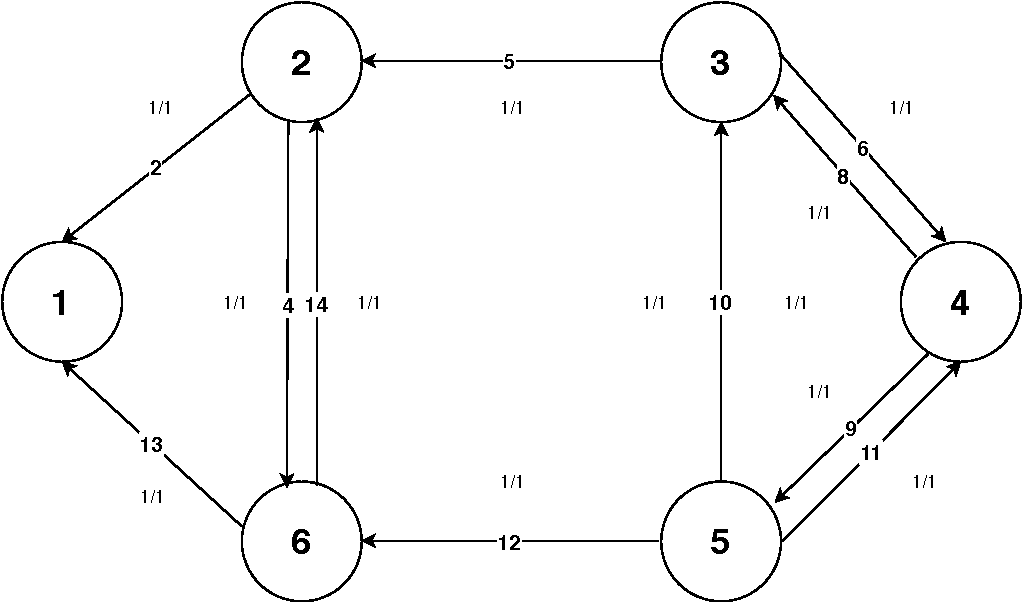
\includegraphics[width=12cm]{sdf/heuristic/transparent/figures/finalPhysicalTopology}
	\caption{Final physical topology graph.}
\end{figure}

\begin{table}[H]
	\centering
	\begin{tabular}{|c|c|c|c|c|c|}
		\hline
		\begin{tabular}[c]{@{}c@{}}opticalMultiplexing-\\ SystemIndex\end{tabular} & sourceNode & \begin{tabular}[c]{@{}c@{}}destination-\\ Node\end{tabular} & \begin{tabular}[c]{@{}c@{}}numberOf-\\ Wavelenghts\end{tabular} & \begin{tabular}[c]{@{}c@{}}wavelenghts\\ (nm)\end{tabular} & \begin{tabular}[c]{@{}c@{}}available-\\ Wavelenghts\end{tabular} \\ \hline
		0 & 1 & 2 & 2 & {[}1310 1550{]} & {[}0 0{]} \\ \hline
		1 & 1 & 6 & 2 & {[}1310 1550{]} & {[}0 0{]} \\ \hline
		2 & 2 & 1 & 2 & {[}1310 1550{]} & {[}1 1{]} \\ \hline
		3 & 2 & 3 & 2 & {[}1310 1550{]} & {[}0 0{]} \\ \hline
		4 & 2 & 6 & 2 & {[}1310 1550{]} & {[}1 1{]} \\ \hline
		5 & 3 & 2 & 2 & {[}1310 1550{]} & {[}1 1{]} \\ \hline
		6 & 3 & 4 & 2 & {[}1310 1550{]} & {[}0 1{]} \\ \hline
		7 & 3 & 5 & 2 & {[}1310 1550{]} & {[}0 0{]} \\ \hline
		8 & 4 & 3 & 2 & {[}1310 1550{]} & {[}1 1{]} \\ \hline
		9 & 4 & 5 & 2 & {[}1310 1550{]} & {[}0 1{]} \\ \hline
		10 & 5 & 3 & 2 & {[}1310 1550{]} & {[}1 1{]} \\ \hline
		11 & 5 & 4 & 2 & {[}1310 1550{]} & {[}1 1{]} \\ \hline
		12 & 5 & 6 & 2 & {[}1310 1550{]} & {[}1 1{]} \\ \hline
		13 & 6 & 1 & 2 & {[}1310 1550{]} & {[}1 1{]} \\ \hline
		14 & 6 & 2 & 2 & {[}1310 1550{]} & {[}1 1{]} \\ \hline
		15 & 6 & 5 & 2 & {[}1310 1550{]} & {[}0 0{]} \\ \hline
	\end{tabular}
	\caption{Final opticalMultiplexingSystems variable values.}
\end{table}

\clearpage
\section{Heuristics vs ILP}
\subsection{Low traffic scenario}

The traffic matrices below are represented by ODU0, ODU1, ODU2, ODU3 and ODU4 where each one has a certain bit rate. The ODU0 corresponds to 1.25 Gbits/s, the ODU1 corresponds to 2.5 Gbits/s, the ODU2 corresponds to 10 Gbits/s, the ODU3 corresponds to 40 Gbits/s and finally the ODU4 corresponds to 100 Gbits/s.\\ \\
%As we can see below, these arrays are bi-directional because they are symmetric arrays and as such, the traffic sent in a certain direction must be the same traffic sent in that opposite direction.
Considering 100 optical channels per opticalMultiplexingSystem, each with a capacity of 100 Gbps (80 ODU0s), and the following set of demands.\\ \\

\[
ODU0=
\begin{bmatrix}
0 & 5 & 1 & 3 & 1 & 3 \\
5 & 0 & 0 & 1 & 5 & 0 \\
1 & 0 & 0 & 1 & 4 & 1 \\
3 & 1 & 1 & 0 & 1 & 1 \\
1 & 5 & 4 & 1 & 0 & 3 \\
3 & 0 & 1 & 1 & 3 & 0
\end{bmatrix}
\qquad ODU1=
\begin{bmatrix}
0 & 2 & 4 & 2 & 0 & 5 \\
2 & 0 & 0 & 3 & 1 & 1 \\
4 & 0 & 0 & 1 & 1 & 0 \\
2 & 3 & 1 & 0 & 1 & 3 \\
0 & 1 & 1 & 1 & 0 & 1 \\
5 & 1 & 0 & 3 & 1 & 0
\end{bmatrix}
\]
\[
ODU2=
\begin{bmatrix}
0 & 1 & 1 & 1 & 0 & 0 \\
1 & 0 & 0 & 0 & 1 & 0 \\
1 & 0 & 0 & 1 & 1 & 0 \\
1 & 0 & 1 & 0 & 1 & 0 \\
0 & 1 & 1 & 1 & 0 & 1 \\
0 & 0 & 0 & 0 & 1 & 0
\end{bmatrix}
\qquad ODU3=
\begin{bmatrix}
0 & 0 & 0 & 0 & 0 & 0 \\
0 & 0 & 1 & 0 & 0 & 1 \\
0 & 1 & 0 & 0 & 1 & 0 \\
0 & 0 & 0 & 0 & 0 & 0 \\
0 & 0 & 1 & 0 & 0 & 0 \\
0 & 1 & 0 & 0 & 0 & 0
\end{bmatrix}
\]
\[
ODU4=
\begin{bmatrix}
0 & 0 & 0 & 0 & 0 & 0 \\
0 & 0 & 0 & 0 & 0 & 1 \\
0 & 0 & 0 & 0 & 0 & 0 \\
0 & 0 & 0 & 0 & 0 & 0 \\
0 & 0 & 0 & 0 & 0 & 1 \\
0 & 1 & 0 & 0 & 1 & 0
\end{bmatrix}
\]

\vspace{17pt}
Through these ODU's we can calculate the total network traffic for this specific scenario:\\

$T_1^0$ = 60x1.25 = 75 Gbits/s \qquad
$T_1^1$ = 50x2.5 = 125 Gbits/s \qquad
$T_1^2$ = 16x10 = 160 Gbits/s \\

$T_1^3$ = 6x40 = 240 Gbits/s \quad
$T_1^4$ = 4x100 = 400 Gbits/s \\

$T_{1}$ = 75 + 125 + 160 + 240 + 400 = 1000 Gbits/s \qquad \\
%$T$ = 1660/2 = \textbf{580 Gbits/s}\\

Where the variable $T_1^x$ represents the unidirectional traffic of the ODUx, for example, $T_1^0$ represents the unidirectional traffic of the ODU0 and $T_1^1$ represents the unidirectional traffic of the ODU1. The variable $T_{1}$ represents the total of unidirectional traffic that is injected into the network.\\
\begin{figure}[H]
	\centering
	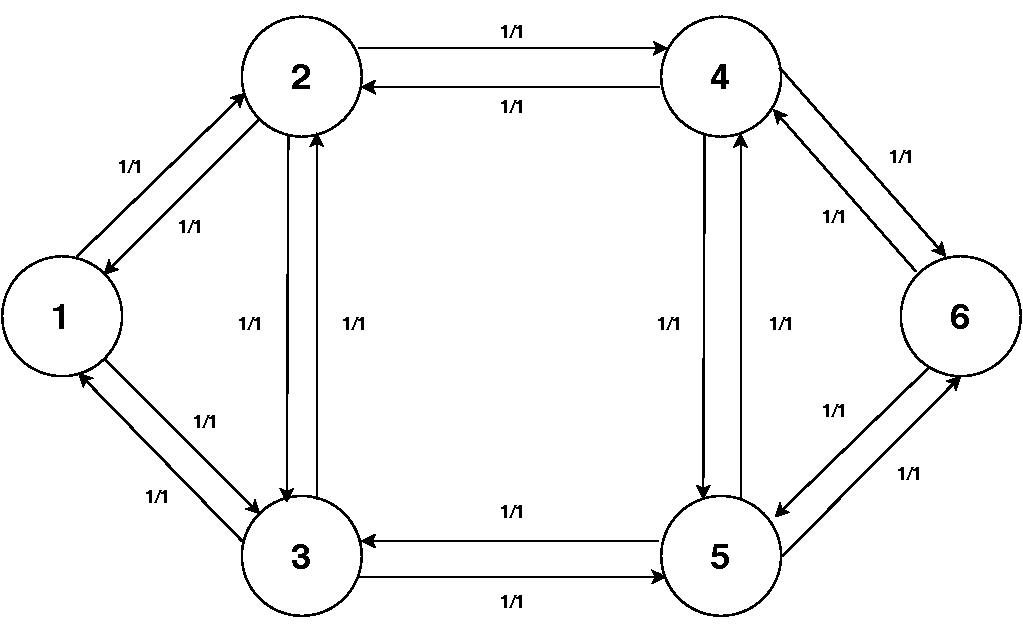
\includegraphics[width=15cm]{sdf/heuristic/transparent/figures/physicalTopology_low_traffic}
	\caption{Transparent without survivability in low scenario: physical topology after dimensioning.}
	\label{physical_topology_low_traffic}
\end{figure}
\begin{figure}[H]
	\centering
	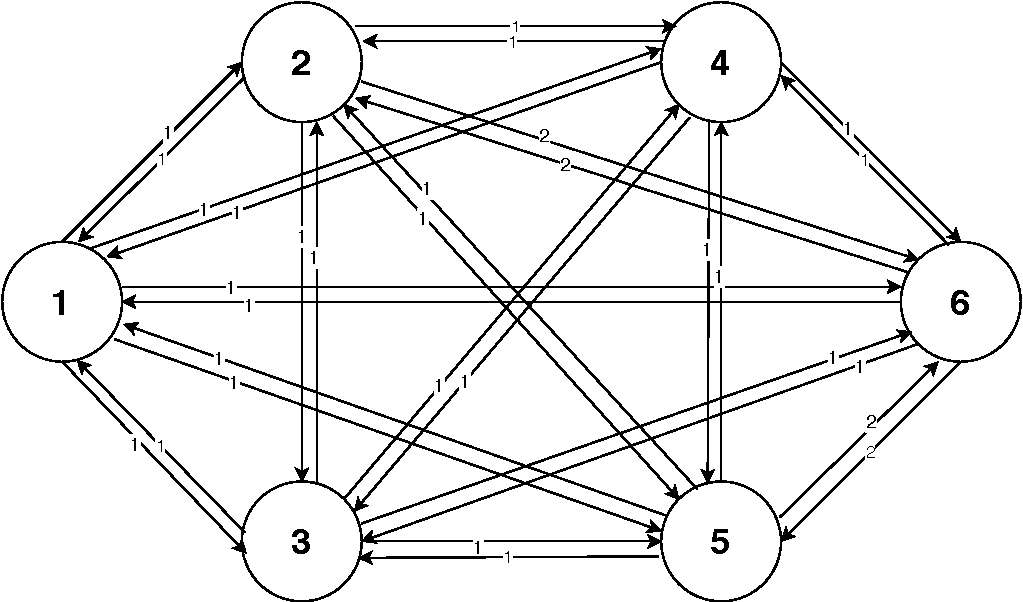
\includegraphics[width=15cm]{sdf/heuristic/transparent/figures/logicalTopology_low_traffic}
	\caption{Transparent without survivability in low scenario: opticall topology after dimensioning.}
\end{figure}

\begin{table}[H]
	\centering
	\begin{tabular}{|c|c|c|}
		\hline
		\multicolumn{3}{|c|}{\textbf{Information regarding links}} \\ \hline
		Unidirectional link & Optical channels & Amplifiers \\ \hline
		Node 1 -\textgreater 2 & 3 & 4 \\ \hline
		Node 1 -\textgreater 3 & 2 & 6 \\ \hline
		Node 2 -\textgreater 1 & 3 & 4 \\ \hline
		Node 2 -\textgreater 3 & 3 & 0 \\ \hline
		Node 2 -\textgreater 4 & 6 & 6 \\ \hline
		Node 3 -\textgreater 1 & 2 & 6 \\ \hline
		Node 3 -\textgreater 2 & 3 & 0 \\ \hline
		Node 3 -\textgreater 5 & 4 & 8 \\ \hline
		Node 4 -\textgreater 2 & 6 & 6 \\ \hline
		Node 4 -\textgreater 5 & 1 & 1 \\ \hline
		Node 4 -\textgreater 6 & 4 & 7 \\ \hline
		Node 5 -\textgreater 4 & 1 & 8 \\ \hline
		Node 5 -\textgreater 6 & 3 & 1 \\ \hline
		Node 5 -\textgreater 3 & 4 & 3 \\ \hline
		Node 6 -\textgreater 4 & 4 & 7 \\ \hline
		Node 6 -\textgreater 5 & 3 & 3 \\ \hline
	\end{tabular}
	\caption{Table with information regarding links for transparent mode without survivability in low
		scenario.}
\end{table}

\begin{table}[H]
	\centering
	\begin{tabular}{|c|c|c|c|c|c|}
		\hline
		\multicolumn{6}{|c|}{\textbf{Information regarding nodes}} \\ \hline
		\multicolumn{2}{|c|}{} & \multicolumn{2}{c|}{Electrical part} & \multicolumn{2}{c|}{Optical part} \\ \hline
		Node & Nodal degree & Tributary ports & LR transponders & Add ports & Line ports \\ \hline
		1 & 2 & 29 & 5 & 5 & 5 \\ \hline
		2 & 3 & 23 & 6 & 6 & 12 \\ \hline
		3 & 3 & 18 & 5 & 5 & 9 \\ \hline
		4 & 3 & 20 & 5 & 5 & 11 \\ \hline
		5 & 3 & 24 & 6 & 6 & 8 \\ \hline
		6 & 2 & 22 & 7 & 7 & 7 \\ \hline
	\end{tabular}
	\caption{Table with information regarding nodes for transparent mode without survivability in low
	scenario.}
\end{table}
\begin{table}[H]
	\centering
	\begin{tabular}{|c|c|c|c|c|c|c|c|}
		\hline
		\multicolumn{8}{|c|}{\textbf{Routing}} \\ \hline
		\textbf{Source node} & \textbf{Destination node} & \textbf{Links} & \textbf{ODU0} & \textbf{ODU1} & \textbf{ODU2} & \textbf{ODU3} & \textbf{ODU4} \\ \hline
		1 & 2 & \{(1,2)\} & 5 & 2 & 1 & 0 & 0 \\ \hline
		1 & 3 & \{(1,3)\} & 1 & 4 & 1 & 0 & 0 \\ \hline
		1 & 4 & \{(1,2),(2,4)\} & 3 & 2 & 1 & 0 & 0 \\ \hline
		1 & 5 & \{(1,3),(3,5)\} & 1 & 0 & 0 & 0 & 0 \\ \hline
		1 & 6 & \{(1,2),(2,4),(4,6)\} & 3 & 5 & 0 & 0 & 0 \\ \hline
		2 & 1 & \{(2,1)\} & 5 & 2 & 1 & 0 & 0 \\ \hline
		2 & 3 & \{(2,3)\} & 0 & 0 & 0 & 1 & 0 \\ \hline
		2 & 4 & \{(2,4)\} & 1 & 3 & 0 & 0 & 0 \\ \hline
		2 & 5 & \{(2,3),(3,5)\} & 5 & 1 & 1 & 0 & 0 \\ \hline
		2 & 6 & \{(2,4),(2,6)\} & 0 & 1 & 0 & 1 & 1 \\ \hline
		3 & 1 & \{(1,3)\} & 1 & 4 & 1 & 0 & 0 \\ \hline
		3 & 2 & \{(3,2)\} & 0 & 0 & 0 & 1 & 0 \\ \hline
		3 & 4 & \{(3,2),(2,4)\} & 1 & 1 & 1 & 0 & 0 \\ \hline
		3 & 5 & \{(3,5)\} & 4 & 1 & 1 & 1 & 0 \\ \hline
		3 & 6 & \{(3,5),(5,6)\} & 1 & 0 & 0 & 0 & 0 \\ \hline
		4 & 1 & \{(4,2),(2,1)\} & 3 & 2 & 1 & 0 & 0 \\ \hline
		4 & 2 & \{(4,2)\} & 1 & 3 & 0 & 0 & 0 \\ \hline
		4 & 3 & \{(4,2),(2,3)\} & 1 & 1 & 1 & 0 & 0 \\ \hline
		4 & 5 & \{(4,5)\} & 1 & 1 & 1 & 0 & 0 \\ \hline
		4 & 6 & \{(4,6)\} & 1 & 3 & 0 & 0 & 0 \\ \hline
		5 & 1 & \{(5,3)(3,1)\} & 1 & 0 & 0 & 0 & 0 \\ \hline
		5 & 2 & \{(5,3),(3,2)\} & 5 & 1 & 1 & 0 & 0 \\ \hline
		5 & 3 & \{(5,3)\} & 4 & 1 & 1 & 1 & 0 \\ \hline
		5 & 4 & \{(5,4)\} & 1 & 1 & 1 & 0 & 0 \\ \hline
		5 & 6 & \{(5,6)\} & 3 & 1 & 1 & 0 & 1 \\ \hline
		6 & 1 & \{(6,4),(4,2),(2,1)\} & 3 & 5 & 0 & 0 & 0 \\ \hline
		6 & 2 & \{(6,4),(4,2)\} & 0 & 1 & 0 & 1 & 1 \\ \hline
		6 & 3 & \{(6,5),(5,3)\} & 1 & 0 & 0 & 0 & 0 \\ \hline
		6 & 4 & \{(6,4)\} & 1 & 3 & 0 & 0 & 0 \\ \hline
		6 & 5 & \{(6,5)\} & 3 & 1 & 1 & 0 & 1 \\ \hline
	\end{tabular}
	\caption{Transparent without survivability in low scenario: description of routing.}
\end{table}
\begin{table}[H]
	\begin{tabular}{|c|c|c|c|c|c|c|}
		\hline
		\multicolumn{7}{|c|}{\textbf{Network CAPEX}} \\ \hline
		\multicolumn{3}{|c|}{} & \textbf{Quantity} & \textbf{Unit price} & \textbf{Cost} & \textbf{Total} \\ \hline
		\multirow{3}{*}{Link cost} & \multicolumn{2}{c|}{OLTs} & 16 & 15 000 \euro & 240 000 \euro & \multirow{3}{*}{26 520 000 \euro} \\ \cline{2-6}
		& \multicolumn{2}{c|}{100 Gbit/s Transceivers} & 52 & 5 000 \euro /Gbit/s & 26 000 000 \euro &  \\ \cline{2-6}
		& \multicolumn{2}{c|}{Amplifiers} & 70 & 10 000 \euro & 280 000 \euro &  \\ \hline
		\multirow{10}{*}{Node Cost} & \multirow{7}{*}{Electrical part} & EXCs & 6 & 10 000 \euro & 60 000 \euro & \multirow{10}{*}{3 797 590 \euro} \\ \cline{3-6}
		&  & ODU0 ports & 60 & 10 \euro/ port & 600 \euro &  \\ \cline{3-6}
		&  & ODU1 ports & 50 & 15 \euro/ port & 750 \euro &  \\ \cline{3-6}
		&  & ODU2 ports & 16 & 30 \euro/ port & 480 \euro &  \\ \cline{3-6}
		&  & ODU3 ports & 6 & 60 \euro/ port & 360 \euro &  \\ \cline{3-6}
		&  & ODU4 ports & 4 & 100 \euro/ port & 400 \euro &  \\ \cline{3-6}
		&  & Transponders & 34 & 100 000 \euro/ port & 3 400 000 \euro &  \\ \cline{2-6}
		& \multirow{3}{*}{Optical part} & OXCs & 6 & 20 000 \euro & 120 000 \euro &  \\ \cline{3-6}
		&  & Add ports & 34 & 2500 \euro/port & 85 000 \euro &  \\ \cline{3-6}
		&  & Line ports & 52 & 2500 \euro/ port & 130 000 \euro &  \\ \hline
		\multicolumn{6}{|c|}{Total Network Cost} & 30 317 590 \euro \\ \hline
	\end{tabular}
	\caption{Transparent without survivability in low scenario: detailed description of CAPEX for this
		scenario.}
\end{table}

\subsection{Medium traffic scenario}

\[
ODU0=
\begin{bmatrix}
	0 & 50 & 10 & 30 & 10 & 30 \\
	50 & 0 & 0 & 10 & 50 & 0 \\
	10 & 0 & 0 & 10 & 40 & 10 \\
	30 & 10 & 10 & 0 & 10 & 10 \\
	10 & 50 & 40 & 10 & 0 & 30 \\
	30 & 0 & 10 & 10 & 30 & 0
\end{bmatrix}
\qquad ODU1=
\begin{bmatrix}
	0 & 20 & 40 & 20 & 0 & 50 \\
	20 & 0 & 0 & 30 & 10 & 10 \\
	40 & 0 & 0 & 10 & 10 & 0 \\
	20 & 30 & 10 & 0 & 10 & 30 \\
	0 & 10 & 10 & 10 & 0 & 10 \\
	50 & 10 & 0 & 30 & 10 & 0
\end{bmatrix}
\]
\[
ODU2=
\begin{bmatrix}
0 & 10 & 10 & 10 & 0 & 0 \\
10 & 0 & 0 & 0 & 10 & 0 \\
10 & 0 & 0 & 10 & 10 & 0 \\
10 & 0 & 10 & 0 & 10 & 0 \\
0 & 10 & 10 & 10 & 0 & 10 \\
0 & 0 & 0 & 0 & 10 & 0
\end{bmatrix}
\qquad ODU3=
\begin{bmatrix}
0 & 0 & 0 & 0 & 0 & 0 \\
0 & 0 & 10 & 0 & 0 & 10 \\
0 & 10 & 0 & 0 & 10 & 0 \\
0 & 0 & 0 & 0 & 0 & 0 \\
0 & 0 & 10 & 0 & 0 & 0 \\
0 & 10 & 0 & 0 & 0 & 0
\end{bmatrix}
\]
\[
ODU4=
\begin{bmatrix}
0 & 0 & 0 & 0 & 0 & 0 \\
0 & 0 & 0 & 0 & 0 & 10 \\
0 & 0 & 0 & 0 & 0 & 0 \\
0 & 0 & 0 & 0 & 0 & 0 \\
0 & 0 & 0 & 0 & 0 & 10 \\
0 & 10 & 0 & 0 & 10 & 0
\end{bmatrix}
\]

\vspace{17pt}
Through these ODU's we can calculate the total network traffic for this specific scenario:\\

$T_1^0$ = 600x1.25 = 750 Gbits/s \qquad
$T_1^1$ = 500x2.5 = 1250 Gbits/s \qquad
$T_1^2$ = 160x10 = 1600 Gbits/s \\

$T_1^3$ = 60x40 = 2400 Gbits/s \quad
$T_1^4$ = 40x100 = 4000 Gbits/s \\

$T_{1}$ = 750 + 1250 + 1600 + 2400 + 4000 = 10000 Gbits/s \qquad \\
%$T$ = 1660/2 = \textbf{580 Gbits/s}\\

\begin{figure}[H]
	\centering
	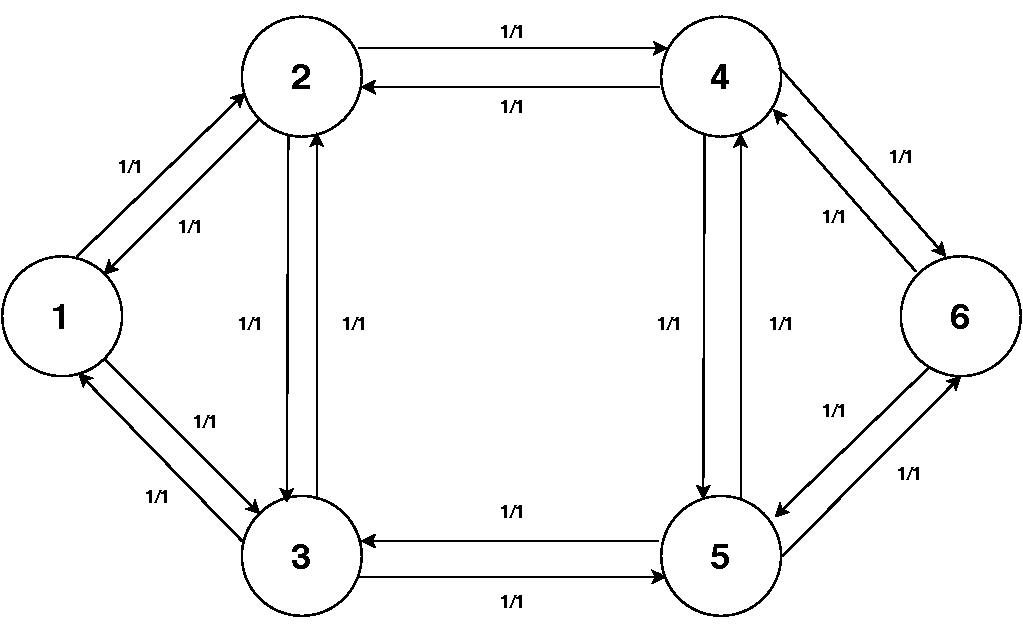
\includegraphics[width=15cm]{sdf/heuristic/transparent/figures/physicalTopology_low_traffic}
	\caption{Transparent without survivability in medium scenario: physical topology after dimensioning.}
	\label{physical_topology_medium_traffic}
\end{figure}

\begin{table}[H]
	\centering
	\begin{tabular}{|c|c|c|}
		\hline
		\multicolumn{3}{|c|}{\textbf{Information regarding links}} \\ \hline
		Unidirectional link & Optical channels & Amplifiers \\ \hline
		Node 1 -\textgreater 2 & 7 & 4 \\ \hline
		Node 1 -\textgreater 3 & 4 & 6 \\ \hline
		Node 2 -\textgreater 1 & 7 & 4 \\ \hline
		Node 2 -\textgreater 3 & 9 & 0 \\ \hline
		Node 2 -\textgreater 4 & 22 & 6 \\ \hline
		Node 3 -\textgreater 1 & 4 & 6 \\ \hline
		Node 3 -\textgreater 2 & 9 & 0 \\ \hline
		Node 3 -\textgreater 5 & 10 & 8 \\ \hline
		Node 4 -\textgreater 2 & 22 & 6 \\ \hline
		Node 4 -\textgreater 5 & 2 & 1 \\ \hline
		Node 4 -\textgreater 6 & 18 & 7 \\ \hline
		Node 5 -\textgreater 4 & 2 & 1 \\ \hline
		Node 5 -\textgreater 6 & 13 & 3 \\ \hline
		Node 5 -\textgreater 3 & 10 & 8 \\ \hline
		Node 6 -\textgreater 4 & 18 & 7 \\ \hline
		Node 6 -\textgreater 5 & 13 & 3 \\ \hline
	\end{tabular}
	\caption{Table with information regarding links for transparent mode without survivability in medium traffic scenario.}
\end{table}

\begin{table}[H]
	\centering
	\begin{tabular}{|c|c|c|c|c|c|}
		\hline
		\multicolumn{6}{|c|}{\textbf{Information regarding nodes}} \\ \hline
		\multicolumn{2}{|c|}{} & \multicolumn{2}{c|}{Electrical part} & \multicolumn{2}{c|}{Optical part} \\ \hline
		Node & Nodal degree & Tributary ports & LR transponders & Add ports & Line ports \\ \hline
		1 & 2 & 290 & 11 & 11 & 11 \\ \hline
		2 & 3 & 230 & 26 & 26 & 38 \\ \hline
		3 & 3 & 180 & 17 & 17 & 23 \\ \hline
		4 & 3 & 200 & 8 & 8 & 42 \\ \hline
		5 & 3 & 240 & 23 & 23 & 25 \\ \hline
		6 & 2 & 220 & 31 & 31 & 31 \\ \hline
	\end{tabular}
	\caption{Table with information regarding nodes for transparent mode without survivability in medium traffic scenario.}
\end{table}

\begin{table}[H]
	\begin{tabular}{|c|c|c|c|c|c|c|}
		\hline
		\multicolumn{7}{|c|}{\textbf{Network CAPEX}} \\ \hline
		\multicolumn{3}{|c|}{} & \textbf{Quantity} & \textbf{Unit price} & \textbf{Cost} & \textbf{Total} \\ \hline
		\multirow{3}{*}{Link cost} & \multicolumn{2}{c|}{OLTs} & 16 & 15 000 \euro & 240 000 \euro & \multirow{3}{*}{85 520 000 \euro} \\ \cline{2-6}
		& \multicolumn{2}{c|}{100 Gbit/s Transceivers} & 170 & 5 000 \euro/Gbit/s & 85 000 000 \euro &  \\ \cline{2-6}
		& \multicolumn{2}{c|}{Amplifiers} & 70 & 10 000 \euro & 280 000 \euro &  \\ \hline
		\multirow{10}{*}{Node Cost} & \multirow{7}{*}{Electrical part} & EXCs & 6 & 10 000 \euro & 60 000 \euro & \multirow{10}{*}{12 520 900 \euro} \\ \cline{3-6}
		&  & ODU0 ports & 600 & 10 \euro/ port & 6000 \euro &  \\ \cline{3-6}
		&  & ODU1 ports & 500 & 15 \euro/ port & 7500 \euro &  \\ \cline{3-6}
		&  & ODU2 ports & 160 & 30 \euro/ port & 4800 \euro &  \\ \cline{3-6}
		&  & ODU3 ports & 60 & 60 \euro/ port & 3600 \euro &  \\ \cline{3-6}
		&  & ODU4 ports & 40 & 100 \euro/ port & 4000 \euro &  \\ \cline{3-6}
		&  & Transponders & 116 & 100 000 \euro/ port & 11 600 000 \euro &  \\ \cline{2-6}
		& \multirow{3}{*}{Optical part} & OXCs & 6 & 20 000 \euro & 120 000 \euro &  \\ \cline{3-6}
		&  & Add ports & 116 & 2500 \euro/port & 290 000 \euro &  \\ \cline{3-6}
		&  & Line ports & 170 & 2500 \euro/ port & 425 000 \euro &  \\ \hline
		\multicolumn{6}{|c|}{Total Network Cost} & 98 040 900 \euro \\ \hline
	\end{tabular}
	\caption{Transparent without survivability in medium traffic scenario: detailed description of CAPEX for this scenario.}
\end{table}

\subsection{High traffic scenario}

\[
ODU0=
\begin{bmatrix}
0 & 100 & 20 & 60 & 20 & 60 \\
100 & 0 & 0 & 20 & 100 & 0 \\
20 & 0 & 0 & 20 & 80 & 20 \\
60 & 20 & 20 & 0 & 20 & 20 \\
20 & 100 & 80 & 20 & 0 & 60 \\
60 & 0 & 20 & 20 & 60 & 0
\end{bmatrix}
\qquad ODU1=
\begin{bmatrix}
0 & 40 & 80 & 40 & 0 & 100 \\
40 & 0 & 0 & 60 & 20 & 20 \\
80 & 0 & 0 & 20 & 20 & 0 \\
40 & 60 & 20 & 0 & 20 & 60 \\
0 & 20 & 20 & 20 & 0 & 20 \\
100 & 20 & 0 & 60 & 20 & 0
\end{bmatrix}
\]
\[
ODU2=
\begin{bmatrix}
0 & 20 & 20 & 20 & 0 & 0 \\
20 & 0 & 0 & 0 & 20 & 0 \\
20 & 0 & 0 & 20 & 20 & 0 \\
20 & 0 & 20 & 0 & 20 & 0 \\
0 & 20 & 20 & 20 & 0 & 20 \\
0 & 0 & 0 & 0 & 20 & 0
\end{bmatrix}
\qquad ODU3=
\begin{bmatrix}
0 & 0 & 0 & 0 & 0 & 0 \\
0 & 0 & 20 & 0 & 0 & 20 \\
0 & 20 & 0 & 0 & 20 & 0 \\
0 & 0 & 0 & 0 & 0 & 0 \\
0 & 0 & 20 & 0 & 0 & 0 \\
0 & 20 & 0 & 0 & 0 & 0
\end{bmatrix}
\]
\[
ODU4=
\begin{bmatrix}
0 & 0 & 0 & 0 & 0 & 0 \\
0 & 0 & 0 & 0 & 0 & 20 \\
0 & 0 & 0 & 0 & 0 & 0 \\
0 & 0 & 0 & 0 & 0 & 0 \\
0 & 0 & 0 & 0 & 0 & 20 \\
0 & 20 & 0 & 0 & 20 & 0
\end{bmatrix}
\]

\vspace{17pt}
Through these ODU's we can calculate the total network traffic for this specific scenario:\\

$T_1^0$ = 600x1.25 = 750 Gbits/s \qquad
$T_1^1$ = 500x2.5 = 1250 Gbits/s \qquad
$T_1^2$ = 160x10 = 1600 Gbits/s \\

$T_1^3$ = 60x40 = 2400 Gbits/s \quad
$T_1^4$ = 40x100 = 4000 Gbits/s \\

$T_{1}$ = 750 + 1250 + 1600 + 2400 + 4000 = 10000 Gbits/s \qquad \\
%$T$ = 1660/2 = \textbf{580 Gbits/s}\\

\begin{figure}[H]
	\centering
	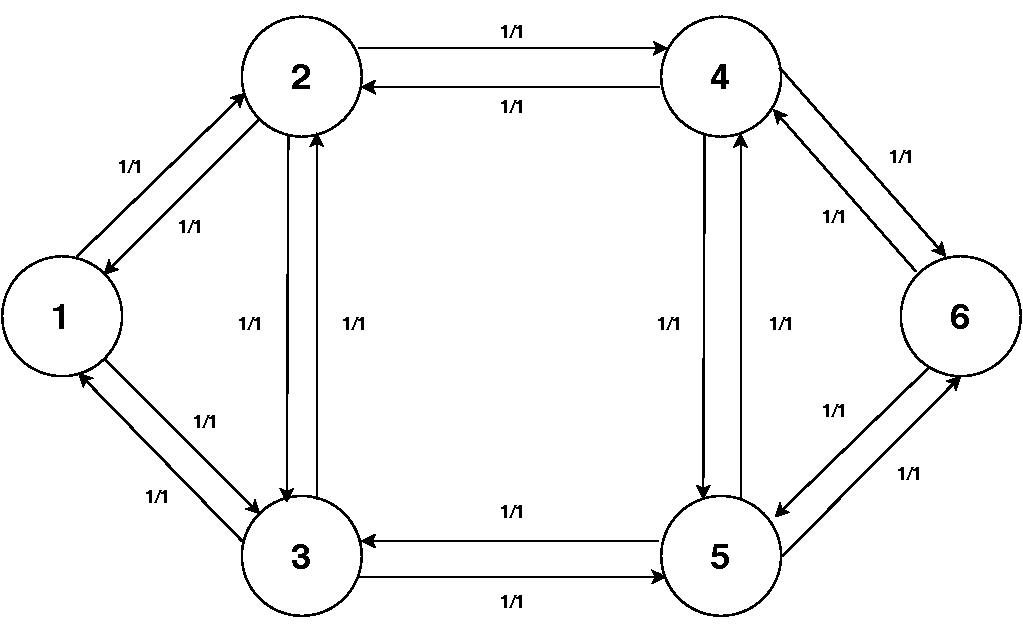
\includegraphics[width=15cm]{sdf/heuristic/transparent/figures/physicalTopology_low_traffic}
	\caption{Transparent without survivability in high scenario: physical topology after dimensioning.}
	\label{physical_topology_medium_traffic}
\end{figure}

\begin{table}[H]
	\centering
	\begin{tabular}{|c|c|c|}
		\hline
		\multicolumn{3}{|c|}{\textbf{Information regarding links}} \\ \hline
		Unidirectional link & Optical channels & Amplifiers \\ \hline
		Node 1 -\textgreater 2 & 13 & 4 \\ \hline
		Node 1 -\textgreater 3 & 6 & 6 \\ \hline
		Node 2 -\textgreater 1 & 13 & 4 \\ \hline
		Node 2 -\textgreater 3 & 17 & 0 \\ \hline
		Node 2 -\textgreater 4 & 43 & 6 \\ \hline
		Node 3 -\textgreater 1 & 6 & 6 \\ \hline
		Node 3 -\textgreater 2 & 17 & 0 \\ \hline
		Node 3 -\textgreater 5 & 18 & 8 \\ \hline
		Node 4 -\textgreater 2 & 43 & 6 \\ \hline
		Node 4 -\textgreater 5 & 3 & 1 \\ \hline
		Node 4 -\textgreater 6 & 36 & 7 \\ \hline
		Node 5 -\textgreater 3 & 18 & 8 \\ \hline
		Node 5 -\textgreater 4 & 3 & 1 \\ \hline
		Node 5 -\textgreater 6 & 25 & 3 \\ \hline
		Node 6 -\textgreater 4 & 36 & 7 \\ \hline
		Node 6 -\textgreater 5 & 25 & 3 \\ \hline
	\end{tabular}
	\caption{Table with information regarding links for transparent mode without survivability in high traffic scenario.}
\end{table}


\begin{table}[H]
	\centering
	\begin{tabular}{|c|c|c|c|c|c|}
		\hline
		\multicolumn{6}{|c|}{\textbf{Information regarding nodes}} \\ \hline
		\multicolumn{2}{|c|}{} & \multicolumn{2}{c|}{Electrical part} & \multicolumn{2}{c|}{Optical part} \\ \hline
		Node & Nodal degree & Tributary ports & LR transponders & Add ports & Line ports \\ \hline
		1 & 2 & 580 & 19 & 19 & 19 \\ \hline
		2 & 3 & 460 & 51 & 51 & 73 \\ \hline
		3 & 3 & 360 & 31 & 31 & 41 \\ \hline
		4 & 3 & 400 & 14 & 14 & 82 \\ \hline
		5 & 3 & 480 & 44 & 44 & 46 \\ \hline
		6 & 2 & 440 & 61 & 61 & 61 \\ \hline
	\end{tabular}
	\caption{Table with information regarding nodes for transparent mode without survivability in high traffic scenario.}
\end{table}

\begin{table}[H]
	\begin{tabular}{|c|c|c|c|c|c|c|}
		\hline
		\multicolumn{7}{|c|}{\textbf{Network CAPEX}} \\ \hline
		\multicolumn{3}{|c|}{} & \textbf{Quantity} & \textbf{Unit price} & \textbf{Cost} & \textbf{Total} \\ \hline
		\multirow{3}{*}{Link cost} & \multicolumn{2}{c|}{OLTs} & 16 & 15 000 \euro & 240 000 \euro & \multirow{3}{*}{161 520 000 \euro} \\ \cline{2-6}
		& \multicolumn{2}{c|}{100 Gbit/s Transceivers} & 322 & 5 000 \euro/Gbit/s & 110 000 000 \euro &  \\ \cline{2-6}
		& \multicolumn{2}{c|}{Amplifiers} & 70 & 10 000 \euro & 280 000 \euro &  \\ \hline
		\multirow{10}{*}{Node Cost} & \multirow{7}{*}{Electrical part} & EXCs & 6 & 10 000 \euro & 60 000 \euro & \multirow{10}{*}{23 586 800 \euro} \\ \cline{3-6}
		&  & ODU0 ports & 1200 & 10 \euro/ port & 12 000 \euro &  \\ \cline{3-6}
		&  & ODU1 ports & 1000 & 15 \euro/ port & 15 000 \euro &  \\ \cline{3-6}
		&  & ODU2 ports & 320 & 30 \euro/ port & 9600 \euro &  \\ \cline{3-6}
		&  & ODU3 ports & 120 & 60 \euro/ port & 7200 \euro &  \\ \cline{3-6}
		&  & ODU4 ports & 80 & 100 \euro/ port & 8000 \euro &  \\ \cline{3-6}
		&  & Transponders & 220 & 100 000 \euro/ port & 22 000 000 \euro &  \\ \cline{2-6}
		& \multirow{3}{*}{Optical part} & OXCs & 6 & 20 000 \euro & 120 000 \euro &  \\ \cline{3-6}
		&  & Add ports & 220 & 2500 \euro/port & 550 000 \euro &  \\ \cline{3-6}
		&  & Line ports & 322 & 2500 \euro/ port & 805 000 \euro &  \\ \hline
		\multicolumn{6}{|c|}{Total Network Cost} & 185 106 800 \euro \\ \hline
	\end{tabular}
	\caption{Transparent without survivability in high traffic scenario: detailed description of CAPEX for this scenario.}
\end{table}

\begin{table}[H]
	\begin{tabular}{|c|l|l|l|l|}
		\hline
		\multicolumn{2}{|c|}{} & \multicolumn{1}{c|}{\textbf{ILP}} & \multicolumn{1}{c|}{\textbf{Other Heuristics}} & \multicolumn{1}{c|}{\textbf{My Heuristics}} \\ \hline
		\textbf{Low traffic} & \begin{tabular}[c]{@{}l@{}}Link cost\\ Node Cost\\ \\ CAPEX\end{tabular} & \begin{tabular}[c]{@{}l@{}}26 520 000 \euro\\ 3 797 590 \euro \\ \\ 30 317 590 \euro\end{tabular} & \begin{tabular}[c]{@{}l@{}}26 520 000 \euro\\ 3 797 590 \euro\\ \\ 30 317 590 \euro\end{tabular} & \begin{tabular}[c]{@{}l@{}}26 520 000 \euro \\ 3 797 590 \euro\\ \\ 30 317 590 \euro\end{tabular} \\ \hline
		\textbf{Medium traffic} & \begin{tabular}[c]{@{}l@{}}Link cost\\ Node Cost\\ \\ CAPEX\end{tabular} & \begin{tabular}[c]{@{}l@{}}84 520 000 \euro\\ 12 310 900 \euro\\ \\ 96 830 900 \euro\end{tabular} & \begin{tabular}[c]{@{}l@{}}84 520 000 \euro\\ 15 180 900 \euro\\ \\ 99 700 900 \euro\end{tabular} & \begin{tabular}[c]{@{}l@{}}85 520 000 \euro\\ 12 520 900 \euro\\ \\ 98 040 900 \euro\end{tabular} \\ \hline
		\textbf{High traffic} & \begin{tabular}[c]{@{}l@{}}Link cost\\ Node Cost\\ \\ CAPEX\end{tabular} & \begin{tabular}[c]{@{}l@{}}157 520 000 \euro\\ 22 951 800 \euro\\ \\ 180 471 800 \euro\end{tabular} & \begin{tabular}[c]{@{}l@{}}157 520 000 \euro\\ 28 486 800 \euro\\ \\ 186 006 800 \euro\end{tabular} & \begin{tabular}[c]{@{}l@{}}161 520 000 \euro\\ 23 586 800 \euro\\ \\ 185 106 800 \euro\end{tabular} \\ \hline
	\end{tabular}
	\caption{Transparent without survivability: Table with different value of CAPEX for all scenarios}
\end{table}